\documentclass[12pt]{article}
\usepackage{float}
\usepackage[margin=1in,nohead]{geometry}
\usepackage{xltabular,booktabs,tabularx}
\usepackage[labelfont=bf, font=footnotesize, width=1\textwidth]{caption}
\usepackage{ifxetex,ifluatex}
\usepackage{mathptmx,amsbsy,latexsym,amsfonts,amsthm,amsmath,amssymb,mathtools}
\usepackage{setspace,array,accents,dcolumn,adjustbox}
\usepackage{graphicx}
\usepackage[mathscr]{eucal}
\usepackage{xcolor,colortbl,soul}
\usepackage{comment}
\usepackage{natbib}
\usepackage{xurl}
\usepackage{setspace}
\usepackage{titlesec}
\usepackage{siunitx}
\usepackage{comment}

\ifnum 0\ifxetex 1\fi\ifluatex 1\fi=0 % if pdftex
  \usepackage[T1]{fontenc}
  \usepackage[utf8]{inputenc}
  \usepackage{textcomp} % provide euro and other symbols
\else % if luatex or xetex
  \usepackage{unicode-math}
  \defaultfontfeatures{Scale=MatchLowercase}
  \defaultfontfeatures[\rmfamily]{Ligatures=TeX,Scale=1}
\fi

\sisetup{output-exponent-marker=\ensuremath{\mathrm{e}}}
\urlstyle{same}
\bibliographystyle{agms}
\titleformat*{\paragraph}{\itshape}
\titlespacing*{\paragraph}{0pt}{2ex}{.5em}
\newcolumntype{Y}{>{\centering\arraybackslash}X}
\def\naive{na\"{\i}ve }

\newcommand{\Section}[1]{\vspace{-8pt}\section{\hskip -1em.~~#1}\vspace{-3pt}}
\newcommand{\SubSection}[1]{\vspace{-3pt}\subsection{\hskip -1em.~~#1}\vspace{-3pt}}
\renewcommand{\theenumi}{\roman{enumi}}
\newcommand{\mc}{\multicolumn}

\DeclareMathOperator*{\argmax}{argmax}
\DeclareMathOperator*{\sgn}{sgn}
\DeclarePairedDelimiter\abs{\lvert}{\rvert}
\newcommand{\lowerbar}[1]{\underaccent{\bar}{#1}}

\renewcommand{\qed}{{\it Q.E.D.}}
\newcommand{\efficacy}{\phi}
\newcommand{\side}{s}
\newcommand{\general}{g}
\newcommand{\benefit}{B}
\newcommand{\ratio}{\rho^0\!}

\newcommand{\xuniv}{x^{u}}
\newcommand{\Xuniv}{X^{u}}
\newcommand{\xunivlbar}{\lowerbar{x}^{u}}

\newcommand{\xshort}{x^{s}}
\newcommand{\Xshort}{X^{s}}
\newcommand{\xshortbar}{\bar{x}^{\,s}}

\newcommand{\xunit}{x^{e}}
\newcommand{\xunitbar}{\bar{x}^{\,e}}

\newcommand{\xpoi}{x^{i}}
\newcommand{\xpeak}{x^{p}}

\newcommand{\xno}{x^{0}}
\newcommand{\Xno}{X^{0}}
\newcommand{\xnobar}{\bar{x}^{\,0}}
\newcommand{\xnolbar}{\lowerbar{x}^0}

\newcommand{\nno}{n^{0}}
\newcommand{\nnobar}{\bar{n}^{0}}
\newcommand{\vno}{v^{0}}
\newcommand{\vnobar}{\bar{v}^{0}}
\newcommand{\Qno}{Q^{0}}

\newcommand{\Qhat}{\hat{Q}}

\newcommand{\MB}{\text{\it MB}}
\newcommand{\Lagrangian}{\mathscr{L}}
\newcommand{\elasticity}[1]{\eta_{#1}}
\newcommand{\perunit}[1]{\alpha_{#1}}
\newcommand{\covid}{Covid-19}
\newcommand{\alldeaths}{\text{\it AD}}

\newcommand{\etilde}{\tilde{\epsilon}}
\newcommand{\xtilde}{\tilde{x}}
\newcommand{\Qtilde}{\tilde{Q}}
\newcommand{\vtilde}{\tilde{v}}

\newcommand{\benefitbound}{\bar{\benefit}}
\newcommand{\Rzero}{\mathcal{R}_0}

\newcommand{\Wiecek}{Wi\k{e}cek}
\newcommand{\pkg}[1]{\textit{#1}}

\newtheorem{lemma}{Lemma}
\newtheorem{proposition}{Proposition}
\newtheorem{corollary}{Corollary}

\def\topfraction{.9}
\def\floatpagefraction{.8}
\allowdisplaybreaks[1]
\setlength{\parindent}{20pt}

\begin{document}

\begin{spacing}{1.44}

%%%%%%%%%%%%%%%%%%%%%%%%%%%%%%%%%%%%%%%%%%%%%%%%%%%%%%%%%%%%%%%%%%%%%%%%%%%%%%%
\begin{titlepage}
\singlespace

\begin{center}
{\large \bf Optimal Dose Stretching Under Vaccine Supply Constraints}
\end{center}

\vspace{2ex}

{\flushleft
Michael Kremer\\
{\em Kenneth C. Griffin Department of Economics, University of Chicago\\ 
E-mail: kremermr@uchicago.edu}\\[2ex]
Christopher M. Snyder\\
{\em Department of Economics, Dartmouth College\\
E-mail: chris.snyder@dartmouth.edu}\\[2ex]
Witold \Wiecek\\
{\em Development Innovation Lab, University of Chicago\\
E-mail: witold.wiecek@gmail.com}}

\vspace{2ex}

\begin{center}
October 2026
\end{center}

\vspace{2ex}

\noindent {\bf Abstract:} The urgency to quell an epidemic by
vaccinating a large population as quickly as possible can lead to
shortages, which can be alleviated with fractional doses. We study
optimal fractional dosing in a tractable model capturing the essence
of more complex epidemiological studies. Under a concave dose-response
function, fractional dosing is always optimal if supplies are
insufficient to deliver full doses to the entire population, and
optimal dose strength is weakly increasing in vaccine supply. The same
is often true under an s-shaped dose-response function, although
exceptions can arise where a further tightening of extremely scarce
supplies leads to more concentrated doses. The analysis then shifts to
deriving quantitative results from a dynamic epidemiological model,
allowing mortality and disease transmission to vary by age, calibrated
to \covid\ parameters. The gains from fractional dosing can be
substantial, reducing mortality under full doses by
as much as 35\%.

\vfill

\noindent {\bf JEL Codes:} I18 (Health: Government Policy, Public
Health); O38 (Innovation: Government Policy); C63 (Simulation
Modeling)

\vfill

\noindent {\bf Keywords:} vaccine, pandemic, epidemiology, dose
response, supply

\vfill

\noindent {\bf Acknowledgments:} The authors are grateful to Rachel
Glennerster, Nora Szech, and seminar participants at Harvard, M.I.T.,
University of Chicago, the Dartmouth Health Economics and Policy Lab, and the NBER Entrepreneurship and Innovation
Policy and the Economy conference for insightful comments. Andreas
Petrou-Zeniou, Alexandre Simoes Gomes, and Leonardo Wang provided
excellent research assistance. Kremer and Snyder thank their
colleagues at the Market Shaping Accelerator for advice and
support. Funding from the Peter G. Peterson Foundation Pandemic
Response Policy Research Fund is gratefully acknowledged.

\end{titlepage}

%%%%%%%%%%%%%%%%%%%%%%%%%%%%%%%%%%%%%%%%%%%%%%%%%%%%%%%%%%%%%%%%%%%%%%%%%%%%%%%

\Section{Introduction}
\label{s:Introduction}

In an epidemic, infections and consequent demand for vaccines can grow
exponentially.  Production lines cannot be added instantaneously for
any product, but lags in capacity expansion are particularly long for
vaccines.  Vaccines are complex biological formulations broadly
administered to a healthy population and so receive unusually close
regulatory scrutiny. The production process is closely monitored after
licensure to ensure the purity and potency of doses in each lot match
the approved formulation \citep{Baylor2013}.  While it may not be
possible to substantially scale up the supply of the active ingredient
(antigen) used in the vaccine to meet exploding demand during an
epidemic, dose-stretching policies offer an alternative for obtaining
more doses from existing supplies. Cutting doses in half could allow
the production of twice as many doses from a given antigen supply,
doubling the rate at which doses can cover the population. Cutting
dose strength involves a tradeoff, however: less potent doses may
cover more people but may be less effective for individuals.

In this paper, we evaluate the tradeoff between efficacy and coverage
in our analysis of optimal dose stretching. We will label the optimal
dose in an epidemic as ``stretched'' if it is smaller than the optimal
dose in normal times outside of an epidemic, when there is no race to
cover the population and thus antigen supplies are relatively
unconstrained.

Dose-stretching strategies have been piloted in real-world
epidemics. During the mpox outbreak in the United States in 2022,
Emergency Use Authorization was granted for one fifth of the standard
dose to be administered intradermally. Studies found that the lower
dose retained substantial efficacy, estimating a 75\% effectivenss
against infection compared to 86\% for the full dose
\citep{Dalton2023}. Fifth doses were also used to stretch vaccine
supplies during a yellow fever epidemic in Brazil in 2018
\citep{PAHO2018} and to economize on stockpiles of inactivated polio
vaccine used for routine immunizations in low-income countries
\citep{Okayasu2017}.

Other ways of stretching doses besides fractional dosing have also
been used. The World Health Organization recommended cutting the
initially approved three-dose regimen of the human papillomavirus
(HPV) vaccine down to one dose \citep{WHO2022b}, citing numerous
studies finding no loss of efficacy \citep{WHO2022a}.  During a
cholera outbreak in 2016, Zambian officials stretched vaccine supplies
by cutting the standard two-dose regimen down to one dose
\citep{Leung2022}. During the \covid\ pandemic, the United Kingdom
extended the time between first and second doses from three to 12
weeks to allow faster rollout of first doses to more people; Canada,
Denmark, Norway, India, and South Africa followed suit with delayed
second-dose strategies \citep{Imai2023}.
  
An extensive scientific literature has supported the potential
benefits of dose stretching. The typical paper in this literature
builds a complex epidemiological model, calibrated to the relevant
parameters governing dose-response and transmissibility for the
disease under study---whether cholera \citep{Azman2015,Leung2022},
\covid\ \citep{Matrajt2021,Wiecek2022}, influenza \citep{Matrajt2015},
mpox \citep{Dimitrov2023}, or yellow fever \citep{Wu2016}. They
generally conclude that dose stretching can improve upon full doses in
an epidemic, reducing infection and death rates, even if dose
stretching entails some decrease in vaccine effectiveness.

With few exceptions, the literature compares the performance of full
doses to an exogenous alternative dose-stretching policy, often the
policy that was actually implemented. The analysis of isolated
alternatives begs the question of whether other dose stretching
policies would be better still, and which would be optimal among
those. \citet{Riley2007} stands out from much of the literature in
simulating a fine grid of dose-stretching policies and selecting the
optimal grid point---in the specific application, the fractional dose
that minimizes influenza infections. As path-breaking as this paper
is, it is still based on simulations of a complex epidemiological
model and so remains something of a ``black box.'' It is difficult to
distill principles behind why one grid point is optimal and not
another and difficult to judge whether the insights are general or
depend on the specific disease parameterization.

We seek to fill this gap in our understanding by constructing a model
that preserves the crucial elements of the complex epidemiological
models but is tractable enough to provide analytical solutions for
general functional forms. With these analytical solutions in hand, we
can proceed to synthesize the principles behind the optimal policy and
understand the comparative statics of how the policy prescription
varies across different environments.

We show how the optimal fractional dosing policy varies with the
scarcity of supplies and the shape of the dose-response function,
which traces out the gain in efficacy for larger fractional doses. Two
shapes are most commonly considered in the pharmacological literature
for the dose-response function: concave and sigmoid (i.e.,
s-shaped). We find that the results differ qualitatively across these
two shapes. The contrast is particularly stark in the case of costless
vaccination, which we begin the analysis with. With costless
vaccination and a concave dose-response function, the whole population
should be vaccinated with full doses if possible. If supplies of
the active ingredient are too scarce for that (or the dose-response function never peaks, so full doses would have unlimited strength), fractional doses should
be spread to the whole population. This prescription leads to a
straightforward formula for optimal dosage in the region of scarce
supplies: dose size should vary linearly with the supply of the active
ingredient. This is exactly the relationship that \citet{Riley2007}
find in every case (see their Figure~2)---a result we could have
predicted without resorting to simulations, knowing only that their
calibrated dose-response functions are concave.

A sigmoid shape embodies threshold effects in the immune response,
documented by the medical literature for certain vaccines.  If the
dose-response function is sigmoid rather than concave, we find that
the optimal dose fraction no longer converges to zero as supplies
become scarce but is bounded below. In the simple case of costless
vaccination, the bound is the point of unit elasticity, where a
percentage increase in dose size yields the same percentage increase
in vaccine efficacy, recovering a result appearing in
\citet{Riley2007} and \citet{Wu2016}.

While a model that abstracts from side effects (along with other costs
of administering stronger doses and covering more of the population)
provides a useful starting point for the analysis, our main analysis
builds those costs back in. With a concave dose-response function, we
continue to find that the optimal fractional dose is weakly increasing
in vaccine supplies. With a sigmoid function, we provide necessary and
sufficient conditions for there to be a region of extremely scarce
supplies in which further decreases in supply leads the optimal
fractional dose to be stronger, not weaker. The intuition for this
surprising result is that when supplies are extremely scarce,
protecting vaccinated individuals becomes the paramount concern since
limited vaccine supplies will lead to soaring infection
rates. Concerns that administering a more potent dose to them might
entail worse side effects become relatively less important.

To assess the quantitative importance of the results from the
reduced-form model, the second part of the paper turns to constructing
and simulating a full-blown epidemiological model. We adapt the
epidemiological model from our own previous work \citet{Wiecek2022},
which allows for heterogeneity in mortality risk and a flexible
contact matrix across eight age cohorts and is calibrated to the
\covid\ pandemic. The dynamic vaccination process distributes doses to
cohorts prioritized by risk in a flow constrained by available
capacity. Like \citet{Riley2007}, we solve for the optimal fractional
dose and determine how it varies with vaccine supplies. We add the
novel element of calibrating both concave and sigmoid dose-response
functions and seeing how the optimal fractional dose differs across
those functional forms.  Complementing our analysis of optimal uniform
fractional doses, we solve for the optimal age-varying fractional
doses, a level of detail that is novel in the literature. The few
previous studies that allowed any variation in dosing by age
considered a single age threshold between those receiving full doses
and those receiving an exogenous stretched dose
\citep{Wu2016,Leung2022}.

The discussion so far has traced the connection between our paper and
the biomedical literature. The paper also continues a line of
theoretical research integrating epidemiology into economic models,
which gained attention during the \covid\ pandemic. See
\citet{Philipson2000} and \citet{Philipson2016} for surveys of the
early literature and \citet{McAdams2021} and \citet{Avery2024} for
more recent surveys.  Recent work has studied optimal subsidy policy
\citep{Goodkin-Gold2024}, the relative merits of vaccines versus
therapeutics \citep{LaTorre2020,Toxvaerd2022}, the substitutability
between vaccination and social distancing
\citep{Atkeson2021,Avery2024}, and the formation of robust policy in
the face of parametric uncertainty
\citep{Manski2020} or model uncertainty \citep{Gans2022,Budish2025}. Our paper contributes the analysis of a
new issue, fractional dosing of vaccines.

The paper is organized as follows. Section~\ref{s:Model} introduces
the reduced-form model. We derive the optimal fractional dose in this
model under costless vaccination in Section~\ref{s:Costless} and under
costly vaccination in
Section~\ref{s:Costly}. Section~\ref{s:Calibrations} provides
calibrations in a detailed epidemiological
model. Section~\ref{s:Conclusion} concludes. A series of appendixes
provide proofs of propositions, details behind the calibrations, and
additional calibrations for alternative parameters.

%%%%%%%%%%%%%%%%%%%%%%%%%%%%%%%%%%%%%%%%%%%%%%%%%%%%%%%%%%%%%%%%%%%%%%%%%%%%%%%

\Section{Model}
\label{s:Model}

While we will eventually move to calibrating a richer epidemiological
model, the analysis up to that point will use the model presented in
this section. The model is simplified along a number of dimensions: it
is static, involves homogeneous consumers, and embodies complex
epidemiological processes in a reduced-form benefit function.

The model involves three sets of actors: a planner, suppliers, and
consumers. The planner is the main decision maker in the model. The
planner formulates a vaccine using ingredients purchased from
suppliers and distributes it for free to consumers (as most countries
did during the \covid\ pandemic and other epidemics).

A key variable in our model is the strength of a vaccine course. In
practice, there are various ways to increase a vaccine's strength:
incorporating more doses in a full course, changing the interval
between doses, or using more of the active ingredient (antigen) in
each dose. Our static model glosses over such distinctions, since
different ways of packaging a given total quantity of the active
ingredient entail the same total supply in a static setting. We
therefore simplify the exposition by taking a course to be a single
dose of strength $x \geq 0$, determined by the quantity of the active
ingredient used in it. However, $x$ can be thought of as proxying for
any of the various ways of increasing the strength of a vaccine course
that involve greater demand for the active ingredient.

We will model an {\em all-or-nothing} vaccine, providing perfect
protection against infection, illness, transmission, and death to
those for whom it works but no protection to those for whom it does
not \citep{Halloran1992}.\footnote{The alternative, what
\citet{Halloran1992} dub a {\em leaky} vaccine, provides the same
imperfect level of protection to everyone vaccinated. For example,
\citet{Farrington2003} classifies the measles and rubella vaccines as
all-or-nothing and the pertussis vaccine as leaky.}  Whether the
vaccine works for an individual is a Bernoulli random variable,
identically and independently distributed in the population. Let
$\efficacy(x) \in [0,1]$ denote the probability that the vaccine works
for an individual, termed the vaccine's {\em efficacy}. As we do all
the functions introduced in this model section, we take $\efficacy:
[0,\infty) \rightarrow [0,1]$ to be real-analytic on its domain,
  meaning that it converges to its Taylor series expansion for any
  point in the domain.\footnote{The assumption that modeled functions
  are real-analytic is a technical condition, ensuring that if the
  optimal-dosing problem has a set of solutions, the set must be
  finite and thus have a well-defined minimum and
  maximium. Real-analytic functions are smooth (i.e., have derivatives
  of all orders), but the reverse is not always true.}  Assume that a
  vaccine with no active ingredient is useless, i.e., $\efficacy(0) =
  0$. We initially assume that stronger doses are more effective,
  i.e., $\efficacy'(x) > 0$ for all $x > 0$, although we allow for
  peaked efficacy functions in a later extension.

We take $\efficacy$ to be a {\em sigmoid} function. Informally, this
means that the graph of $\efficacy$ is s-shaped. Formally, a sigmoid
function is associated with a point $\xpoi$ such that it is convex for
all $x < \xpoi$ and concave for all $x > \xpoi$. For differentiable
functions like $\efficacy$, this definition is equivalent to its
derivative $\efficacy'(x)$ having a unique mode at $\xpoi$.  The given
definition of a sigmoid function encompasses the two subscases shown
in Figure~\ref{fig:efficacy}. The panels on the left illustrate the
subcase of a {\em strictly sigmoid} efficacy function, whose first
derivative has a strictly positive mode, $\xpoi > 0$, which is also
its inflection point. The panels on the right illustrate the subcase
of a concave efficacy function. This function still qualifies as
sigmoid since its first derivative is unimodal. But it is a special
case in that the mode of its first derivative is 0, the lower endpoint
of its domain, rather than an interior point. The two subcases
generate qualitatively similar results as long as vaccination involves
nontrivial costs, which we will assume for most of the analysis. The
qualitative results can diverge when vaccination is costless, a
special case studied in Section~\ref{s:Costless}.

\begin{figure}[tp]
\centering
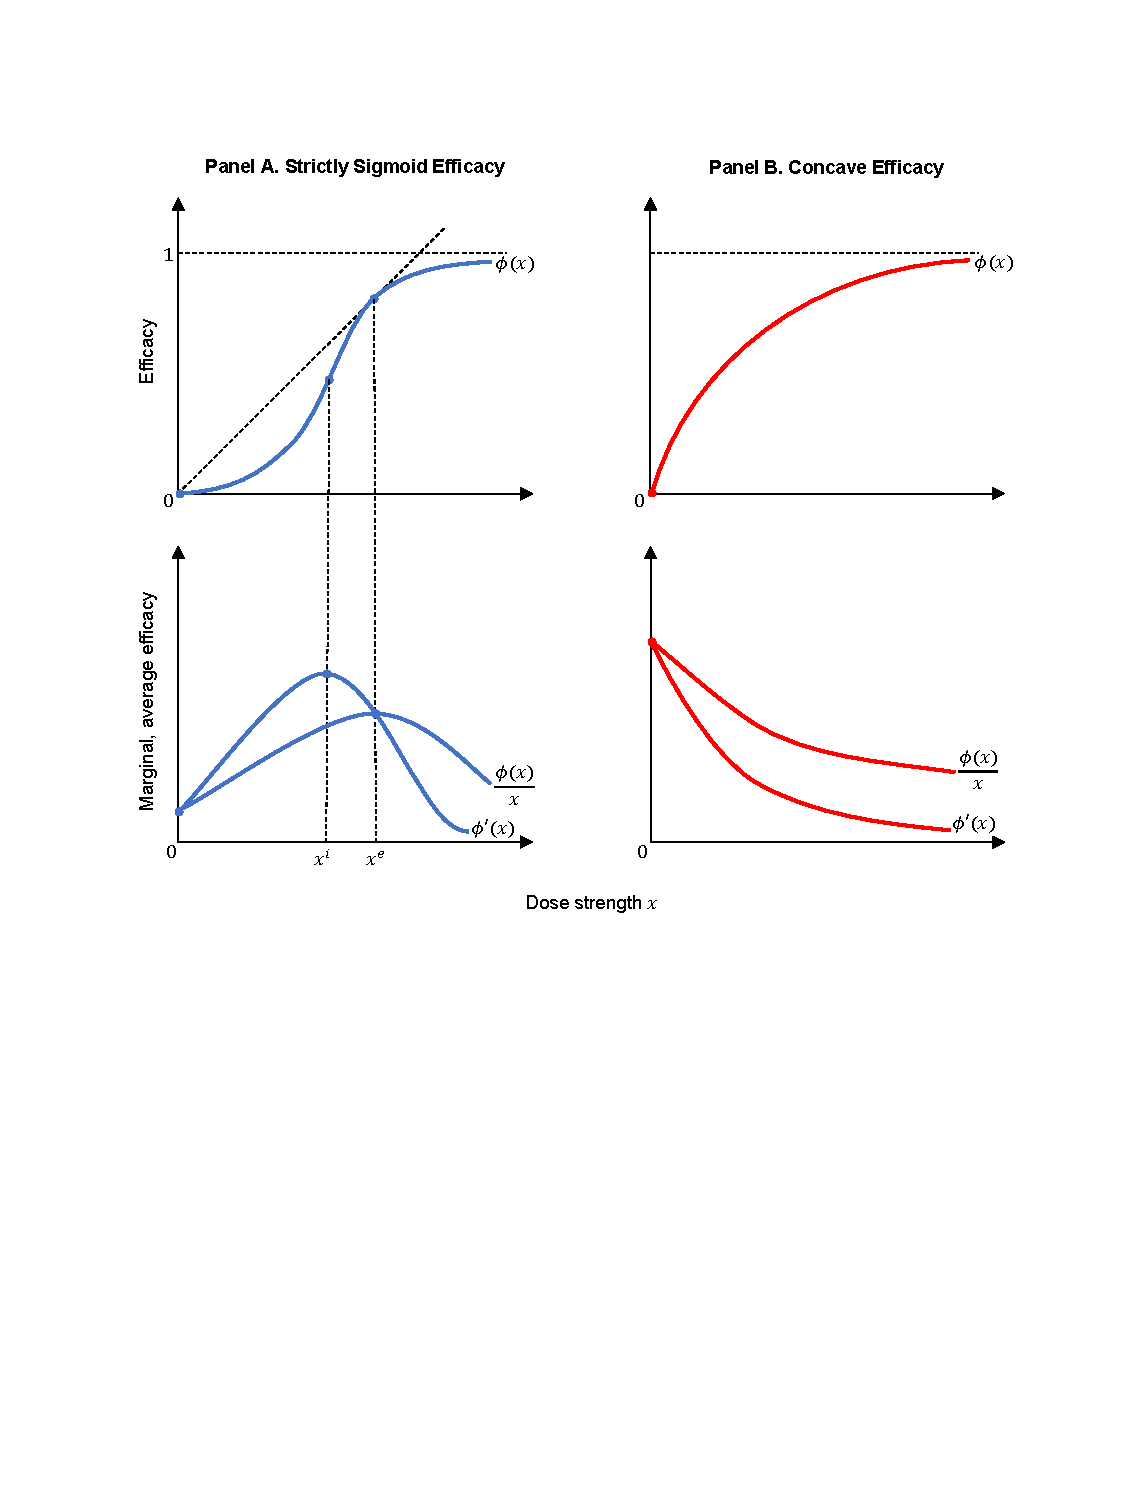
\includegraphics[viewport=65 280 495 645, width=.85\textwidth, clip]{figures/efficacy_four_panels.pdf}
\vspace{1ex}
\caption{{\bf Subcases of a Sigmoid Efficacy Function.} The panels on
  the left exhibit the case of strictly sigmoid $\efficacy$, having an
  interior inflection point $\xpoi > 0$ and interior point of unit
  elasticity, $\xunit > 0$. The panels on the right exhibit the case
  of concave $\efficacy$. A concave $\efficacy$ can equivalently be
  thought of as a weakly sigmoid curve, the first derivative of which
  has a mode at 0.}
\label{fig:efficacy}
\end{figure}

Sigmoid dose-response curves are widely used in the pharmacometric
modeling of vaccines \citep{Rhodes2022}, receiving both theoretical
and empirical support in the scientific literature. The fact that the
increase in efficacy is initially slow at low levels of the active
ingredient is consistent with threshold effects in immune
response. For example, a T-cell requires a cetain number of receptor
signals to trigger cytokine response \citep{Itoh1997} and
proliferation \citep{AnYeung2014}. That $\efficacy$ eventually
plateaus reflects the saturation of the immune system
\citep{Borghans1999} and homeostatic mechanisms such as regulatory
T-cells that prevent excessive immune responses leading to autoimmune
disease \citep{Sakaguchi2008}.\footnote{Biology aside, as a
mathematical principle, any increasing, bounded function converges to
its limit from below, implying that it must eventually plateau.}
Empirical estimates of dose-response functions find a sigmoid shape
fits the data well in both animal and human studies
\citep{deJonge2020,Roozendall2021}.

Let $\side(x) \geq 0$ denote the expected harm from side effects for
an individual vaccinated with a dose of strength $x$. We will take the
function $s : [0,\infty) \rightarrow [0,\infty)$ to be real-analytic
    on $[0,\infty)$. Assume that a vaccine with no active ingredient
      produces no side effects, i.e., $\side(0) = 0$. Assume further
      that side effects are nondecreasing in dose strength at a
      nondecreasing rate: i.e., $\side'(x) \geq 0$ and $\side''(x)
      \geq 0$ for all $x \geq 0$.

The population consists of a continuum of homogeneous individuals of
mass $N$. Letting $n \in [0,N]$ denote the mass of individuals
receiving a vaccine course and $v \in [0,N]$ denote the mass of
successfully immunized people, we have $v = n \efficacy(x)$. Denote
the social benefit from preventing disease harm via successful
vaccination by $B(v)$, capturing both the direct protective effects
and the indirect epidemiological effects of reducing transmission from
immunized individuals. While there is a natural reason to restrict the
domain of the benefits function to $[0,N]$ since successfully
vaccinating more than 100\% of the population does not have a physical
meaning, for technical reasons we will take $B : [0, \infty)
  \rightarrow [0,\infty)$ to be a real-analytic extension of the
    benefit function over the entire nonnegative real
    line.\footnote{Our specification accommodates the possibility that
    vaccinating the last person in a 100\% successful universal
    vaccination campaign has positive marginal benefit (a case that
    could arise if vaccination prevents individual harm but not
    transmission). Alternative extensions of $B$ have drawbacks. One
    alternative extension would be to set $B'(N) > 0$ but $B'(v) = 0$
    for all $v > N$. This alternative is not differentiable at $N$ and
    thus not real-analytic on $[0, N]$. Another alternative would be
    to specify $B'(v) = 0$ for all $v \geq N$, but this restricts the
    value and shape of benefits $B(v)$ in a neighborhood below $N$. We
    address the concern that extending the benefit function above $N$
    could lead to planner solutions outside of the range with physical
    meaning by including constraint $n \leq N$ in the planner's
    problem.} Normalize benefits to 0 in the absence of vaccinations,
    i.e., $\benefit(0) = 0$. Assume benefits are increasing and
    strictly concave, i.e., for all $v \geq 0$, $\benefit'(v) > 0$ and
    $\benefit''(v) < 0$. The assumption of concave benefits follows
    previous economic analyses of the market for epidemic
    vaccines. \citet{Ahuja2021} justify their use of a concave benefit
    function in their calibrations of the \covid\ pandemic on the
    grounds that prioritizing initial doses to the most vulnerable
    (aged, immunocompromised, and health workers) generates steep
    initial returns, which fall as less vulnerable people are
    vaccinated, eventually reaching a plateau as the population
    reaches herd immunity.\footnote{In their model of homogeneous
    consumers, \citet[][Proposition~7]{Goodkin-Gold2024} provide
    necessary and sufficient conditions on the disease's effective
    reproductive number for the vaccine benefits to be concave.} We
    will assume the real-analytic extension satisfies $\lim_{v
      \uparrow \infty} B'(v) = 0$.

A social planner chooses the vaccine's strength $x$ and number of
people vaccinated $n$ to maximize the population's health---the social
benefit from the vaccine less harm from side effects---net of
expenditures. The planner's expenditures include spending on the
vaccine's active ingredient (antigen), for which the planner pays an
exogenous unit price $p \geq 0$.\footnote{\label{fn:Castillo} The
choice to model $p$ as a constant, independent of the quantity
demanded by the vaccine program, can be justified on several
grounds. On theoretical grounds, price-taking is relevant to the case
in which the planner controls vaccine production and internalizes unit
cost $c$ as the relevant price $p$. Price-taking is also a reasonable
assumption if the vaccine program is only a small part of the overall
vaccine market. On practical grounds, during the Covid-19 pandemic,
vaccine manufacturers appear to have been content to ration supplies
to countries rather than letting rising prices clear the
market. \citet{Castillo2021} found that vaccine courses (generally two
doses) were being sold for between \$6 and \$40, compared to an
estimated social value in the thousands of dollars. Vaccine
manufacturers might fear that raising prices during a crisis would be
judged repugnant \citep{Kahneman1986} and generate a backlash.}  This
price may equal unit cost $c$ or may reflect a markup $m \equiv
p -c$ above $c$.

The planner also expends $k \geq 0$ per dose to administer the
vaccine, independent of the dose's strength. This includes the cost of
filling and finishing the vaccine vial, transporting the vials to
dispensaries, and labor and facilities involved in administering a
dose to a consumer. If the social planner internalizes the consumer's
cost of traveling to the dispensary and the pain of being jabbed,
those costs could be included in $k$ as well.

The planner's objective is thus to maximize the value of its objective
\begin{equation}
\label{obj}
\benefit \bigl( n\efficacy(x) \bigr) - n \left[ \side(x) + px + k
  \right].
\end{equation}
Our specification nests the case of a perfectly benevolent planner who
internalizes suppliers' profits. That case can be recovered by
substituting $p = c$ into equation \eqref{obj}, which then becomes
equivalent to social welfare. In practice, many health agencies do not
internalize firm profits, so the model is specified to allow for that
possibility.

Let $\general(x) \equiv \side(x) + px + k$ denote the planner's
generalized cost of vaccinating an individual, embodying both the
expected harm the individual experiences from side effects as well as
fixed and variable expenditures on a dose. The function $\general$
inherits several key properties of $\side$: namely, for all $x \geq
0$, it is weakly increasing, as $\general'(x) = \side'(x) + p \geq 0$;
it is convex, as $\general''(x) = \side''(x) \geq 0$; and it is
real-analytic, as its component functions are. The planner's objective
\eqref{obj} can then be rewritten more succinctly as
\begin{equation}
\label{obj_g}
\benefit \bigl( n\efficacy(x) \bigr) - n \general(x).
\end{equation}

The planner faces several constraints on this problem. Let $Q > 0$
denote the supply of the active ingredient. The total quantity used
cannot exceed this supply:
\begin{equation}
\label{capacity}
nx \leq Q.
\end{equation}
Further, no more than the total population can be vaccinated:  
\begin{equation}
\label{population}
n \leq N.
\end{equation}
Finally, the planner's choice variables must be nonnegative:
\begin{equation}
n, x \geq 0. \label{pos} 
\end{equation}

As usual, elasticities will play a key role in the analysis. Let
$\elasticity{f}(x) \equiv x f'(x) / f(x)$ denote the elasticity of an
arbitrary function $f$ at point $x$. In particular,
$\elasticity{\efficacy}\!(x)$ is the elasticity of efficacy at dosage
$x$ and $\elasticity{\general}\!(x)$ is the elasticity of generalized
marginal cost. It will also be useful to have notation for a
function's per-unit average, $\perunit{f}(x) \equiv f(x) / x$. In
particular, $\perunit{\efficacy}\!(x)$ is the per-unit efficacy of
dosage $x$ and $\perunit{\general}\!(x)$ is the per-unit generalized
cost.

%%%%%%%%%%%%%%%%%%%%%%%%%%%%%%%%%%%%%%%%%%%%%%%%%%%%%%%%%%%%%%%%%%%%%%%%%%%%%%%

\Section{Optimal Dosing with Costless Vaccination}
\label{s:Costless}

We begin the analysis by abstracting from any costs of vaccination,
setting $\general(x) = 0$. This is a good place to begin for several
reasons. First, the analysis in this case is relatively simple and
generates clear results on fractional dosing. Second, this is the case
carried into the calibrations for the \covid\ pandemic in
Section~\ref{s:Calibrations}. That section derives the social benefit
of vaccination from a complex epidemiological model and calibrates
various functional forms for the efficacy function based on data for
\covid\ vaccines. However, that section takes a cruder approach to
costs, setting $g(x) = 0$, in part because of a paucity of information
on costs but mainly reflecting our view that the social costs of
vaccination were eclipsed by the social benefits in the
\covid\ pandemic (see footnote~\ref{fn:Castillo}).

%------------------------------------------------------------------------------

\SubSection{Unit-Elastic Benchmark}
\label{ss:Elasticity}

The key benchmark with costless vaccination is provided by the dosage
$\xunit$ at which efficacy is unit elastic. First suppose $\efficacy$ is concave. We have
\begin{equation}
\label{lHopital}
\lim_{x \downarrow 0} \elasticity{\efficacy}(x) = \lim_{x \downarrow 0} \frac{x \efficacy'(x)}{\efficacy(x)} = \frac{\efficacy'(0) + 0 \cdot \efficacy''(0)}{\efficacy'(0)} = 1, 
\end{equation}
where the first equality is definitional, the second is an application of l'H\^{o}pital's Rule, and the last uses the fact that $\efficacy'(0) > 0$ for concave $\efficacy$. 
While $\elasticity{\efficacy}\!(x)$ is undefined at $x=0$, having the $0/0$ form, it is natural to extend this function to equal its right-hand limit at 0: thus,
$\elasticity{\efficacy}\!(0) = 1$. According to this definition, the origin is a point of unit elasticity for concave $\efficacy$, and we later verify this is the only such point for this functional form.

For strictly sigmoid $\efficacy$, the origin may or may not be a point of unit elasticity.\footnote{The origin is guaranteed to be a point of unit elasticity for strictly sigmoid $\efficacy$ if $\efficacy'(0) > 0$ but need not be if $\efficacy'(0) = 0$. For example, the limiting elasticity for the strictly sigmoid function $\efficacy(x) = 1 - \exp(-x^2)$ is $\lim_{x \downarrow 0} \elasticity{\efficacy}(x) = 2$.} It is guaranteed to be unit elastic at a different point---the interior point where the chord from the origin is
tangent to the curve (see Figure~\ref{fig:efficacy}). The analysis will focus on this nontrivial
unit-elastic point when possible but settle for the trivial point $0$
when $\efficacy$ is concave and has no positive unit-elastic point,
as the following definition reflects:
\begin{equation}
\label{xunit}
\xunitbar \equiv \max \left\{ x \geq 0 \mid
\elasticity{\efficacy}\!(x) = 1 \right\}.
\end{equation} 

The following lemma states that $\xunitbar$ is well defined and
characterizes additional of its useful properties. The proofs of this
and all subsequent results are provided in the appendix.
\begin{lemma}
\label{l:xunit}
\singlespace
There exists a unique $\xunitbar \geq 0$ satisfying equation
\eqref{xunit}. When $\efficacy$ is strictly sigmoid, $\xunitbar >
\xpoi > 0$; when $\efficacy$ is concave, $\xunitbar = 0$. By
definition, $\elasticity{\efficacy}\!(\xunitbar) = 1$. For all $x \in
(0, \xunitbar)$, $\elasticity{\efficacy}(x) > 1$; for all $x >
\xunitbar$, $\elasticity{\efficacy}(x) < 1$.
\end{lemma}

The unit-elastic dosage $\xunitbar$ provides a key benchmark for the
analysis. As the next lemma states, $\xunitbar$ maximizes per-unit
efficacy, $\perunit{\efficacy}\!(x) \equiv \efficacy(x) / x$, which will figure into the optimal policy when vaccination is costless.
\begin{lemma}
\label{l:a}
\singlespace
Per-unit efficacy $\perunit{\efficacy}\!(x)$ is strictly
quasiconcave. It is strictly increasing for $x \in (0, \xunitbar)$,
strictly decreasing for $x > \xunitbar$, and reaches a maximum at
$\xunitbar$.
\end{lemma}

\noindent The relatively lengthy proof using only basic mathematics is
supplemented with a shorter alternative leveraging a result in
\citet{Karlin1956} that certain integral transforms of a function have
a variation-diminishing property, experiencing no more sign changes
than the function itself.

%------------------------------------------------------------------------------

\SubSection{Optimal Vaccine Program}
\label{ss:Optimum_Costless}

With the analysis of the unit-elastic benchmark $\xunitbar$ in hand, we
can proceed to solve for the planner's optimum.  Substituting
$\general(x) = 0$ into equation \eqref{obj_g}, with costless
vaccination the objective function simplifies to
\begin{equation}
\label{obj_costless}
\benefit \bigl( n\efficacy(x) \bigr). 
\end{equation}

It is evident that capacity constraint \eqref{capacity} binds so all
capacity $Q$ is used in an optimum. For any policy $(n,x)$ that does
not exhaust capacity, it can be improved upon by using some of the
residual capacity to vaccinate the same individuals with a stronger
dose. Stronger doses increase social benefits since $\efficacy(x)$ and
$\benefit(v)$ are increasing in their arguments but entail no greater
social costs.

We thus have $n^* x^* = Q$. Rearranging this equation as $n^* = Q /
x^*$ and substituting into \eqref{obj_costless} yields $\benefit
\bigl( Q \efficacy(x^*) / x^* \bigr) = \benefit \bigl( Q
\perunit{\efficacy}\!(x^*) \bigr)$. Since $\benefit$ is increasing in
its argument and $Q$ is a constant, we see that the $x^*$ should
maximize per-unit efficacy $\perunit{\efficacy}\!(x)$ and thus equal
$\xunitbar$ by Lemma~\ref{l:a}. This is the optimal dose unless unless it
would leave some capacity unused even if all $N$ individuals were
vaccinated with it. In that case, the optimum simply vaccinates the
entire population ($n^* = N$) with the largest possible dose subject
to available capacity ($x^* = Q/N$). The following proposition
synthesizes this analysis.
\begin{proposition}
\label{p:costless}
\singlespace
Suppose vaccination is costless to the planner, i.e., $\general(x) =
0$. The optimal policy vaccinates $n^* = \min \{ Q/\xunitbar, N \}$
individuals with dose $x^* = \max \{ \xunitbar, Q/N \}$.
\end{proposition}

The optimal policy can be visualized with the help of
Figure~\ref{fig:costless_optimum}. Focus first on the top panel,
covering the subcase of strictly sigmoid $\efficacy$. Given
vaccination is costless and benefits and efficacy do not hit peaks,
there is no largest optimal dose. For very high levels of capacity
$Q$, the optimal dose vaccinates the whole population with the largest
possible dose allowed by available capacity: $x^* = Q/N$. No matter
how high $Q$ is, there is a sense in which the optimal dose is still ``fractional'' in that it is smaller than the optimal dose would be with more capacity. In this sense, fractional dosing is the rule, not the exception.

\begin{figure}[tp]
\centering
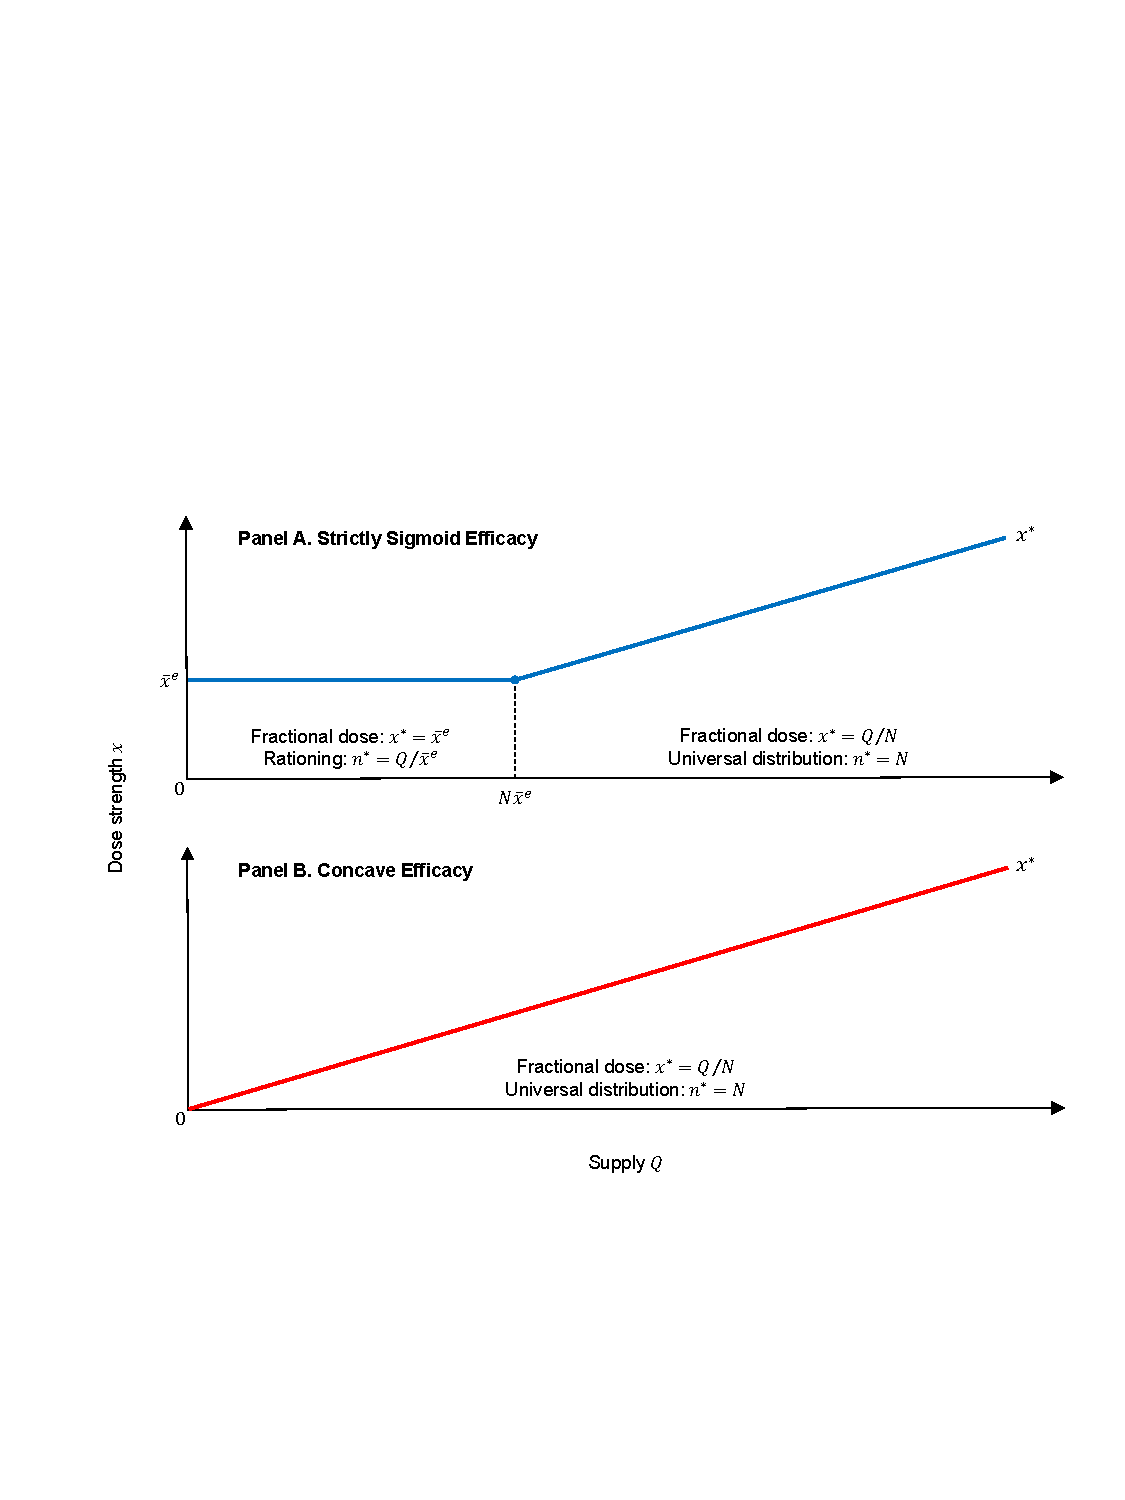
\includegraphics[viewport=50 155 530 475, width=.9\textwidth, clip]{figures/costless_optimum.pdf}
\vspace{1ex}
\caption{{\bf Optimal Dosage with Costless Vaccination.} The panels
  show the planner's optimal vaccine policy for different shapes of a
  sigmoid efficacy function, strictly sigmoid in the top panel and
  concave in the bottom panel.}
\label{fig:costless_optimum}
\end{figure}

As capacity shrinks from some initial high level, the optimal dose
falls linearly until a kink is hit at $Q = N \xunitbar$. Below that
threshold capacity, rather than continuing to shrink the size of the
dose linearly, it is better for population health to keep the dose at
the level $\xunitbar$ maximizing per-unit efficacy and ration it in
the population. The unit-elastic dose $\xunitbar$ provides a floor on
optimal dose size.

The lower panel covers the subcase of concave $\efficacy$. In that
subcase, $\xunitbar = 0$, so the unit-elastic dose does not provide a
floor on optimal dose size. Population health is maximized by
spreading available capacity evenly in the population. Thus, the
optimal dose continues to shrink linearly with capacity $Q$ all the
way to the origin.

A formal proof of Proposition~\ref{p:costless} is provided in the
appendix. The planner's problem of choosing $x$ and $n$ to maximize
objective \eqref{obj_costless} subject to inequality constraints
\eqref{capacity}--\eqref{pos} can be solved using the
Karush--Kuhn--Tucker (KKT) method. In the appendix, we prove that the
problem satisfies linear independence constraint qualification (LICQ),
a textbook condition ensuring the KKT conditions are necessary for an
optimum \citep{Solodov2011}. The KKT conditions narrow the optimum
down to two potential solutions---an interior solution involving
unit-elastic dose $\xunitbar$ and a corner solution---which can be
compared. The interior solution solves the relaxed problem omitting a
constraint and thus provides the optimum in the original problem
unless it violates the omitted constraint, in which case the corner
solution provides the optimum.

%%%%%%%%%%%%%%%%%%%%%%%%%%%%%%%%%%%%%%%%%%%%%%%%%%%%%%%%%%%%%%%%%%%%%%%%%%%%%%%

\Section{Optimal Dosing with Costly Vaccination}
\label{s:Costly}

In the case of costless vaccination just studied, there is no reason
not to use all available capacity, so the capacity constraint
\eqref{capacity} always binds. This reduces the complexity of the
optimal policy. As the first panel of Figure~\ref{fig:matrices}
indicates, the optimal policy can take one of only two forms depending
on whether the remaining constraint---the population constraint
\eqref{population}---binds. If the population constraint does not
bind, the optimal solution is interior, involving the unit-elastic
dose $\xunitbar$; if the population constraint bids, the two variables in
the optimal policy $n^*$ and $x^*$ are exactly determined by the two
equations provided by the binding constraints.

\begin{figure}[tp]
\centering
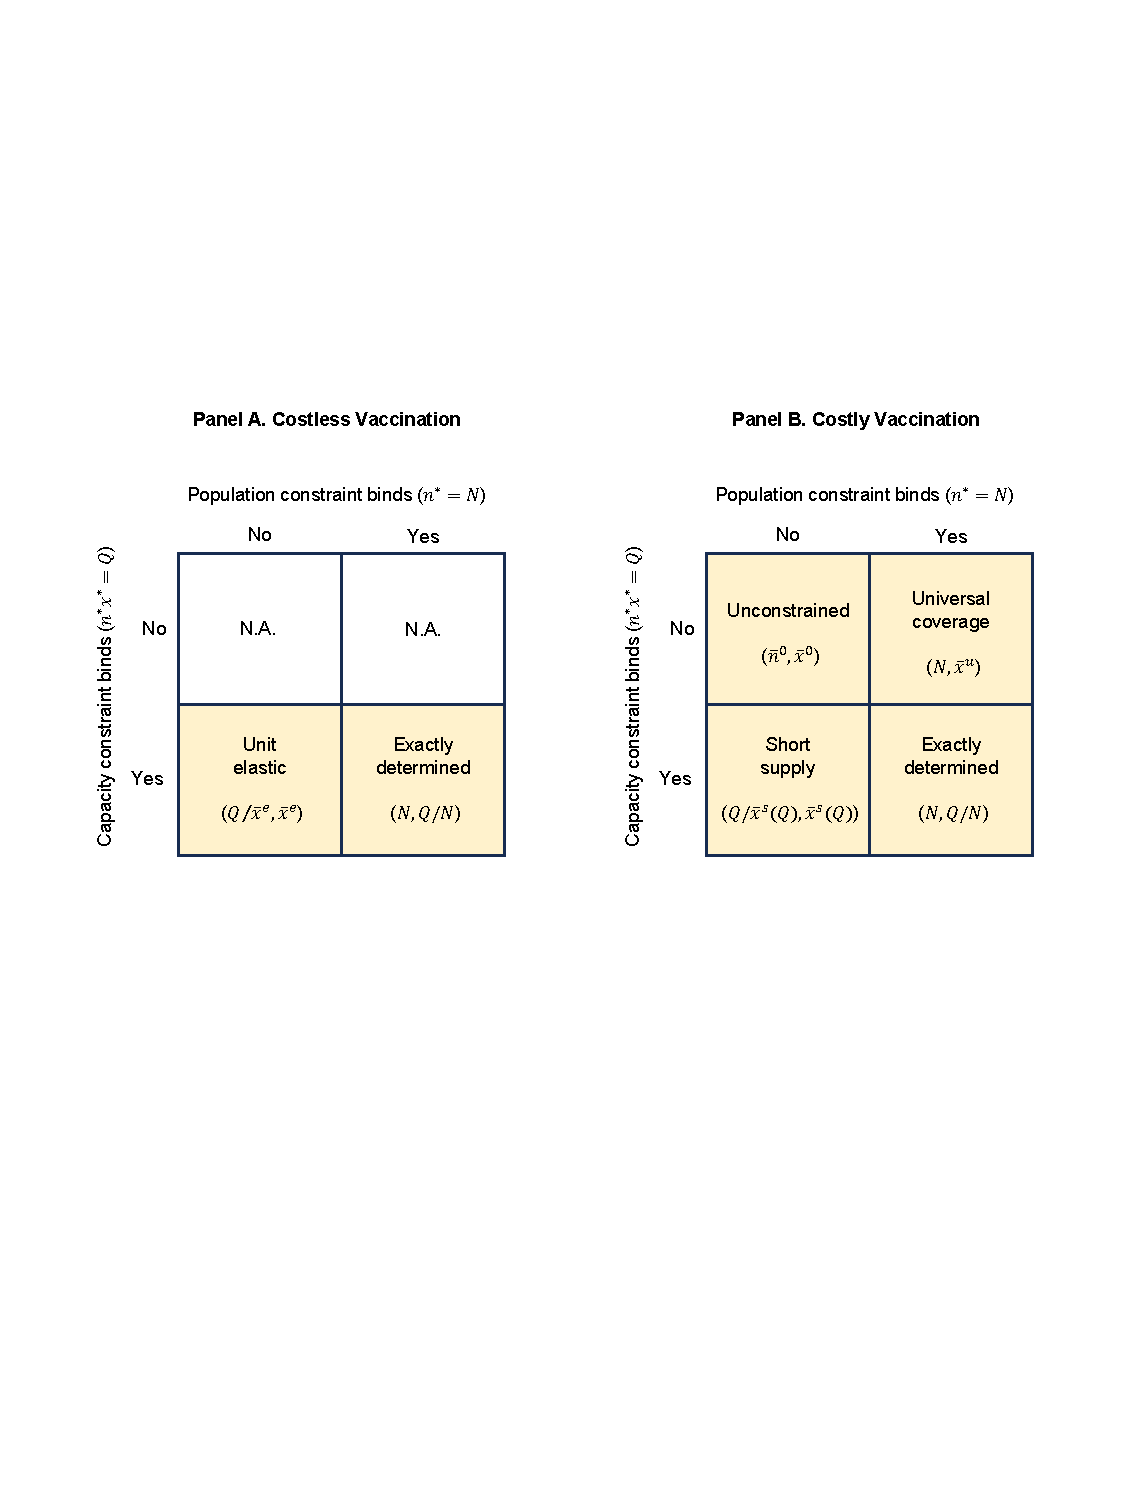
\includegraphics[viewport=45 305 500 525, width=.9\textwidth, clip]{figures/matrices.pdf}
\vspace{1ex}
\caption{{\bf Benchmarks Comprising Optimal Solution.} The planner's
  optimum, solved using the KKT method, is comprised of the benchmarks
  in the matrix entries, each characterized in a subsequent
  subsection.}
\label{fig:matrices}
\end{figure}

This section studies the case of costly vaccination, assuming $p,k >
0$ and $\side(x) \geq 0$, implying $\general(x) > 0$ for all $x >
0$. Now there is a reason not to use all available capacity. The
decreasing marginal social benefit of employing the last units of
capacity may not justify the increasing marginal social cost. The
optimal policy becomes more complex, taking on four possible forms
delineated in the second panel of Figure~\ref{fig:matrices}, depending
on whether capacity constraint and/or the population constraint
bind. Each of the four boxes provides a benchmark characterized in a
series of subsections below. These benchmarks become building blocks
in constructing the planner's optimum, derived using the KKT method.

%------------------------------------------------------------------------------

\SubSection{Nontrivial Policy}
\label{ss:Nontrivial_Sigmoid}

With costless vaccination, the optimal policy is always nontrivial,
i.e., involving positive vaccinations ($n^* > 0$) and positive dosage
($x^* > 0$). Indeed, it is optimal to allocate the whole capacity $Q$
across some or all individuals in the population. By contrast, the
optimal policy may be trivial with costly vaccination---namely when
the cost of every nontrivial vaccine policy exceeds its benefit. The
following lemma provides a necessary and sufficient condition for a
nontrivial optimum under costly vaccination.
\begin{lemma}
\label{l:nontrivial_generic}
\singlespace
The planner's optimum is nontrivial if and only if $\benefit'(0)
\efficacy(x) > \general(x)$ for some $x > 0$.
\end{lemma}

To gain some intuition for the proof of the lemma, suppose $B'(0)
\efficacy(x) > \general(x)$ for some $x > 0$. Then a policy of
vaccinating a few people with that dosage generates a greater health
benefit than generalized cost. This policy thus provides the planner
with positive surplus, strictly dominating the trivial policy of not
vaccinating anyone. On the other hand, suppose $B'(0) \efficacy(x)
\leq \general(x)$ for all $x > 0$. Then there is no way for the
planner to obtain positive surplus by vaccinating a few
people. Vaccinating more people would be even worse for the planner
because the benefit function $B$ is concave. So the trivial policy of
not vaccinating anyone is optimal in that case.

The condition for a nontrivial optimum stated in
Lemma~\ref{l:nontrivial_generic} is rather amorphous and may be
difficult to verify. We can provide a more pointed, equivalent
condition; but since it requires notation developed in the next
subsection, we postpone its statement until then.

%------------------------------------------------------------------------------

\SubSection{Unconstrained Benchmark}
\label{ss:Unconstrained}

The first benchmark we analyze involves maximizing the planner's
objective \eqref{obj_g} removing the capacity and population
constraints, retaining only the nonnegativity constraints:
\begin{equation}
\label{hats}
\max_{n,x \geq 0} \left[ \benefit \! \bigl( n \efficacy(x) \bigr) - n
  \general(x) \right].
\end{equation}
Denote the solution by $(\nno, \xno)$. In this subsection, we provide
a characterization of this solution and show it is well defined under
the condition in Lemma~\ref{l:nontrivial_generic} ensuring the
planner's optimum is nontrivial.

Considerable insight can be gained by examing the problem that is
equivalent to \eqref{hats} but makes the change of variables $v = n
\efficacy(x)$ and solves for the optimal number of successful
immunizations $v$ rather than the optimal number of vaccinations
$n$. Equation \eqref{hats} becomes
\begin{equation}
\label{hats2}
\max_{v,x \geq 0} \left[ \benefit(v) - v \cdot
  \frac{\general(x)}{\efficacy(x)} \right].
\end{equation}

It is immediate that the unconstrained-optimal dose $\xno$ maximizes
the ratio $\efficacy(x) / \general(x)$. This ratio is not guaranteed
to have a unique maximizer (though it will in many applications). Let
$\Xno$ denote the set of maximizers,
\begin{equation}
\label{max_ratio}
\Xno \equiv \argmax_{x \geq 0} \left[
  \frac{\efficacy(x)}{\general(x)} \right],
\end{equation}
and $\xno$ be an arbitrary element of $\Xno$. The analysis will often
focus on the largest maximizer: $\xnobar \equiv \max(\Xno)$. The
largest maximizer forms a solution pair $(\nnobar, \xnobar)$ most
likely to respect the omitted constraints and thus provide a feasible
solution to the unconstrained problem (a detail covered in the
relevant appendix proof).

Taking the first-order condition with respect to $x$ in equation
\eqref{max_ratio} and rearranging yields a necessary condition for any
maximizer $\xno$:
\begin{equation}
\label{equal_elasticities}
\elasticity{\efficacy}(\xno) = \elasticity{\general}(\xno). 
\end{equation}
The optimal dose in the unconstrained problem balances the percentage
increase in efficacy against the percentage increase in generalized
cost entailed by a dose increase. Note that the social benefit
generated by the vaccine does not appear in this equation, only its
efficacy. Below, we will see that the social benefit factors into the
determination of the optimal number of vaccinations $\nno$, but the
optimal dose they are vaccinated with only depends on efficacy and
generalized cost.

The preceding sketch of the analysis glossed over some technical
details. It remains to be verified that $\Xno$ is nonempty and finite
so that its largest element $\xnobar$ is well defined. The following
lemma fills in those technical details. It also provides a useful
result, positioning $\xnobar$ relative to the unit-elastic benchmark
$\xunitbar$: if $\xnobar \geq \xunitbar$, then $\Xno$ is a singleton. This
result follows since if any solution $\xno$ lies above $\xunitbar$, it
lies above the point of inflection for $\efficacy$, in the range where
$\efficacy$ is a well-behaved concave function, generating a unique
optimum.
\begin{lemma}
\label{l:xno}
\singlespace
There exists a unique $\xnobar > 0$ satisfying $\xnobar =
\max(\Xno)$. If $\xnobar \geq \xunitbar$, then $\Xno = \{ \xnobar \}$.
\end{lemma}

The ratio of the social benefit to cost of vaccinating the $n$th
individual with the unconstrained optimal dose $\xnobar$ will play an
important role in the subsequent analysis, so we introduce notation
for it:
\begin{equation}
\label{BCR}
\ratio(n) \equiv \frac{\benefit' \! \bigl( n \efficacy(\xnobar) \bigr)
  \efficacy(\xnobar)}{\general(\xnobar)}.
\end{equation} 
When $\ratio(n) > 1$, a case can be made for vaccinating the $n$th
person---at least in a counterfactual unconstrained world. The
inequality tells us that the social benefit exceeds the cost of
vaccinating the $n$th person with the dose $\xnobar$ that, like all
elements of $\Xno$, has the greatest potential to generate higher
benefits than costs. That is not to say that $\xnobar$ will be the
optimal dose when supply and population constraints operate or that
vaccinating the $n$th person will be optimal then. The inequality
provides a necessary but not sufficient condition for the $n$th person
to be vaccinated in the planner optimum. When $\ratio(n) \leq 1$, on
the other hand, vaccinating the $n$th person cannot be strictly
optimal.

The derivative of \eqref{BCR} with respect to $n$ is 
\begin{equation}
\label{dBCR}
\frac{\benefit'' \! \bigl( n \efficacy(\xnobar) \bigr)
  \efficacy(\xnobar)^2}{\general(\xnobar)},
\end{equation}
which is negative since $\benefit'' < 0$. This negative derivative
implies that the case for vaccinating the next individual is
increasingly hard to make as more individuals are vaccinated. The
marginal social cost of vaccinating each individual remains the same
but the marginal social benefit falls.

We can put this notation to immediate use in restating the condition
for a nontrivial planner optimum more succinctly.
\begin{lemma}
\label{l:nontrivial}
\singlespace
The planner's optimum is nontrivial if and only if $\ratio(0) > 1$.
\end{lemma}

\noindent Intuitively, if $\ratio(0) > 1$, a case can be made for
vaccinating a few individuals with dose $\xnobar$. Whatever the
available supply and whatever the dosage, there is always enough to
vaccinate a sufficiently small number of individuals with that
dosage. If $\ratio(0) \leq 1$, on the other hand, it is not socially
worthwhile to vaccinate even the first individual, let alone an
individual added to the $n$ that have already been vaccinated.

It remains to derive $\nno$. Substituting $\xno$ into \eqref{hats2}
and taking the first-order condition with respect to $v$ yields
$\benefit' \!(\vno) = \general(\xno) / \efficacy(\xno)$. Changing back
to the original choice variables, $\vno = \nno \efficacy(\xno)$, and
solving for $\nno$ yields
\begin{equation}
\label{nno}
\nno = \frac{1}{\efficacy(\xno)} (\benefit')^{-1} \! \left(
\frac{\general(\xno)}{\efficacy(\xno)} \right).
\end{equation}
If the planner's optimum is nontrivial, it can be shown that the
inverse $(B')^{-1}$ exists and thus equation \eqref{nno} has a
solution, as the next lemma states.
\begin{lemma}
\label{l:nno}
\singlespace
As long as the planner's optimum is nontrivial, there exists a unique
$\nno > 0$ satisfying \eqref{nno}.
\end{lemma}

When $\Xno$ includes several maximizers, different $\xno \in \Xno$
pair with different $\nno$ solving equation \eqref{nno}. In
particular, larger $\xno$ are associated with smaller
$\nno$.\footnote{To see this, note that the ratio in the argument of
$(\benefit')^{-1}$ is independent of which $\xno$ is selected because
all of them maximize the ratio $\efficacy(x)/\general(x)$, but the
leading factor $1 / \efficacy(\xno)$ is decreasing in $\xno$.} Let
$\nnobar$ denote the solution to equation \eqref{nno} when $\xno =
\xnobar$.

%------------------------------------------------------------------------------

\SubSection{Universal-Coverage Benchmark}
\label{ss:Universal}

We next analyze what we call the universal-coverage benchmark,
maximizing the planner's objective \eqref{obj_g} given the entire
population must be vaccinated:
\begin{equation}
\label{max_xuniv}
\max_{x \geq 0} \left[ \benefit \! \bigl( N \efficacy(x) \bigr) - N
  \general(x) \right].
\end{equation}

As before,
the maximizer of this objective is not guaranteed to
be unique. Let $\Xuniv$ denote the set of maximizers,
\begin{equation}
\label{argmax_xuniv}
\Xuniv \equiv \argmax_{x \geq 0} \left[ \benefit \! \bigl( N
  \efficacy(x) \bigr) - N \general(x) \right],
\end{equation}
and $\xuniv$ denote an arbitrary element of $\Xuniv$. While we focused
on the largest maximizer in the previous benchmark, here we will
switch the focus to the smallest maximizer $\xunivlbar \equiv \min(
\Xuniv )$. The smallest maximizer relaxes the omitted capacity
constraint to the extent possible and thus is the most likely
maximizer to constitute a feasible solution.

It is not a foregone conclusion that the objective function
\eqref{max_xuniv} has a nontrivial maximizer and if there is a set of
maximizers, that this set is finite so has a well-defined largest
element. The next lemma provides a condition guaranteeing these
conclusions are true.
\begin{lemma}
\label{l:xuinv}
\singlespace
If $\ratio(N) \geq 1$, there exists a unique $\xunivlbar > 0$
satisfying $\xunivlbar = \min(\Xuniv)$.
\end{lemma}
\noindent The proof, while similar to that of Lemma~\ref{l:xno}, is
not identical, so we provide a separate proof in the appendix.

Taking the first-order condition and rearranging, we have that any
maximizer $\xuniv$ must satisfy
\begin{equation}
\label{foc_xuniv}
\benefit' \! \bigl( N \efficacy(\xuniv) \bigr) \efficacy'(\xuniv) =
g'(\xuniv).
\end{equation}
The left-hand side is the marginal social benefit (per vaccinated
individual) of increasing dose strength. The optimal dose in the
universal-coverage benchmark equates this marginal social benefit with
the marginal generalized cost of that dosage increase on the
right-hand side of the equation.

%------------------------------------------------------------------------------

\SubSection{Short-Supply Benchmark}
\label{ss:Short}

The next benchmark is the mirror image of the one just analyzed. The
universal-coverage benchmark maximized the planner's objective
omitting the constraint on supply $Q$, fixing the number of people to
be vaccinated $N$. The benchmark analyzed here drops the constraint on
the number of vaccinations and instead fixes the supply of vaccine
substance that must be utilized at $Q$. We will call this the
short-supply benchmark. The label anticipates the role this benchmark
will play in the planner's optimum, providing the formula for the
optimum when supplies $Q$ become so tight that the supply constraint
\eqref{capacity} takes over as the only active constraint; supplies
are too constrained to consider vaccinating anywhere near the total
population, allowing us to safely ignore constraint \eqref{population}
on the number of vaccinations.

The binding constraint that $Q$ must be fully utilized entails $n x =
Q$. Substituting $n = Q/x$ into the planner's objective function
\eqref{obj_g}, the maximization problem can be written
\begin{equation}
\label{max_xshort}
\max_{x \geq 0} \left[ \benefit \! \bigl( Q \perunit{\efficacy}\!(x)
  \bigr) - Q \perunit{\general}\!(x) \right].
\end{equation}
Let $\Xshort\!(Q)$ denote the set of maximizers,
\begin{equation}
\label{argmax_xshort}
\Xshort\!(Q) = \argmax_{x \geq 0} \left[ \benefit \! \bigl( Q
  \perunit{\efficacy}\!(x) \bigr) - Q \perunit{\general}\!(x) \right],
\end{equation}
and $\xshort\!(Q) \in \Xshort\!(Q)$ denote an arbitrary maximizer. For
this benchmark, the analysis will focus on the largest maximizer,
$\xshortbar\!(Q) \equiv \max [ \Xshort\!(Q) ]$, since this relaxes the
omitted population constraint to the extent possible and thus is the
most likely maximizer to constitute a feasible solution. We have
emphasized the dependence of these maximizers on $Q$ by adding it as
an argument; benchmarks analyzed in previous subsections did not
include a supply constraint, so those benchmark optima are independent
of $Q$.

If $Q$ is large, there is no guarantee forcing the population to
consume that much vaccine substance will generate positive surplus. If
$Q$ is sufficiently small, however, allocating that supply to the
population in doses of size $\xshortbar\!(Q)$ is guaranteed to
generate positive surplus if the planner's optimum is nontrivial, as
the next lemma states.
\begin{lemma}
\label{l:xshort}
\singlespace
Suppose the planner's optimum is nontrivial. For sufficiently small $Q
> 0$, there exists a unique $\xshortbar\!(Q) > 0$ satisfying
$\xshortbar\!(Q) = \max[\Xshort\!(Q)]$ and delivering a positive value
of the objective \eqref{max_xshort}.
\end{lemma}

Taking the first-order condition in equation \eqref{max_xshort} and
rearranging, all solutions $\xshort\!(Q)$ must satisfy
\begin{equation}
\label{foc_xshort}
\benefit' \! \bigl( Q \perunit{\efficacy}\!(\xshort\!(Q)) \bigr)
\perunit{\efficacy}'\! \bigl( \xshort\!(Q) \bigr) =
\perunit{\general}' \! \bigl( \xshort\!(Q) \bigr).
\end{equation}
This rearranged first-order condition resembles the analogous one for
the universal-coverage benchmark in \eqref{foc_xuniv}. Without a
constraint on supplies, there, the planner compared marginal efficacy
to marginal generalized cost {\em in level terms}. Here, the fixed
supply ($Q$) forces the planner to compare marginal efficacy to
marginal generalized cost {\em in per-unit terms}, as the inclusion of
the factors $\perunit{\efficacy}' \!(x)$ and
$\perunit{\general}'\!(x)$ suggests.

It is natural to think that a reduction in $Q$ would reduce
$\xshortbar\!(Q)$: a tighter supply constraint would be accommodated
by smaller fractional doses. In fact, the comparative-statics is more
complicated: $\xshortbar\!(Q)$ may be increasing, constant, or
decreasing in $Q$. The next proposition provides a sufficient
statistic for the direction of the comparative-static effect,
depending on whether generalized cost is more or less elastic than
efficacy where efficacy is unit elastic. We use $\sgn(x)$ to denote the signum function, equal to $-1$ for $x<0$, $0$ for $x=0$, and $1$ for $x>0$. 
\begin{proposition}
\label{p:xshort}
\singlespace
$\sgn \bigl( d \xshortbar\!(Q) /d Q \bigr) = \sgn
\bigl( \elasticity{\efficacy}\!(\xunitbar) -
\elasticity{\general}\!(\xunitbar) \bigr) = \sgn \bigl( 1 -
\elasticity{\general}\!(\xunitbar) \bigr)$.
\end{proposition}

We have accorded this comparative-static result the status of a
proposition since, as we will see in the next subsection, it dictates
the shape of the overall planner optimum at low levels of $Q$. It is
therefore worth developing some intuition this result. Note that no
matter how the planner responds to a reduction in $Q$---whether
reducing $n$, $x$, or both---it cannot prevent the level of effective
vaccination $v$ from falling when $Q$ falls, leading to an increase in
marginal benefit $\benefit' \! (v)$ since $\benefit$ is concave. This
inclines the planner to wring more efficacy out of the limited supply
by moving the dose toward the unit-elastic point $\xunitbar$, which
maximizes per-unit efficacy, $\perunit{\efficacy}\!(x)$. Under severe
capacity constraints, the planner is willing to accept greater
marginal harm to vaccinated individuals to avoid an even greater
reduction in the social benefit of effective vaccinations. Whether
moving toward $\xunitbar$ entails an increase or decrease in $x$
depends on whether $\xshortbar\!(Q)$ is greater or less than
$\xunitbar$, which in turn depends on the relative elasticities of
$\general$ and $\efficacy$. When $\elasticity{\general}\!(\xunitbar) >
\elasticity{\efficacy}\!(\xunitbar)$, the benchmark dose
$\xshortbar\!(Q)$ is kept below the unit-elastic point $\xunitbar$ to
avoid generating too much marginal harm. In this case, moving
$\xshortbar\!(Q)$ toward $\xunitbar$ entails an increase in dose size,
explaining the surprising comparative-static result.

If $\elasticity{\general}\!(\xunitbar) <
\elasticity{\efficacy}\!(\xunitbar)$, then $\xshortbar\!(Q) >
\xunitbar$. In that case, moving $\xshortbar\!(Q)$ toward $\xunitbar$
in response to a reduction in $Q$ entails a decrease in dose size, the
anticipated comparative-static result. In the edge case where
$\elasticity{\general}\!(\xunitbar) =
\elasticity{\efficacy}\!(\xunitbar)$, $\xshortbar\!(Q) = \xunitbar$,
where it remains as $Q$ falls.

In a variety of important cases, it is straightforward to bound
$\elasticity{\general}\!(\xunitbar)$ and make definitive claims about
when the surprising comparative-static result emerges.
\begin{proposition}
\label{p:concave}
\singlespace
Suppose $\efficacy$ is concave. Then $d \xshortbar\!(Q) /
d Q > 0$.
\end{proposition}

\begin{proposition}
\label{p:linear}
\singlespace
Suppose the side-effect function is linear, i.e., $\side(x) = \sigma
x$ for some $\sigma \geq 0$. Then $\partial \xshortbar\!(Q) / \partial
Q > 0$.
\end{proposition}

\noindent The proofs of these two propositions are almost immediate
from Proposition~\ref{p:xshort}. To see the first result, if
$\efficacy$ is concave, then $\xunitbar = 0$ by
Lemma~\ref{l:xunit}. Then $\elasticity{\general}\!(\xunitbar) =
\elasticity{\general}\!(0) = 0 / k = 0$. Therefore, $1 -
\elasticity{\general}\!(\xunitbar) = 1 > 0$, implying $d
\xshortbar\!(Q) / d Q > 0$ by Proposition~\ref{p:xshort}. To see the
second result, if $\side(x) = \sigma x$, then $1 -
\elasticity{\general}\!(\xunitbar) = k / \general(\xunitbar)$, which
is positive for all $k > 0$, implying implying $d \xshortbar\!(Q) / d
Q > 0$ by Proposition~\ref{p:xshort}.

According to Propositions~\ref{p:concave} and \ref{p:linear}, the
surprising comparative-static result $\partial \xshortbar\!(Q) /
\partial Q < 0$ never emerges when $\efficacy$ is concave or
$\side(x)$ is linear. Evidently, the complex interplay between the
strictly sigmoid shape of $\efficacy$ and the convexity of $\side(x)$
is key to generating the surprising result.

When $\side(x)$ is strictly convex, the sign of $d
\xshortbar\!(Q) / d Q$ can be tied to the level of the fixed
vaccination cost, $k$.
\begin{proposition}
\label{p:k}
\singlespace
Suppose the side-effect function is strictly convex, i.e., $\side''(x)
> 0$ for all $x > 0$. Then
\begin{equation}
\label{sign_k}
\sgn \left( \frac{d \xshortbar\!(Q)}{d Q} \right) = \sgn
(k - \hat{k}),
\end{equation}
where $\hat{k} \equiv \xunitbar \side'(\xunitbar) -
\side(\xunitbar)$. If $\efficacy$ is concave, then $\hat{k} = 0$; if
$\efficacy$ is strictly sigmoid, then $\hat{k} > 0$.
\end{proposition}

\noindent The proof is again almost immediate from
Proposition~\ref{p:xshort}. Using the expression for $\hat{k}$ from
the statement of the proposition, for any $\side(x)$, we can write $1
- \elasticity{\general}\!(\xunitbar) = (k - \hat{k}) /
\general(\xunitbar)$. Hence, by Proposition~\ref{p:xshort}, the sign
of $k - \hat{k}$ determines the sign of $d \xshortbar\!(Q) / d Q$.

Regarding the value of $\hat{k}$, if $\efficacy$ is concave, then
$\xunitbar = 0$ by Lemma~\ref{l:xunit}, implying $\hat{k} = 0$. In
that case, $k - \hat{k}$ is positive for all $k > 0$, implying $d
\xshortbar\!(Q) / d Q > 0$ for all $k > 0$, reprising the result for
concave $\efficacy$ from Proposition~\ref{p:concave}. If $\efficacy$
is strictly sigmoid and $\side(x)$ is strictly convex, then
\begin{equation}
\label{side_convex}
\side(\xunitbar) = \int_0^{\xunitbar} \side'(x) dx <
\int_0^{\xunitbar} \side'(\xunitbar) dx = \xunitbar \side'(\xunitbar),
\end{equation}
implying $\hat{k} > 0$. In that case, there is a nontrivial
constellation of parameters, namely $k \in (0, \hat{k})$, for which
the surprising comparative-static result $d \xshortbar\!(Q) / d Q < 0$
emerges. The surprising comparative-static result emerges if $k$ is
sufficiently small; if $k$ is large, the comparative-static effect
goes in the anticipated direction. High values of $k$ ``wash out'' the
convexity of $\side(x)$ required for the surprising comparative static
to emerge.

%------------------------------------------------------------------------------

\SubSection{Optimal Vaccine Program}
\label{ss:Optimum_Costly}

The various benchmarks just analyzed can be combined to characterize
the planner's optimum under costly vaccination, as stated in the next
proposition. The proof provided in the appendix derives the optimum
from the associated KKT conditions.
\begin{proposition}
\label{p:costly}
\singlespace
Suppose the planner's optimum is nontrivial. It can be characterized
by one of two cases, depending on $\ratio(N)$.
\begin{itemize}
\item When $\ratio(N) > 1$, $n^* = \min \{ N, Q / \xshortbar\!(Q) \}$
  and
\[
x^* = \begin{cases}
\xunivlbar & Q \geq N \xunivlbar \\
Q/N & Q \in \left( N \xshortbar\!(Q), N \xunivlbar \right) \\ 
\xshortbar\!(Q) & Q \leq N\xshortbar\!(Q).
\end{cases}
\]

\item When $\ratio(N) \leq 1$, $n^* = \min \{ \nnobar, Q /
  \xshortbar\!(Q) \}$ and $x^* = \max \{ \xnobar, \xshortbar\!(Q) \}$.
\end{itemize}
\end{proposition}

The dense notation in the proposition obscures the rather
straightforward structure of the optimal policy, which can be
visualized with the help of Figure~\ref{fig:costly_optimum}. Start
with the upper panel, showing the optimal policy when $\ratio(N) >
1$. This inequality ensures that the planner prefers to vaccinate the
whole population if supplies allow. For sufficiently high supply $Q$
in this panel, there is no stretching or rationing. The entire
population is vaccinated with the universal-vaccination benchmark
dosage, $\xunivlbar$.

\begin{figure}[tp]
\centering
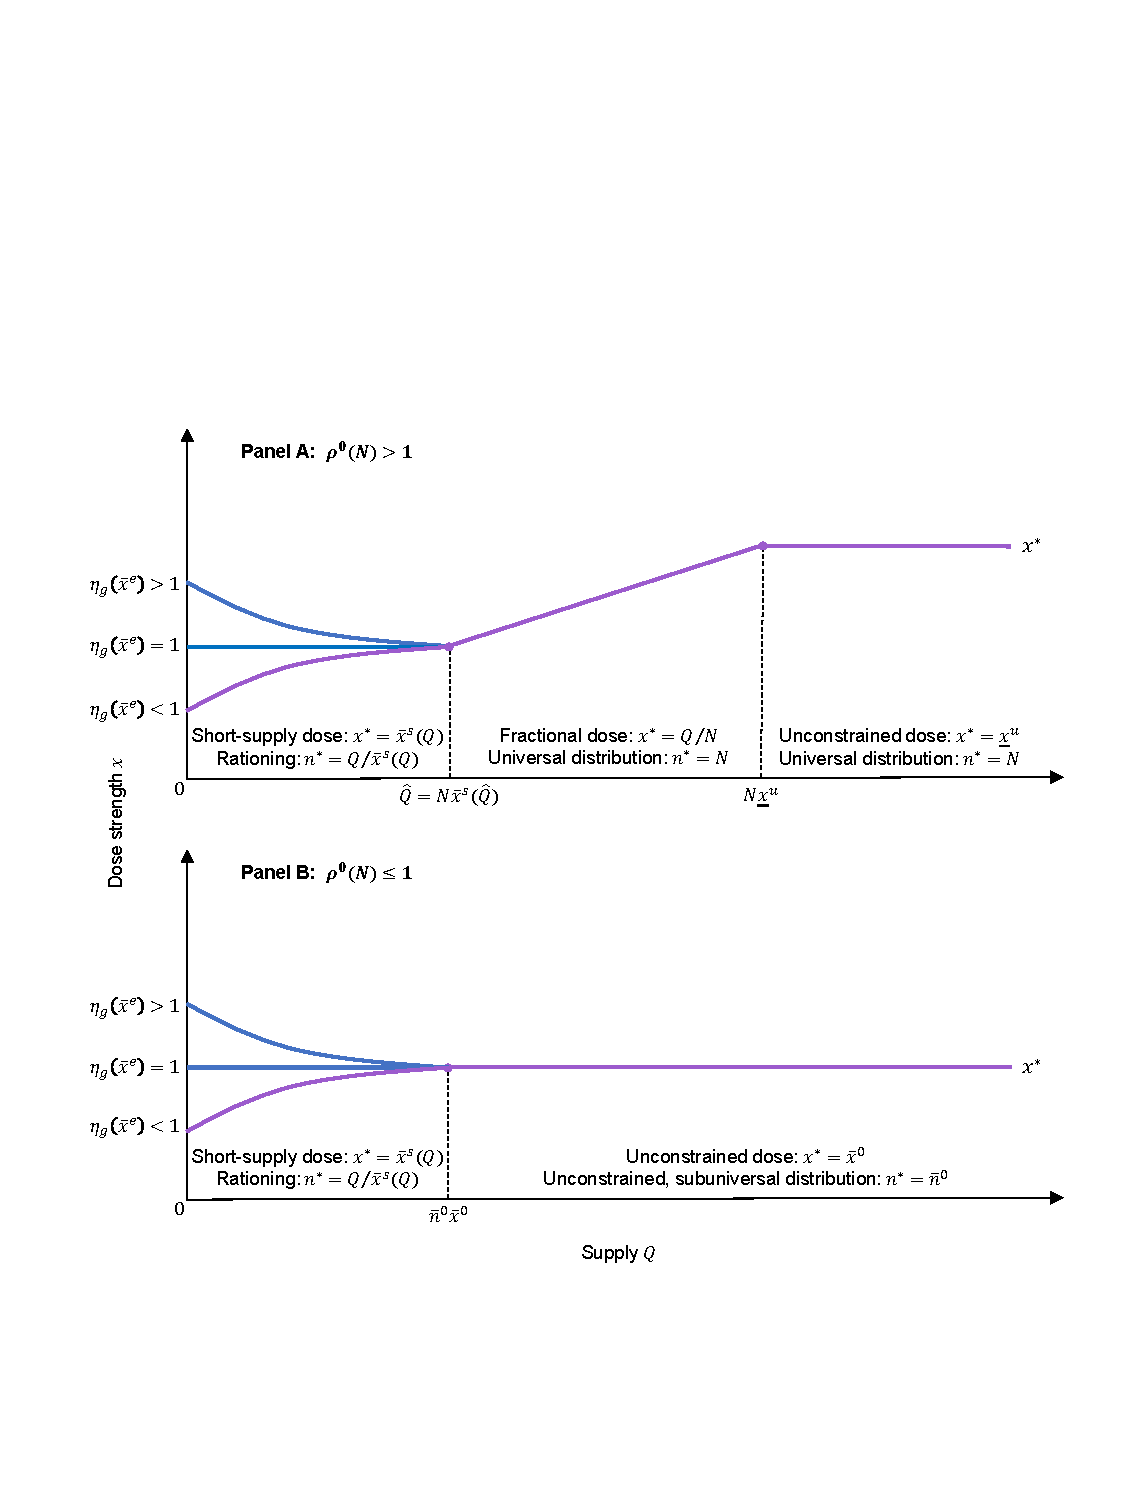
\includegraphics[viewport=40 110 530 515, width=.9\textwidth, clip]{figures/costly_optimum.pdf}
\vspace{1ex}
\caption{{\bf Optimal Dosage for Costly Vaccination.} The panels show
  the planner's optimal vaccine policy for various values of
  $\ratio(N)$. Unlike previous figures, here, panels distinguish
  between different parameter values, not different shapes for
  $\efficacy$. In the interval closest to the origin, the optimal dose
  corresponds to the short-supply dose $\xshortbar\!(Q)$, which may
  slope up, down, or be constant. The figure shows three example
  slopes, labeled with the necessary and sufficient condition from
  Proposition~\ref{p:xshort} for that slope. Purple curve segments (a
  blend of the colors used in previous figures) apply to both concave
  and strictly sigmoid $\efficacy$; blue segments apply only to
  strictly sigmoid $\efficacy$.}
\label{fig:costly_optimum}
\end{figure}

As $Q$ falls below $N \xunivlbar$, the capacity constraint begins to
bind. The optimal dose is initially stretched so all individuals can
still be vaccinated.  For sufficiently tight capacity, below threshold
$\Qhat$, the optimum switches to the short-supply dose,
$\xshortbar\!(Q)$. As we saw in Proposition~\ref{p:xshort}, the
comparative statics here are ambiguous: $\xshortbar\!(Q)$ may
increase, decrease, or remain constant as $Q$ falls, depending on
whether generalized cost is more or less elastic than efficacy at
$\xunitbar$. These comparative statics are inherited by the optimal
dosage $x^*$ since $x^* = \xshortbar\!(Q)$ in this region. It is
possible that $x^*$ increases as $Q$ falls. According to
Propositions~\ref{p:concave}--\ref{p:k}, the necessary and sufficient
conditions for this outcome are that $\efficacy$ is stricly sigmoid,
$\side$ is strictly convex, and $k$ is sufficiently low.

Extreme examples can be constructed in which the curve turns so
sharply upward as $Q$ approaches 0 that $\xshortbar\!(Q)$ is higher in
that limit than the unconstrained dose $\xunivlbar$. In such extreme
cases, $x^*$ is highest when supply constraints are the tightest.

The lower panel of Figure~\ref{fig:costly_optimum} illustrates the
case of a low benefit/cost ratio, $\ratio(N) \leq 1$. In this case,
for sufficiently high supply $Q$, unconstrained doses are distributed,
but to less than the entire population. It is optimal to leave some
individuals unvaccinated not because of scarce supplies but because
the marginal benefit of vaccinating them is less than the marginal
generalized cost. The optimal vaccine policy unconstrained by supplies
or population happens to involve an interior number of
vaccinations. As capacity is tightened and $Q$ falls below $\nnobar
\xnobar$, the supply constraint starts to bind, and the optimal policy
switches to short-supply dosing $\xshortbar\!(Q)$. Decreasing $Q$ in
this interval can increase, decrease, or leave the optimal dose
constant as in the upper panel of the figure.

%%%%%%%%%%%%%%%%%%%%%%%%%%%%%%%%%%%%%%%%%%%%%%%%%%%%%%%%%%%%%%%%%%%%%%%%%%%%%%%

\Section{Extensions}
\label{s:Extensions}

This section analyzes two extensions to the original model. First, we
consider an alternative efficacy function that has an interior peak
instead of being everywhere increasing. Second, we consider allow for
uncertainty in the level of efficacy at the time the planner sets the
dosage.

%------------------------------------------------------------------------------

\SubSection{Peaked Efficacy}
\label{ss:Peaked}

In the model analyzed thus far, we took efficacy to be an increasing
function over its whole domain. Marginal efficacy remained positive
for any finite dose, no matter how large. In this subsection, we
consider an alternative model of peaked efficacy. In this alternative
illustrated in Figure~\ref{fig:peaked}, $\efficacy$ increases up to a
peak, denoted $\xpeak$, and decreases for larger doses. 

\begin{figure}[tp]
\centering
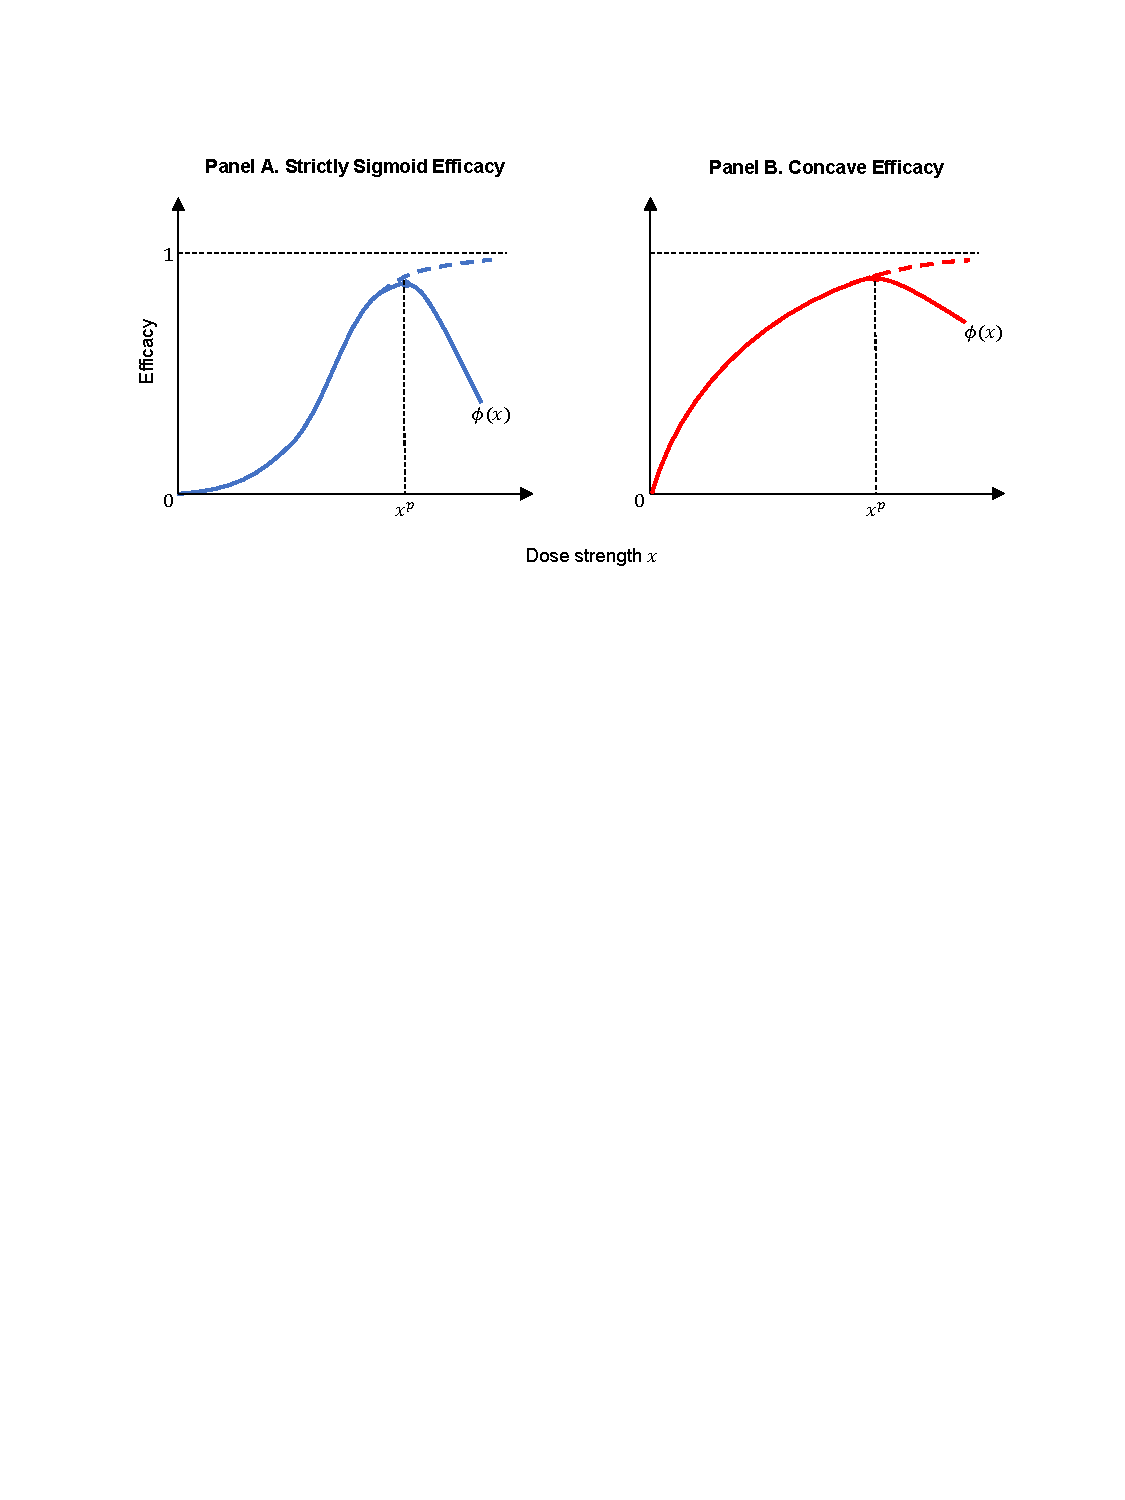
\includegraphics[viewport=65 445 495 645, width=.85\textwidth, clip]{figures/peaked.pdf}
\vspace{1ex}
\caption{{\bf Peaked Efficacy Function.} In the original model,
  $\efficacy$ continues to increase for the largest doses, illustrated
  by the dashed curves. The alternative model in this section involves
  peaked $\efficacy$, which turns down after reaching peak $\xpeak$,
  with reduced efficacy beyond that dosage.}
\label{fig:peaked}
\end{figure}

We have several motives for analyzing peaked efficacy. First, it is
consistent with some vaccinology studies. Experiments with animal
models found statistically significant evidence of a peak in the
dose-response functions
(\citealp{Pompano2014,Rhodes2016,Billeskov2018}; see meta-analysis in \citealp{Benest2020}). Second, we will adopt
peaked efficacy functions in our calibrations. As we will see, the
peak $\xpeak$ provides a well-defined notion of a full dose,
facilitating comparisions in the calibration section. Before turning
to the calibrations, it is useful to work out the implications of
peaked efficacy functions in the simpler model here first.

We model peaked efficacy by slightly modifying the specification of $\efficacy(x)$. We continue to assume $\efficacy$ is sigmoid for dosages smaller than $\xpeak$. For dosages larger than $\xpeak$, other than assuming $\efficacy(x) < \efficacy(\xpeak)$, we will be fairly agnostic about the properties of $\efficacy(x)$ since the optimum will not be found there. Formally, let peaked efficacy be the real-analytic function $\efficacy : [0, \infty) \rightarrow [0, 1]$ satisfying $\efficacy(0) = 0$, $\efficacy'(x) > 0$ for $x \in (0, \xpeak)$. We model the peak by assuming $\efficacy'(\xpeak) = 0$ and $\efficacy(x) < \efficacy(\xpeak)$ for all $x > \xpeak$. To ensure $\efficacy$ is sigmoid on $[0, \xpeak)$, we assume there exists $\xpoi \in [0,\xpeak)$ such that $\efficacy(x)$ is convex for all $x <\xpoi$ and $\efficacy(x)$ is concave for all $x \in (\xpoi, \xpeak]$.  

The following proposition characterizes the planner optimum
integrating peaked efficacy into the model with costless vaccination.
\begin{proposition}
\label{p:peaked_costless}
\singlespace
Suppose vaccination is costless to the planner, i.e., $\general(x) =
0$, and efficacy has a peak at $\xpeak$. The optimal policy vaccinates
$n^* = \min \{ Q/\xunitbar, N \}$ individuals with dose $x^* = \max
\bigl\{ \xunitbar, \min\{Q/N, \xpeak\} \bigr\}$.
\end{proposition}

\begin{figure}[tp]
\centering
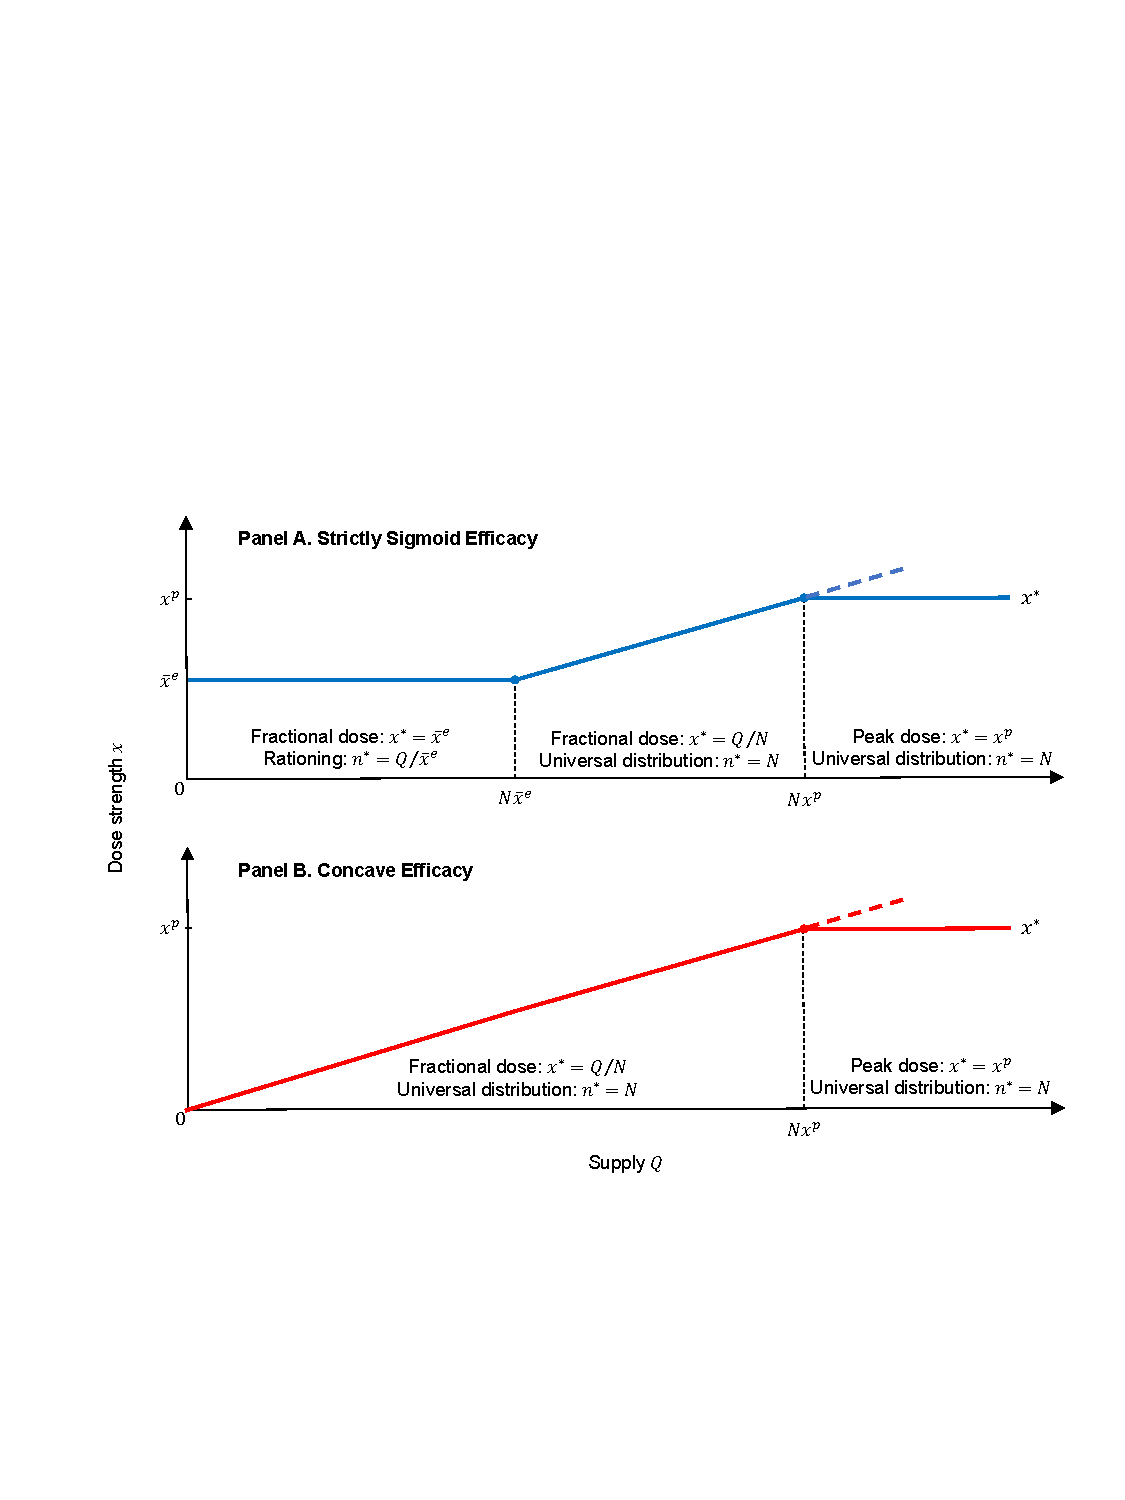
\includegraphics[viewport=50 155 530 475, width=.9\textwidth, clip]{figures/peaked_optimum.pdf}
\vspace{1ex}
\caption{{\bf Optimal Dosage with Costless Vaccination and Peaked
    Efficacy.} Moving from everywhere-increasing to peaked efficacy
  caps the planner optimum at $\xpeak$ but otherwise leaves it
  unchanged. The dashed line shows the optimum in the original model
  with everywhere-increasing efficacy for comparision.}
\label{fig:peaked_optimum}
\end{figure}

\noindent Figure~\ref{fig:peaked_optimum} helps visualize how the
planner optimum under costless vaccination changes with peaked
efficacy. The optimum is the same as in the original model except for
the imposition of a cap $\xpeak$ on the optimal dose. The planner has
no reason to go beyond $\xpeak$ since this only reduces social surplus
by reducing efficacy.

As straightforward as it was to integrate peaked efficacy into the
model with costless vaccination, integrating it into the model with
costly vaccination is even more so. The positive marginal generalized
cost of larger doses already provided a reason for the planner to
endogenously cap the dose below where efficacy flattens out. Thus, the
optimum prescribed in Proposition~\ref{p:costly} never ventures into
dosages where efficacy peaks and turns down. The optimal policy is the
same whether efficacy is everywhere-increasing or peaked, as the next
proposition states.
\begin{proposition}
\label{p:peaked_costly}
\singlespace
Suppose vaccination is costly to the planner, i.e., $\general(x) >
0$, and efficacy has a peak at $\xpeak$. The optimal policy remains
unchanged from Proposition~\ref{p:costly}. \end{proposition}

%------------------------------------------------------------------------------

\SubSection{Uncertain Efficacy}
\label{ss:Uncertain}

In this subsection, we extend the model to allow for residual
uncertainty in the efficacy function when the optimal dosage is
set. This formulation of the model captures the reality that
manufacturers seldom run late-stage clinical trials for more than one
dosage. Experimentation on dosage, if done at all, is restricted to
low-powered, early-stage trials and tends to be limited, only
investigating a handful of alternative doses. This was especially true
in the rush to develop \covid\ vaccines \citep{Dunn2023}.

Respecify the efficacy function as $\efficacy(x,\theta)$, adding a
second argument $\theta$ representing the unknown state of the world
when dosage $x$ is set. Assume high values of $\theta$ represent
``good news'' about efficacy and marginal efficacy: letting subscripts
denote partial derivatives with respect to those arguments, we have
$\efficacy_\theta > 0$ and $\efficacy_{x\theta} > 0$. Once $x$ is set,
assume it is difficult to change, perhaps requiring new clinical
trials or adjustments to manufacturing processes. Ex post, clinical
trials and medical experience with chosen dosage $x$ may reveal
information about $\theta$ that is not available ex ante, when $x$ is
set. Assume $\theta$ is randomly distributed on support $[0, \infty)$
  with probability density function $f(\theta)$ and cumulative
  distribution function $F(\theta)$.

With the addition of uncertainty complicating the analysis, we seek to
streamline the analysis by considering the simplest variant of the
model along other dimensions. In particular, throughout this
subsection, we will maintain the assumptions that efficacy is concave
in $x$, i.e., $\efficacy_{xx} < 0$, and that vaccination is costless,
i.e., $\general(x) = 0$. Under these assumptions, were efficacy not
peaked, the optimal dosage would simply be $x^* = Q/N$ with or without
uncertainty over $\theta$. Uncertainty would play no role in the
analysis.

Uncertainty does play a role when efficacy is peaked, motivating us to
adopt this the variant of the model throughout this
subsection. Intuitively, the optimal dose set under ex ante
uncertainty $x^*$ may turn out to be too strong in the light of
further information about $\theta$. If it is possible to adjust $x^*$
ex post, moving to a fractional dose could increase efficacy. Thus,
uncertainty provides another rationale for fractional dosing apart
from epidemic supply constraints.

To integrate uncertainty and peaked efficacy in the same model, assume
for all $\theta \in (0, \infty)$, there exists $\xpeak(\theta) > 0$
such that $\efficacy_{x} \bigl( \xpeak(\theta), \theta \bigr) =
0$. Totally differentiating with respect to $\theta$ and rearranging
yields
\begin{equation}
\label{dxpeak}
\frac{d \xpeak(\theta)}{d \theta} = - \frac{\efficacy_{x\theta} \bigl(
  \xpeak(\theta), \theta \bigr)}{\efficacy_{xx} \bigl( \xpeak(\theta),
  \theta \bigr)} > 0.
\end{equation}
Since $\efficacy_{xx} < 0$, we have $\efficacy_{x}( x, \theta) > 0$
for all $x \in \bigl[ 0, \xpeak(\theta) \bigr)$ and $\efficacy_{x}( x,
  \theta) < 0$ for all $x > \xpeak(\theta)$.
 
To highlight the possibility that uncertainty can provide a rationale
for fractional dosing apart from supply constraints, we will abstract
from any constraint on $Q$ in this analysis. In the absence of a
constraint on supply, since vaccination is costless and more
vaccinations produce a positive benefit---i.e., $\benefit'(v) > 0$ for
all $v \geq 0$---it is immediate that the planner's optimum involves
vaccinating as many individuals as possible: $n^* = N$. The optimal ex
ante dose $x^*$ maximizes the expected social benefit of the universal
vaccine campaign,
\begin{equation}
\label{max_uncertainty}
\max_{x \geq 0} \left[ \int_0^\infty \benefit \! \bigl( N \efficacy(x,
  \theta) \bigr) f(\theta) d\theta \right],
\end{equation}
satisfying the first-order condition
\begin{equation}
\label{foc_uncertainty}
\int_0^\infty \benefit' \! \bigl( N \efficacy(x^*, \theta) \bigr)
\efficacy_x (x^*, \theta) f(\theta) d\theta = 0.
\end{equation}
Since $\benefit' > 0$ and $f > 0$, the left-hand side of
\eqref{foc_uncertainty} can only equal 0 if it integrates some
positive and negative values of $\efficacy_x$. Moreover, since
$\efficacy_{x\theta} > 0$, equation \eqref{foc_uncertainty} implies
the existence of $\hat{\theta}(x^*) > 0$ such that $\efficacy_x \bigl(
x^*, \hat{\theta}(x^*) \bigr) = 0$, $\efficacy_x (x^*, \theta) < 0$
for all $\theta \in \bigl( 0, \hat{\theta}(x^*) \bigr)$, and
$\efficacy_x (x^*, \theta) > 0$ for all $\theta > \hat{\theta}(x^*)$.

Focusing on those states of the world $\theta$ below
$\hat{\theta}(x^*)$, we have that the ex ante optimal dose turns out
to be beyond the efficacy peak in those states: formally, $x^* >
\xpeak(\theta)$. If the true state $\theta$ were learned and it was
possible to reduce dosage ex post, a fractional dose would improve
social welfare in those states. The probability that the ex ante
optimal dose turns out overly strong equals $F \bigl(
\hat{\theta}(x^*) \bigr)$. If the efficacy peak were known, it would
be optimal to set $x^*$ to that peak. Given the peak is uncertain when
$x^*$ is set in the model, the optimal value under uncertainty
balances undershooting the peak versus overshooting, and thus
optimally entails a positive probability of overshooting. It may not
be possible to adjust $x^*$, but if it is, there is a positive
probability $F \bigl( \hat{\theta}(x^*) \bigr)$ that moving to a
fractional dose improves efficacy. This finding is just a consequence
of uncertainty, independent of supply constraints that provide
additional rationale for fractional dosing.

%%%%%%%%%%%%%%%%%%%%%%%%%%%%%%%%%%%%%%%%%%%%%%%%%%%%%%%%%%%%%%%%%%%%%%%%%%%%%%%

\Section{Calibrations of Epidemiological Model}
\label{s:Calibrations}

This section moves from a static, reduced-form model to a detailed
epidemiological model. The analysis of the simpler model had the
advantage of producing analytical results that hold generally rather
than just for calibrated parameters. The analysis in this section has
a number of offsetting advantages.

The model incorporates dynamics in both the spread of the disease and
the distribution of vaccine to the population. The dynamics are not
merely a better approximation of reality; they bring forth
new economic insights. In the static model, it was possible to install
enough capacity $Q$ to relieve the constraint on vaccine supplies. In
a dynamic model, the constraint always binds. Whatever the installed
capacity $Q$, were it doubled, the time to complete the vaccination
campaign would be cut in half.  The richer model also incorporates
heterogeneity in mortality risk and contact rates across age
cohorts. Beyond improving the model's realism, this addition opens up
the possiblity of a new policy to investigate, moving from uniform to
age-specific doses.

We calibrate the model with parameters drawn from the
\covid\ pandemic. The analysis thus far has suggested the theoretical
possibility that fractional improves on full dosing. Here, we are
interested in learning whether the theoretical possibility is relevant
for realistic parameters and, if so, how small optimal fractional
doses are and how much surplus is gained from that policy.

While most parameters are calibrated to the \covid\ pandemic, we leave
some free for comparative-statics analysis. The main one is the
constraint on vaccine supply. We consider possibilities ranging from a
small fraction to several multiples of the supply available during the
\covid\ pandemic. We seek to determine how optimal fractional dosing
varies with the tightness of supply. We also consider both concave and
sigmoid shapes for the efficacy function. To determine which was
relevant for \covid\ vaccines would require data from the low end of
the dose-response curve, which is mostly lacking for
\covid\ vaccines. In place of a known functional form, we explore the
sensitivity of the results to various alternatives. In addition, given
the considerable space allocated to separately analyzing each
functional form, we are interested in seeing whether the functional
forms lead to any practical difference in policy calibrations.

%------------------------------------------------------------------------------

\SubSection{SEIRDV Model}

To account for the dynamics of infection, mortality, and vaccination,
we adopt a compartmental epidemiological model, the workhorse of
mathematical epidemiology \citep{Anderson1992}. In particular, we
adopt an extension of the classic and commonly used
susceptible-exposed-infected-recovered model that includes vaccination
and mortality dynamics, abbreviated SEIRDV.  The model used here is a
slight modification of the one described in detail in in own prior
work \citep{Wiecek2022}. Here, we give only a short exposition.

The population is stratified into age cohorts indexed by $a = 1,
\ldots, A$. Each age cohort is further subdivided into the
compartments shown in the schematic diagram in
Figure~\ref{fig:seird}. Susceptible individuals ($S_a$) who come into
contact with someone who is infectious may be exposed to the disease
($E_a$) and themselves become infected ($I_a$). Some infected
individuals die ($D_a$); the others recover ($R_a$), obtaining natural
immunity. Susceptible individuals may be vaccinated. If the
imperfectly effective vaccine happens to work, the individual is
protected from infection ($P_a$); otherwise they are without protection ($W_a$).

\begin{figure}[tp]
\centering
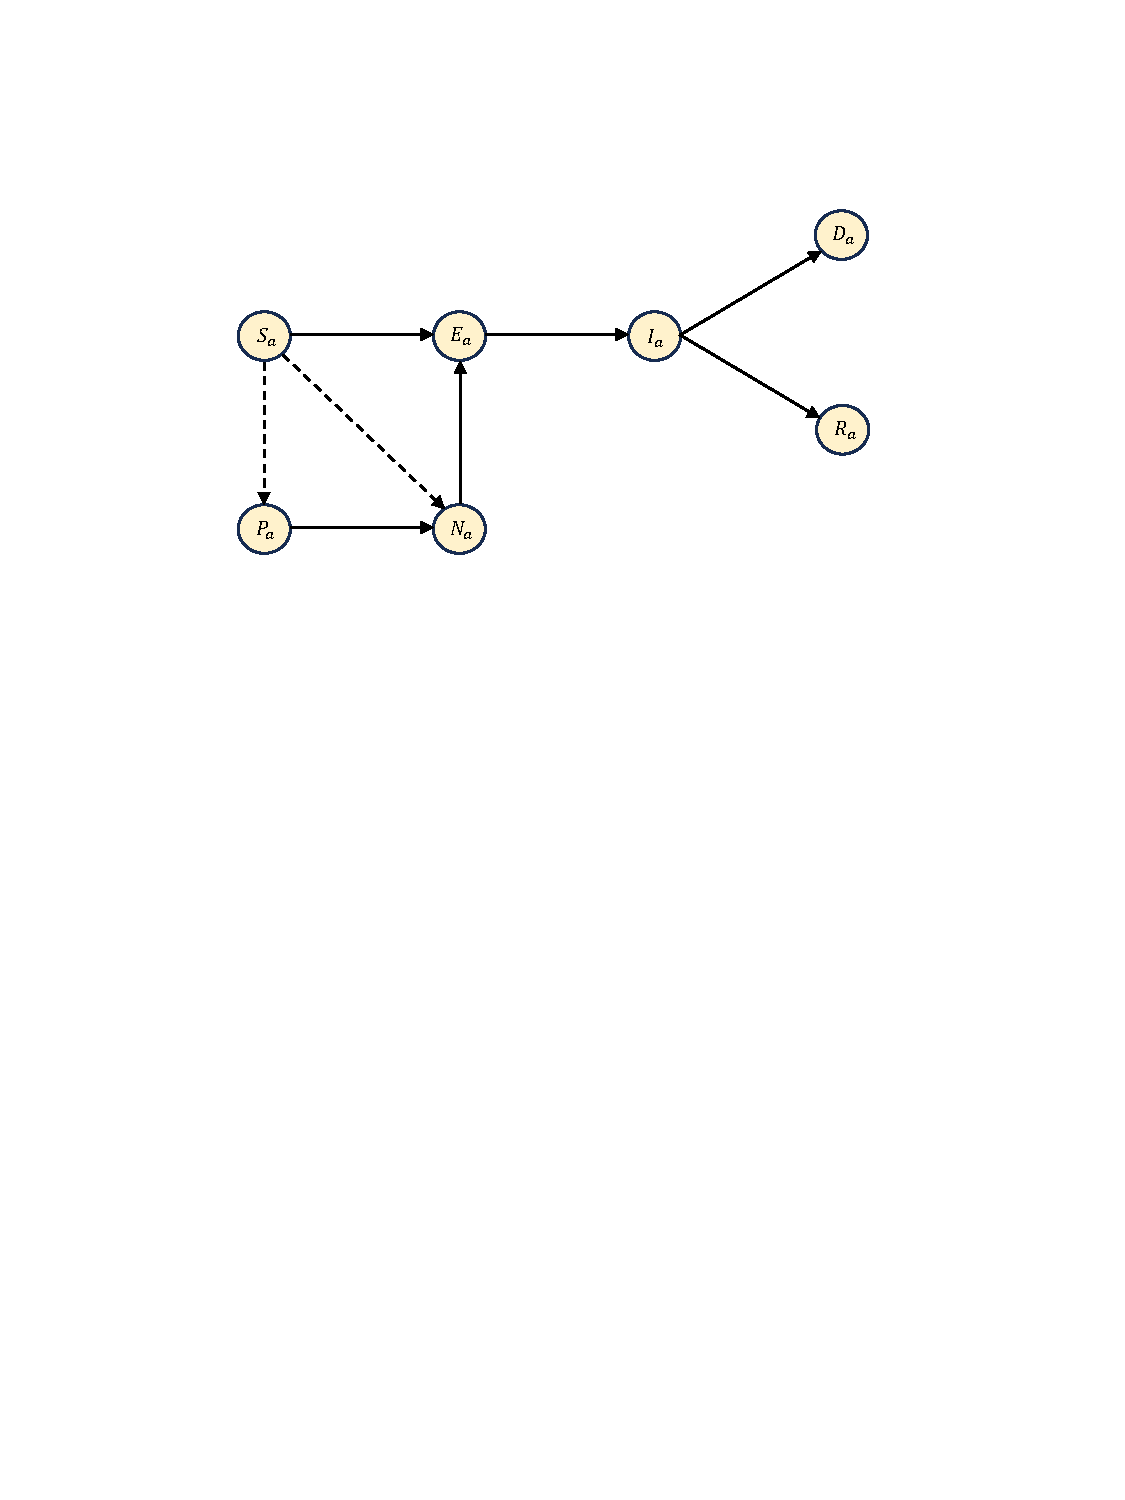
\includegraphics[viewport=110 450 465 625, width=.7\textwidth, clip]{figures/epi_model.pdf}
\caption{{\bf Schematic Diagram of SEIRDV Model.} Arrows indicate
  flows between compartments. Dashed arrows represent
  vaccinations. The model allows for heterogeneity by age cohort, as
  indicated by the $a$ subscripts.}
\label{fig:seird}
\end{figure}

More formally, members of each age cohort move between compartments
according to the following differential equations:
\begin{align}
\dot{S}_a(t) &= - \lambda_a(t) S_a(t) - q_a(t) \label{S} \\
\dot{E}_a(t) &= \lambda_a(t) [ S_a(t) + W_a(t) ] - \epsilon_a E_a(t) \label{E} \\
\dot{I}_a(t) &= \epsilon_a E_a(t) - \xi_a I_a(t) \label{I} \\
\dot{R}_a(t) &= (1 - \mu_a) \xi_a I_a(t) \label{R} \\
\dot{D}_a(t) &= \mu_a \xi_a I_a(t) \label{D} \\
\dot{P}_a(t) &= q_a(t) \efficacy(x_a) \label{P} \\
\dot{W}_a(t) &= q_a(t) [ 1 - \efficacy(x_a)] - \lambda_a(t) W_a(t). \label{W} 
\end{align}
Susceptible individuals, in compartment $S_a(t)$, become infected at
rate $\lambda_a(t)$, which depends on contacts with infectious
individuals in various cohorts:
\begin{equation}
\label{contact}
\lambda_a(t) = \beta \sum_{a' = 1}^A c_{a, a'} I_{a'}(t).
\end{equation}
Parameter $\beta$ captures the virus' transmissibility; $c_{a, a'}$ is
an element of the contact matrix, equal to the number of contacts made
by an individual in cohort $a$ with members of cohort $a'$.

Upon infection, individuals move from the susceptible to the exposed
compartment $E_a$, where they remain while the virus incubates, moving
to the infectious compartment $I_a$ at a rate $\epsilon_a$ determined
by the virus' incubation period. Individuals in the infectious
compartment are able to transmit the virus to others. Individuals exit
the infectious compartment at rate $\xi_a$ determined by the virus'
infection period. They then either die---entering compartment $D_a$
with probability $\mu_a$ determined by the age-specific infection
fatality rates---or recover---entering compartment $R_a$ with
probability $1 - \mu_a$. Recovered individuals obtain natural
immunity, which for most of the analysis we assume does not
wane.\footnote{Assuming natural immunity does not wane is a reasonable
approximation given the calibration traces a single epidemic outbreak
over an interval of months, not years.}

Each unit of time, $q_a(t)$ susceptibles in cohort $a$ are vaccinated, given by
\begin{equation}
\label{qat}
q_a(t) = v_a(t) \left( \frac{Q}{x_a} \right) \left[ \frac{S_a(t)}{S_a(t) + R_a(t)} \right].
\end{equation}
The first factor, $v_a(t)$, captures the vaccine prioritization strategy; $v_a(t)$ is an indicator function
that turns on when the cohort is eligible to receive the vaccine and
remains on until the campaign is completed for that cohort. While the cohort is being vaccinated, all available supply $Q$ is dedicated to it. Measuring $Q$ in full-dose equivalents and taking $x_a$ to be the fraction of a full dose received by cohort $a$, we have that the supply of fractional doses to the cohort while it is vaccinated equals the second factor, $Q/x_a$. This factor implies that moving to a smaller fractional dose allows the supply rate to increase. The last, bracketed factor reflects a modeled information friction---that recovered and susceptible individuals cannot be distinguished, so
both compartments end up being vaccinated. Since recovered individuals
already have natural immunity, the vaccine is effectively wasted on
them.\footnote{For simplicity, we do not distinguish between vaccinated and unvaccinated individuals in the recovered compartment, $R_a$. Those arriving in $R_a$ because their initial vaccination was ineffective can end up being vaccinated multiple times. Repeat vaccinations have no benefit in the model because recovered individuals are not later infected. A more complex policy that attempts to reduce ``leakage'' to the $R_a$ compartment by prohibiting repeat vaccinations has a negligible effect on outcomes.} The bracketed factor is the share of cohort $a$ vaccinations received by the susceptible individuals who can benefit from it. 

As in the
reduced-form model, we assume that the vaccine is all-or-nothing,
providing perfect protection (perfectly preventing transmission,
disease, and death) for an individual with a probability given by the
vaccine's efficacy, $\efficacy(x_a)$, moving them to compartment
$P_a$. We abstract from the time required to develop immunity
following vaccination. With probability $1 - \efficacy(x_a)$, the
vaccine does not work for the person, so they are without protection,
moving to compartment $W_a$. Individuals are assumed to retain any immunity conferred by vaccination or induced by contracting the disease for the remainder of the epidemic, implying there is no exit from compartments $P_a(t)$ or $R_a(t)$. Individuals in $W_a$, who are without protection, exit that compartment when they are infected,
which occurs at the same rate $\lambda_a(t)$ as for susceptible
individuals.

Possible imperfections in the vaccine campaign are captured via three
model assumptions. First, the vaccine is
imperfectly effective, i.e., $\efficacy(x_a)< 1$. Second, the bracketed factor in equation \eqref{qat} is the proportion received by susceptible consumers in the cohort. The rest is given to the recovered compartment; the vaccine is effectively wasted on them since they already have  natural immunity. Third, we assume
that loss of vaccine-induced immunity is unobservable, so the move
from $P_a$ to $W_a$ cannot be prevented by revaccinating the
individual.

%------------------------------------------------------------------------------

\SubSection{Calibration Parameters and Methods}

We calibrate model parameters to the outcomes of initial clinical
trials of the first effective \covid\ vaccines and mass vaccination
campaigns that began in late 2020 and continued through 2021, when all
countries faced shortage of vaccines. Appendix~\ref{A:Inputs} collects the calibration parameters and
initial compartment values in a series of tables.

Our goal is to guide the
selection of roughly plausible parameters. Providing an accurate
portrayal of the \covid\ pandemic is beyond the scope of this exercise
for several reasons. First, outcomes varied widely across countries;
in taking the global average for a parameter, we may fail to reflect
the experience in any given region. Second, the all-or-nothing nature
of the vaccine in the model allows for a single notion of the efficacy
of the vaccine, which works equally well to prevent infection,
disease, severe disease, or death. In reality, \covid\ vaccines were
more effective at preventing deaths and hospitalizations than
preventing transmission, and this distinction only grew with emergence
of variants, which we do not model. Most importantly, our
specification of the SEIRDV model has a single epidemic outbreak. This
may not be unrealistic if interpreted as applying to the first wave
caused by the ancestral strain of \covid\ but becomes increasingly
unrealistic with the emergence of \covid\ variants, leading to
infection cycles, which the model is not designed to
capture.\footnote{\citet{Wiecek2023} analyzes a model allowing for
infection cycling, finding that estimates of vaccine benefits are
sensitive to fine model details concerning the partial immunity
afforded by the primary vaccine series against future variants, the
timing of boosters, and so forth.}

\paragraph{Age Cohorts.}

We partition the population into nine age cohorts: two cohorts of
children aged 0--9 and 10--19 and seven cohorts of adults, aged 20--29, 30--39,
40--49, 50--59, 60--69, 70--79, and 80 and above.

\paragraph{Virus Transmission.}

We calibrate the contact matrix $(c_{a,a'})$ to the frequency of
interactions between different age groups from the large-scale surveys
of European countries in \citet{Mossong2008}.  The basic reproductive
number, $\Rzero$, represents the average number of new infections
generated by a single infected individual in a fully susceptible
population. We calibrate the transmissibility parameter $\beta$ so
that the model delivers a value of $\Rzero = 2$. This round value of
$\Rzero$ is not meant to be a precise estimate\footnote{In reality,
$\Rzero$ did not have a single, well-defined value for \covid\ but
varied widely across regions and time in response to social
distancing, lockdowns, and continual emergence of new variants of the
virus.} but illustrative of a relatively fast-moving epidemic like
\covid. The appendix provides a calibration for a slower growing
epidemic, with $\Rzero = 1.1$.

\paragraph{Fatality Rate.}

We calibrate the infection fatality rate $\mu_a$ using estimates from
\citet{Verity2020}, ranging from 0.03\% for the youngest adult cohort
(20--29 year-olds) up to 9.3\% for the oldest cohort (80 and
above).\footnote{The \citet{Verity2020} estimates are based on
large-scale surveys in Europe of mortality from ancestral
\covid. While \covid\ mortality rates varied across countries and over
time, particularly as new variants emerged, the log-linear increase of
mortality with age found in \citet{Verity2020} is consistent across
studies.} These calibrated values of $\mu_a$ entail that the
population mortality rate is 0.55\% in the absence of vaccination in
the model; roughly 1\% of infected individuals die.

\paragraph{Vaccine Supply.}

Turn now to calibrating the vaccine side of the model, starting with
vaccine supply. For ease of interpretation, we express supply relative to population size, $Q/N$, measuring the percentage of the population that can be vaccinated with full doses per day. We allow vaccine supply to range over several orders of magnitude
(0.01\%, 0.1\%, 1\%, and 10\%), spanning possibilities from negligible
to virtually unconstrained supplies. For example, a daily 0.1\% supply
achieves 50\% coverage of the population with full doses in just over
16 months. We take 0.1\% as the benchmark supply, since the associated
time to achieve 50\% coverage is close to the median 14 months across
countries during the \covid\ pandemic.\footnote{We calculated this
figure using data from \citet{OWID_COVID_Vax}, taking the start of the
vaccination period as December 2, 2020, the first date vaccines were
distributed in any country. Supplies varied dramatically across
countries. Gibralter was the fastest country to 50\% coverage with
full doses, which it achieved in about three months; the United States
and median European Union country took about eight months; 38\% of
countries never achieved that coverage.}

\paragraph{Vaccine Prioritization.}

To calibrate the vaccine prioritization embodied in $v_a(t)$, note
that, while the details varied from country to country, most followed
the general principle that individuals at greatest risk of severe
disease or death should be vaccinated first. Advanced age was
typically a leading factor in the prioritization
\citep{WHO2020,Williams2021}. Since our model only considers
heterogeneity in age and not other characteristics like comorbidities
or healthcare work, we specify a strict age-based prioritization,
where each cohort is vaccinated in descending age order. The cohort
whose turn it is to receive the vaccine receives the entire
available supply until the ceiling on cohort members who can be reached are vaccinated. We assume
80\% of each cohort can be reached and 20\% not (perhaps
due to logistical frictions or vaccine hesitancy).\footnote{Overall,
80\% was the upper limit of vaccination coverage at the end of the
pandemic (by 2023 United States reached 69\% fully vaccinated, Germany
76\%, United Kingdom 75\%). In 2021 it was typical for countries with
good supply to reach over 80\% in highest risk groups and much lower
in general population. This pattern differed considerably across
countries (by 2023 Nigeria reached 30\%, Ethiopia 35\%, Democratic
Republic of Congo below 10\%; all figures according to
\citet{OWID_COVID_Vax}).} We conduct a sensitivity analysis where we reduce the ceiling on cohort members who can be reached to 60\%. We assume that the cohorts of children
cannot be vaccinated, echoing the fact that \covid\ vaccines were not
initially approved for children.

\paragraph{Dose-Response.}

Our calibrated dose-response curves are shown in
Figure~\ref{fig:dose_response}. We started with flexible sigmoid and
concave functions, having three free parameters each. For each curve,
we solve for the value of the three parameters that allow the curve to
fit the three data points observed for \covid\ vaccines, labeled $A$,
$B$, and $C$ in the figure. Details behind the specific functional
forms used and parameters obtained are provided in the appendix.

Point $A$ corresponds to the full doses of approved vaccines used
during the pandemic. We normalize the dose strength at point $A$ to to
$x = 1$ and set the efficacy to $\efficacy(1) = 0.95$, approximating
the efficacy of the mRNA vaccines against symptomatic infection in
early clinical trials \citep{Baden2020,Polak2020}. Point $B$
corresponds to a half-strength dose. Evidence summarized in
\citet{Wiecek2022} puts a reasonable estimate of the efficacy of a
half dose at $\phi(0.5) = 0.8$. Point $C = (0,0)$ embodies the
assumption that a dose with no active ingredient is useless.

\begin{figure}[t]
\centering
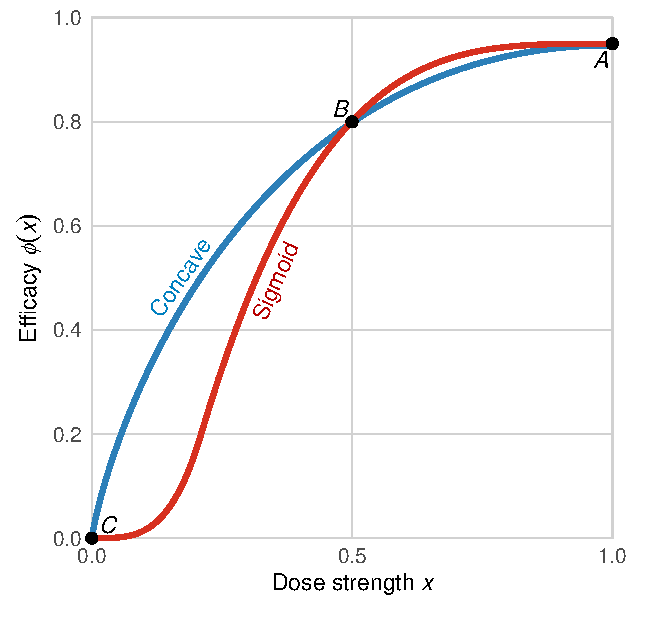
\includegraphics[width=.55\textwidth, clip]{figures/dose_response_edited.pdf}\\[-1ex]
\caption{{\bf Calibrated Dose-Response Functions.} The general
  functional forms for the curves are provided in equations
  \eqref{a:calibration_concave} and \eqref{a:calibration_sigmoid} in
  the appendix. Curves are calibrated to pass through points $A$, $B$,
  and $C$ and satisfy derivative condition $\phi'(1) = 0$, ensuring
  $A$ is the peak of the efficacy function, thus representing a full
  dose.}
\label{fig:dose_response}
\end{figure}

The specifications we chose for the efficacy functions happen to pass
through point $C$ for all parameters, so an additional condition is
required to pin down the three parameters.  The additional condition
is derived from the assumption that efficacy peaks at $A$ and there is
no marginal efficacy beyond that dosage. Formally, $\xpeak = 1$,
implying $\phi'(1) = \phi'(\xpeak) = 0$.  Assuming efficacy peaks at
$A$ preserves the internal consistency of the calibration. Given that
we will abstract from the generalized cost of vaccination, setting
$g(x) = 0$, the only reason for limiting the strength of full doses is
because efficacy peaks there.

\paragraph{Generalized Costs.}

The calibration abstracts from planner expenditures on vaccines and
side effects, setting generalized costs, $g(x)$, to zero. We have
practical and pedagogical grounds for this abstraction. On practical
grounds, setting $g(x) = 0$ is a reasonable approximation, since
serious side effects from \covid\ vaccines were shown to be very rare
\citep{Faksova2024GVDN} and social benefits were estimated to be two
orders of magnitude greater than the price countries paid for the
vaccine \citep{Castillo2021}. On pedagogical grounds, setting $g(x) =
0$ absolves us from having to monetize mortality and morbidity losses
to weigh against expenditures.

\paragraph{Calibration Methods.}

While some simple compartmental models admit analytic solutions
\citep[see, e.g.,][]{Goodkin-Gold2024}, complex models like the one
here---with more compartments and heterogeneous cohorts---have no
known analytic solutions. Therefore, we rely on numerical methods to
simulate the time path of the model's compartments and evaluate the
objective function behind the dose-optimization problem.\footnote{We
use the \pkg{odin} package in R to solve the differential-equation
system and the \pkg{nloptr} package in R (with tolerance set to
\num{1e-06}) for dose optimization. All of our code is available at
\url{https://github.com/DevInnovationLab/optimal_dose}.} We run all
simulations for 360 days.

\paragraph{Epidemic Diagram.}

Figure~\ref{fig:example_model} shows the evolution of compartments in
the model for various levels of capacity to vaccinate a flow of the
population with full doses. At the calibrated value of the basic
reproductive number, $\Rzero = 2$, the epidemic grows relatively
fast. In the absence of vaccines, infections peak at about four months
and about 55\% of population are eventually infected.

\begin{figure}[tp]
\centering
\includegraphics{figures/example_model_edited.pdf}\\[-3ex]
\caption{{\bf Evolution of Compartments in Calibrated Model.}
  Simulates outcome from SEIRDV model for various levels of vaccine
  capacity. Assumes vaccines are full doses and dose response is concave. Simulation allows proportions in compartments to vary
  across age cohorts; graphs here aggregate age cohorts, showing
  proportions of total population.}
\label{fig:example_model}
\end{figure}

%------------------------------------------------------------------------------

\SubSection{Calibration Results}

This subsection presents the results for the planner's optimal dosing
policy in the calibrated model. Given that we have abstracted from
generalized costs of vaccines, $g(x)$, the planner's objective reduces
to choosing dose strength to maximize health benefits, or
equivalently, to minimize epidemic harms. We will simplify further by
abstracting from morbidity losses and consider only mortality
losses. We also abstract from discounting and years of lost life,
measuring mortality losses simply by the total number of deaths.

We solve for two versions of the optimal fractional-dosing policy, an
age-invariant (uniform) fractional dose and age-varying fractional
doses. The uniform fractional-dosing policy involves optimizing over a
single variable $x \in [0,1]$. The age-varying fractional-dosing
problem involves optimizing over a seven-dimensional vector of dose
strengths $(x_a)$.

The performance of these fractional-dosing policies will be gauged
against a no-vaccine benchmark and a full-dose benchmark. Formally,
let $\alldeaths = \sum_{a=1}^A D_a(T)$ denote aggregate deaths caused
by the epidemic by the end of the calibration summed across age
cohorts. Adding an argument $\alldeaths(X)$ allows us to distinguish
deaths under various vaccine policies $X$. Thus, $\alldeaths(0)$
denotes aggregate deaths under no vaccine, $\alldeaths(\xpeak)$ under
full doses, $\alldeaths(x^*)$ under optimal uniform fractional dosing,
and $\alldeaths(x_a^*)$ under optimal age-varying fractional
dosing. The performance of policy $X$ will be measured in two ways: reduction in deaths relative to a no-vaccine benchmark,
\begin{equation} 
\label{performance_no_vaccine}
\frac{\alldeaths(0) - \alldeaths(X)}{\alldeaths(0)},
\end{equation}
and relative to a full-dose benchmark,
\begin{equation}
\label{performance_full_dose}
\frac{\alldeaths(\xpeak) - \alldeaths(X)}{\alldeaths(\xpeak)}.
\end{equation} 

Table~\ref{tab:results} presents the results for various levels of
vaccine capacity and for both shapes of the dose-response
function. Focus first on the results for the benchmark supply (0.1\%
of the population vaccinated each day) and sigmoid dose-response
function. In that case, full doses avert 32\% of the deaths under no
vaccination. To stretch such a modest capacity, the optimal uniform
dose ends up being about half of a full dose. Distributing these
smaller doses more quickly allows the planner to avert 44\% of
deaths. With ten times more vaccine supply than the benchmark (1\% of
the population vaccinated each day), full doses avert most deaths
(88\%). Capacity of this magnitude speeds doses to the population so
quickly that there is little gain from speeding the process further
with fractional doses. Uniform fractional doses are 70\% of the
strength of full doses, averting 91\% of deaths, only three percentage
points more than full doses.  When vaccine supply is increased another
ten fold---to 10\% of the population vaccinated each day---at that
point supply is all but unconstrained, essentially leaving no room for
fractional doses to generate improvements. Full doses already avert
nearly all deaths (95\%). 

\begin{table}[t]
\caption{{\bf Calibration Results for Optimal Dosing and Averted Deaths}}
\label{tab:results}
\footnotesize
\begin{tabularx}{\textwidth}{@{} l *6{Y} @{}}
\toprule
& \mc{3}{c}{Fraction of full dose} & \mc{3}{c}{Fraction of no-vaccine deaths averted} \\ 
& \mc{3}{c}{$X / \xpeak$} & \mc{3}{c}{$[\alldeaths(0) - \alldeaths(X)] / \alldeaths(0)$} \\ \cmidrule(lr){2-4} \cmidrule(l){5-7}
 & & & Age-& & & Age-\\
Vaccine capacity  & & Uniform & varying & & Uniform & varying \\
(fraction of & Full & fractional & fractional & Full & fractional & fractional \\
population & dose & dose & dose & dose & dose & dose \\
supplied per day) & $X = \xpeak$ & $X = x^*$ & $X = (x_a^*)$ & $X = \xpeak$ & $X = x^*$ & $X = (x_a^*)$ \\ 
\midrule	
\mc{7}{c}{\bf Sigmoid Dose Response} \\[2ex]
0.01\% & 100\% & 42\% & \mc{1}{c}{Fig.~\ref{fig:age_solutions_both}} & 4\% & 7\% & 7\% \\
0.1\% & 100\% & 51\% & \mc{1}{c}{Fig.~\ref{fig:age_solutions_both}} & 32\% & 44\% & 44\% \\
1\% & 100\% & 70\% & \mc{1}{c}{Fig.~\ref{fig:age_solutions_both}} & 88\% & 91\% & 91\% \\
10\% & 100\% & 91\% & \mc{1}{c}{Fig.~\ref{fig:age_solutions_both}} & 95\% & 95\% & 95\% \\
\midrule
\mc{7}{c}{\bf Concave Dose Response} \\[2ex]
0.01\% & 100\% & 7\%  & \mc{1}{c}{Fig.~\ref{fig:age_solutions_both}} & 4\%  & 11\%  & 11\% \\
0.1\% & 100\% & 35\% & \mc{1}{c}{Fig.~\ref{fig:age_solutions_both}} & 32\% & 45\% & 46\% \\
1\% & 100\% & 73\% & \mc{1}{c}{Fig.~\ref{fig:age_solutions_both}} & 88\% & 90\% & 90\% \\
10\% & 100\% & 98\% & \mc{1}{c}{Fig.~\ref{fig:age_solutions_both}} & 95\% & 95\% & 95\% \\
\bottomrule
\addlinespace[2ex]
\end{tabularx}
\parbox{\textwidth}{\footnotesize \emph{Notes:} Reports dose size
  under three different vaccination policies: full doses, optimal
  uniform fractional doses, and optimal age-varying fractional
  doses. Reported policy outcome is given by equation \eqref{performance_no_vaccine}, the percent reduction in deaths compared to no vaccine.  The optimal age-varying dosage is
  not a single number but the vector plotted in
  Figure~\ref{fig:age_solutions_both}.}
\end{table}

Moving in the other direction, considering capacity only a tenth of
the benchmark (0.01\% of the population vaccinated each day), full
doses avert just 4\% of deaths. The optimal uniform fractional dose
averts 7\% of deaths. Dose strength converges to the unit-elastic
point ($\xunitbar = 0.4$) as predicted by the relevant proposition
(Proposition~\ref{p:costless}) for the case of sigmoid efficacy and
costless vaccination.

The results from the calibration are roughly similar with a concave
rather than sigmoid dose-response function. The main difference is
that the optimal uniform fractional dose varies in a wider band. The
dose is a larger share of the full dose for the largest capacity
levels and a smaller share of the full dose for the smallest capacity
levels. The dose converges to zero as vaccine supplies converge to
zero, as predicted by Proposition~\ref{p:costless} in the case of
concave efficacy.

Figure~\ref{fig:improvement} helps visualize the improvement of
fractional over full doses, graphing the metric in equation
\eqref{performance_full_dose}. The percent of deaths under full doses averted under fractional dosing
is hump-shaped. When supplies are very low, fractional dosing cannot
generate a big improvement because few deaths can be averted with any
dosing policy. When supplies are very high, almost all deaths can be
averted with full doses, so little room for improvement is left for
fractional dosing. The percent improvement is greatest for moderate
supplies. In particular, the curves peak at about 0.6\% of the
population supplied per day. At this supply level, fractional dosing
averts 30--35\% of the deaths under full doses, depending on the shape of the
dose-response function.

\begin{figure}[t]
\centering
\includegraphics[]{figures/improvement_edited.pdf}\\[-2ex]
\caption{{\bf Deaths Averted Moving from Full to Fractional Dosing.}
  Solid curves represent percentage of deaths under full dosing
  averted under optimal uniform fractional dosing. Dashed curves
  represent move from full to optimal age-varying fractional
  doses. Two sets of curves are provided for the two shapes of the
  dose-response function: sigmoid in red and concave in blue. The
  formula for the curves is provided in equation
  \eqref{performance_full_dose}.}
\label{fig:improvement}
\end{figure}

The additional flexibility of allowing fractional doses to vary with
age does not offer much benefit over uniform fractional doses. The
dashed curves for age-varying dosing in Figure~\ref{fig:improvement}
are hardly above the solid curves for uniform dosing. The biggest
departure is about 3 percentage points, at supply of 0.2\% per day.
Age-varying doses hardly improve on uniform doses since vaccines are
already prioritized to the most vulnerable age cohorts first. There is
little to be gained from reducing the strength of doses going to an
older cohort to slightly speed up the vaccination of the next, less
vulnerable cohort.

Figure~\ref{fig:age_solutions_both} plots the fractional dose received
by each age cohort in the optimal age-varying policy. In cases in
which all age cohorts receive doses, so the full age pattern can be
observed, we see that dose strength is a U-shaped function of age. It
relatively strong for the oldest cohorts because they are the most
vulnerable. It is also relatively strong for the youngest cohorts
because few cohorts, if any, remain to speed doses to. Middle-age
cohorts receive the weakest doses, but only modestly less than the
oldest or youngest cohorts. The variation in dose strength is
particularly small under a sigmoid dose-response curve. For this
curve, the ``sweet spot'' for fractionating doses without losing too
much efficacy is small, and age-specific doses tend to stay inside
this range.

\begin{figure}[t]
\thispagestyle{empty}
\centering
\includegraphics{figures/age_solutions_dr_edited.pdf}\\[-1ex]
\caption{{\bf Optimal Age-Varying Fractional Doses.} Each curve
  corresponds to a different order of magnitude of vaccine
  supply. Tick marks on horizontal axis correspond to different age
  cohorts. Variation in strength across cohorts is layered on top of
  vaccine prioritization by age, completing the vaccination campaign
  for an older cohort before moving to a younger cohort. We omit
  points when age cohort does not receive supply during the simulation
  period.}
\label{fig:age_solutions_both}
\end{figure}

We conducted a sensitivity analysis in which that ceiling on the cohort members who can be reached for vaccination is reduced from 80\% to 60\%. The results are fairly insensitive to this parameter. For example, in under a sigmoid dose response and daily vaccine supply of 0.1\%
(Table~\ref{tab:results}, row 2), we find the optimal uniform dose rises slightly, from 51\% to 53\%, and the fraction of no-vaccine deaths that the optimal uniform dose averts falls slightly, from 44\% to 41\%.

Appendix~\ref{A:Slow} reprises all the results here for the case of a
slow-growing epidemic, reducing the calibrated value of $\Rzero$ from
2 to 1.1, holding other parameters constant. At the lower value of
$\Rzero$, the epidemic resembles a typical seasonal flu more than the
\covid\ pandemic. Infections rise slowly over about six months in the
absence of vaccination; fewer than 15\% of population are eventually
infected. The key insights are preserved from the case of a
fast-growing epidemic: it remains true that optimal fractional doses
can be considerably smaller than full doses and can result in
substantial percentage-point improvements in averted deaths. Rather
surprisingly, fractional dosing may be an even more powerful tool in a
slow-growing epidemic. The reason is that herd immunity, an
unreachable goal with a fast-growing epidemic, may be possible with
vaccination in a slow-growing epidemic. The best strategy for reaching
herd immunity---and heading off much of the mortality from the
pandemic---may be to use fractional doses to speed vaccines to all age
cohorts. Fractional dosing can improve on full dosing by as much as 40
percent in this calibration.

%%%%%%%%%%%%%%%%%%%%%%%%%%%%%%%%%%%%%%%%%%%%%%%%%%%%%%%%%%%%%%%%%%%%%%%%%%%%%%%

\Section{Conclusion}
\label{s:Conclusion}

The first part of the paper studied a theoretical model designed to
capture the essence of more complex epidemiological models in a
tractable form, allowing analytical solutions to be derived. The
analysis makes a clear case for fractional dosing under a concave
dose-response function. For that shape, if supplies are insufficient
to deliver full doses to the entire population, fractional dosing is
always optimal. Furthermore, the strength of the optimal dose is
weakly increasing in vaccine supply.

The same results often hold under a sigmoid dose response.  However,
there are limited conditions under which a decrease in supply leads to
stronger optimal doses. This counterintuitive result emerges when side
effects are convex and fixed administration costs are sufficiently
low. Under these conditions, as vaccine supplies become extremely
scarce, the relatively unprotected population faces a rising infection
rate. It becomes more important to provide effective protection with a
concentrated dose than to moderate the side effects caused by
concentrated doses.

The paper then moved to calibrating a richer epidemiological model to
parameters from the \covid\ pandemic. The goal was to gauge the
relevance of the theory for realistic supply constraints (and a range
well above and below), not to prescribe policy for \covid\ or future
pandemics. To prescribe policy, some limiting assumptions would have
to be relaxed, including assuming vaccines are all-or-nothing
(\covid\ vaccines were in fact more effective in preventing serious
illness and death than infection and transmission), assuming efficacy
is constant (the emergence of different \covid\ strains and viral
drift lead the effectiveness of vaccines to wane over time), and
assuming that the onset and duration of immunity are independent of
dose strength.

In calibrations with the concave dose-response function, the optimal
fractional dose spanned almost the entire unit interval for the
capacity levels we investigated. The optimal dose varied in a narrower
range for the sigmoid function, corresponding to its narrower ``sweet
spot'' for maintaining efficacy, which drops precipitously at low
dosages for this shape. We found that the gains from fractional dosing
can be substantial.  With enough supply to vaccinate 0.6\% of the
population daily (achieving 50\% coverage with full doses in about
three months, the fastest any country was able to achieve that
coverage during the \covid\ pandemic), mortality under full doses can
be reduced 30\% by moving to optimal fractional doses when the
dose-response function is concave. The gains can be even larger for a
sigmoid dose-response function and for the slow-growing epidemic
studied in the appendix.

We also calibrated the performance of a program allowing the optimal
dose to vary by age group.  We found that this produced minimal gains
over the optimal uniform fractional dose (same across age groups). The
fact that the calibration prioritizes older cohorts to receive
vaccines earlier precludes much benefit from varying dosage by
age. The benefit would have to come from accelerating doses
distributed later in the vaccination campaign by shrinking doses
distributed earlier. But shrinking doses given to the most vulnerable
cohorts vaccinated early in the campaign can be counterproductive.

Our calibration may considerably understate the potential for gains
from fractional dosing in many real-world cases. The introduction
mentioned that fifth doses were used in the 2018 yellow fever and 2022
mpox outbreaks. In both cases randomized trials suggested
immunological non-inferiority \citep{JuanGiner2021,
  CDC2026MpoxVaccine}. In the context of our model, these results are consistent with the possibility that full doses for these vaccines lie far out on a long plateau
of the dose-response function. 

That a fractional dose could meet the relevant noninferiority criterion to a five times more concentrated full dose is remarkable. Such an outcome may emerge from way
clinical trials are staged in vaccine development. Early-stage trials
are often run escalating the antigen concentration while an acceptable
safety and reactogenicity profile is retained. Facing substantial
uncertainty about the dose-response curve before committing to costly,
late-stage efficacy trials, a profit-maximizing developer may choose
to run the late-stage trials on the strongest dose, offering the best
chance of generating a detectable immune response. For some vaccines,
this process can lead the full dose as initially approved to be much
larger than needed to generate a similar efficacy.

Our extension to uncertain efficacy in Section~\ref{ss:Uncertain}
helps formalize these ideas. The extension (which posited negligible
side effects and a peaked efficacy function) explored the case in
which losses from missing an unknown peak on the low side are roughly
symmetric to the losses from missing on the high side. If,
alternatively, the efficacy function has a long plateau rather than a
sharp peak, losses from missing the optimal full dose on the low side
could be asymmetrically severe, biasing the developer toward full
doses that are stronger than necessary, thus increasing the gains from
fractional dosing when an emergency leads to shortages of those
vaccines.

\end{spacing}

%%%%%%%%%%%%%%%%%%%%%%%%%%%%%%%%%%%%%%%%%%%%%%%%%%%%%%%%%%%%%%%%%%%%%%%%%%%%%%%

\clearpage

\setcounter{equation}{0} \setcounter{section}{0}
\setcounter{figure}{0} \setcounter{table}{0}

\renewcommand{\thefigure}{A\arabic{figure}}
\renewcommand{\thetable}{A\arabic{table}}
\renewcommand{\theequation}{A\arabic{equation}}

\renewcommand{\thesection}{A\arabic{section}}
\titleformat{\section}{\normalfont\Large\bfseries}{Appendix~\thesection}{1em}{}
\renewcommand{\Section}[1]{\section{\hskip -1em.~~#1}} 

%%%%%%%%%%%%%%%%%%%%%%%%%%%%%%%%%%%%%%%%%%%%%%%%%%%%%%%%%%%%%%%%%%%%%%%%%%%%%%%

\Section{Proofs}
\label{A:Proofs}

This appendix provides proofs of the propositions and lemmas stated in
the text.

%------------------------------------------------------------------------------

\subsection*{Proof of Lemma~\ref{l:xunit}}

We first establish some preliminary results that, while they hold for both concave and strictly sigmoid $\efficacy$, only feature in the proof for the latter functional form. We then proceed to prove the lemma for the concave and strictly sigmoid cases in turn.

\paragraph{Left limit.} 

We use a sandwiching argument to show 
\begin{equation}
\label{a:lim_a_infty}
\lim_{x \uparrow \infty} \perunit{\efficacy} \!(x) = 0.
\end{equation}
Now
\begin{equation}
\label{a:sandwich1}
0 < \perunit{\efficacy}\!(x) = \frac{\efficacy(x)}{x} < \frac{1}{x},
\end{equation}
where the last step follows from $\efficacy(x) < 1$. Taking limits,
\begin{equation}
\label{a:sandwich_limits1}
0 \leq \lim_{x \uparrow \infty} \perunit{\efficacy}\!(x) \leq \lim_{x
  \uparrow \infty} \frac{1}{x} = 0,
\end{equation}
which proves \eqref{a:lim_a_infty}. 

\paragraph{Useful alternative expressions.} 

Next, we establish some useful alternative expressions for average
efficacy $\perunit{\efficacy}\!(x)$ and its derivative
$\perunit{\efficacy}'\!(x)$. By the Fundamental Theorem of Calculus,
\begin{equation}
\label{a:FTCaverage}
\perunit{\efficacy}\!(x) = \frac{\efficacy(x)}{x} = \frac{1}{x}
\int_0^x \efficacy'(\omega) d\omega.
\end{equation}
Differentiating, 
\begin{equation}
\label{a:perunit_prime}
\perunit{\efficacy}'\!(x) =\frac{z(x)}{x^2}, 
\end{equation}
where we have defined
\begin{align} 
z(x) & \equiv x \efficacy'(x) - \int_0^x \efficacy'(\omega) d\omega \label{a:z1} \\
& = \int_0^x \omega \efficacy''(\omega) d\omega. \label{a:z2}
\end{align}
One can verify the last equality by applying integration by parts to \eqref{a:z2}.

\paragraph{Concave $\efficacy$.} 

We next prove the lemmas in the case of concave $\efficacy$. In
this case,
\begin{align}
\perunit{\efficacy}\!(x) & = \frac{1}{x} \int_0^x \efficacy'(\omega) d\omega \label{a:concave_a1} \\
& > \frac{1}{x} \int_0^x \efficacy'(x) d\omega \label{a:concave_a2} \\
& = \efficacy'(x), \label{a:concave_a3}
\end{align}
where \eqref{a:concave_a2} follows from \eqref{a:FTCaverage} and
\eqref{a:concave_a2} follows from $\efficacy''(x) < 0$, implying
$\efficacy'(\omega) > \efficacy'(x)$ for $\omega \in (0,x)$. Thus,
$\elasticity{\efficacy} \!(x) = \efficacy'(x) /
\perunit{\efficacy}\!(x) < 1$ for all $x > 0$, implying $\{ x \geq 0
\mid \elasticity{\efficacy}\!(x) = 1 \} = \{ 0 \}$, implying $\xunitbar =
0$ by \eqref{xunit}. Since $\xunitbar = 0$,
$\elasticity{\efficacy}\!(\xunitbar) = \elasticity{\efficacy}\!(0) = 1$
by definition. The set $(0,\xunitbar)$ is empty. We have shown
$\elasticity{\efficacy}\!(x) < 1$ for all $x > 0 = \xunitbar$. This
completes the proof of Lemma~\ref{l:xunit} when $\efficacy$ is
concave.

\paragraph{Strictly sigmoid $\efficacy$.} 

Next, we prove the lemmas in the subcase of strictly sigmoid
$\efficacy$. By definition of this shape, there exists $\xpoi > 0$
such that $\efficacy''(x) > 0$ for all $x \in (0, \xpoi)$ and
$\efficacy''(x) < 0$ for all $x > \xpoi$.

To show that $\perunit{\efficacy}\!(x)$ is strictly quasiconcave, we
proceed in several steps. For all $x \in (0, \xpoi)$, $\efficacy''(t)
> 0$ for all $t \in (0, x)$, implying $z(x) > 0$ by \eqref{a:z2},
implying $\perunit{\efficacy}'\!(x) > 0$ by \eqref{a:perunit_prime}.
Consider $x' > \xpoi$ such that $\perunit{\efficacy}'\!(x') < 0$. Such
$x'$ must exist since $\perunit{\efficacy}\!(x)$ is positive for all
$x > 0$ but approaches 0 in the limit for large $x$ by
\eqref{a:lim_a_infty}, so $\perunit{\efficacy}\!(x)$ must eventually
decrease for large $x$. For all $x'' > x'$,
\begin{align}
z(x'') & = z(x') + \int_{x'}^{x''} \omega \efficacy''(\omega) d\omega \label{a:z3} \\
& < z(x') \label{a:z4} \\
& < 0, \label{a:z5}
\end{align}
where \eqref{a:z3} follows from \eqref{a:z2}; \eqref{a:z4} follows
from $\efficacy''(\omega) < 0$ for all $\omega > x' > \xpoi$; and
\eqref{a:z5} follows from $0 > \perunit{\efficacy}'\!(x') = z(x') /
(x')^2$ by \eqref{a:perunit_prime}, implying $z(x') < 0$. Hence,
$\perunit{\efficacy}\!(x'') = z(x'') / (x'')^2 < 0$. This proves that
$\perunit{\efficacy}\!(x)$ is strictly quasiconcave because we have
shown that the function is initially upward sloping, is eventually
downward sloping, and once it slopes downward, it continues to slope
downward for all larger $x$.

Since $\efficacy$ is real-analytic, $\perunit{\efficacy}$ is
real-analytic for all $x >0$, being the ratio of nonzero real-analytic
functions. Hence, $\perunit{\efficacy}$ is smooth, meaning it is
continuously differentiable of all orders, implying
$\perunit{\efficacy}'$ is continuous. Since $\perunit{\efficacy}'\!(x)
> 0$ for all $x < \xpoi$ and $\perunit{\efficacy}'\!(x) < 0$ for all
$x > x'$, by continuity $\perunit{\efficacy}'\!(\xtilde) = 0$ for some
$\xtilde \in (\xpoi, x')$. This first-order condition is necessary and
sufficient for $\xtilde$ to be the unique maximizer of the
quasiconcave function $\perunit{\efficacy}$. Differentiating,
\begin{equation}
\label{a:perunit_derive}
\perunit{\efficacy}'\!(x) = \frac{\efficacy'(x) x - \efficacy(x)}{x^2}
= \frac{\perunit{\efficacy}\!(x)}{x} [ \elasticity{\efficacy}\!(x) -
  1].
\end{equation}
Therefore, the first-order condition $\perunit{\efficacy}'\!(\xtilde)
= 0$ is equivalent to $\elasticity{\efficacy}\!(\xtilde) = 1$.

Since $\perunit{\efficacy}\!(x)$ is strictly quasiconcave for all $x >
0$ and $\perunit{\efficacy}'\!(\xtilde) = 0$,
$\perunit{\efficacy}'\!(x) > 0$ for all $x \in (0, \xtilde)$, implying
$\elasticity{\efficacy}\!(x) > 1$ for all $x \in (0, \xtilde)$ by
\eqref{a:perunit_derive}. Similarly, $\perunit{\efficacy}'\!(x) < 0$
for all $x > \xtilde$, implying $\elasticity{\efficacy}\!(x) < 1$ for
all $x > \xtilde$. Therefore, $\elasticity{\efficacy}\!(x) = 1$ for
just two values of $x \geq 0$: those in the set $\{0,
\xtilde\}$. Therefore,
\begin{align}
\xunitbar & \equiv \max \left\{ x \geq 0 \mid \elasticity{\efficacy}\!(x) = 1 \right\} \label{a:xunit1} \\
& = \max \{0, \xtilde \} \label{a:xunit2} \\
& = \xtilde.
\end{align}

To summarize, for strictly sigmoid $\efficacy$, we identified $\xtilde
> \xpoi$ satisfying $\elasticity{\efficacy}\!(\xtilde) = 1$ and showed
$\elasticity{\efficacy}\!(x) > 1$ for all $x \in (0, \xtilde)$ and
$\elasticity{\efficacy}\!(x) < 1$ for all $x > \xtilde$. Since
$\xunitbar = \xtilde$, these facts hold for $\xunitbar$ as well,
verifying Lemma~\ref{l:xunit}. \qed

%------------------------------------------------------------------------------

\subsection*{Proof of Lemma~\ref{l:a}}

We prove the lemma first for concave $\efficacy$ and then for strictly
sigmoid $\efficacy$.

\paragraph{Concave $\efficacy$.} 

Substituting \eqref{a:z2} into \eqref{a:perunit_prime} yields
\begin{equation}
\label{a:aquasiconcave_concave}
\perunit{\efficacy}'\!(x) =\frac{1}{x^2} \int_0^x \omega
\efficacy''(\omega) d\omega,
\end{equation}
implying $\perunit{\efficacy}'\!(x) < 0$ for all $x > 0$ because
$\efficacy''(x) < 0$ for all $x > 0$. It is immediate that
$\perunit{\efficacy}\!(x)$ is strictly quasiconcave since strictly
decreasing functions are strictly quasiconcave. Since $(0,\xunitbar)$
is empty, it is vacuously true that $\perunit{\efficacy}\!(x)$ is
strictly increasing on $(0,\xunitbar)$.  Since
$\perunit{\efficacy}\!(x)$ is strictly decreasing for $x > 0$ and the
definition $\perunit{\efficacy}\!(0) = \efficacy'(0)$ is its right
limit, we have that $\perunit{\efficacy}\!(x)$ is maximized over $x
\geq 0$ at $0 = \xunitbar$.

\paragraph{Strictly sigmoid $\efficacy$.} 

As an intermediate step in the analysis, the proof of the previous
lemma showed that $\perunit{\efficacy}\!(x)$ is strictly quasiconcave
for $x > 0$, strictly increasing for $x \in (0, \xunitbar)$, strictly
decreasing for $x > \xunitbar$, reaching a maximum for $\xunitbar$.

\paragraph{Connection to \citet{Karlin1956}.} 

Equations \eqref{a:perunit_prime}--\eqref{a:z2} imply
\begin{align}
\perunit{\efficacy}'\!(x) & = \int_0^x \frac{\omega}{x^2}
\efficacy''(\omega) d\omega \label{a:Karlin} \\ & = \int_0^x p(x \mid
\omega) h(\omega) dF(\omega), \label{a:Karlin2}
\end{align}
where \eqref{a:Karlin2} follows from translating into the notation in
\citet{Karlin1956} by setting $p(x\mid\omega) \equiv \omega / x^2$,
$h(\omega) \equiv \efficacy''(\omega)$ and $dF(\omega) \equiv
d\omega$. It is straightforward to show $p(x\mid\omega)$ possesses
monotone likelihood ratio. Furthermore, $h(\omega)$ changes sign once,
since $\efficacy$ is sigmoid, implying $\efficacy''(x)$ changes sign
from positive to negative once. Hence, the authors' Lemma~1 applies,
providing that the integral in \eqref{a:Karlin2} changes sign at most
once. Therefore, $\perunit{\efficacy}'\!(x)$ changes sign from
positive to negative at most once, proving that
$\perunit{\efficacy}\!(x)$ is quasiconcave. \qed

%------------------------------------------------------------------------------

\subsection*{Proof of Proposition~\ref{p:costless}}

\paragraph{Nontrivial Solution.}

Before setting up the KKT conditions, the problem can be simplified by
showing that optimum must be nontrivial: $n^*, x^* > 0$.  If either $n
= 0$ or $x = 0$, the planner's objective \eqref{obj_costless} equals
$\benefit(0) = 0$. A feasible alternative that does not violate the
constraints sets $n = N$ and $x = Q/N$, generating $\benefit \bigl(
N\efficacy(Q/N) \bigr) > 0$ for the planner, a strict improvement over
the trivial solution, proving $n^*, x^* > 0$.

\paragraph{KKT Conditions.}

Letting $\lambda$ and $\mu$ be the Lagrange multiplier on constraints
\eqref{capacity} and \eqref{population}, respectively, the Lagrangian
associated with the planner's maximization problem assuming costless
vaccination is
\begin{equation}
\label{a:Lagrangian_costless}
\Lagrangian = \benefit \bigl( n \efficacy(x) \bigr) + \lambda(Q - nx)
+ \mu(N - n).
\end{equation}

Given the optimum is nontrivial as proved above, nonnegativity
constraints \eqref{pos} do not bind and thus can be omitted from the
problem. The remaining KKT conditions are
\begin{align}
\frac{\partial \Lagrangian}{\partial n} & = \benefit'\!\bigl( n^* \efficacy(x^*) \bigr) \efficacy(x^*) - \lambda^* x^* - \mu^* = 0 \label{a:partial_L_partial_n} \\
\frac{\partial \Lagrangian}{\partial x} & = \benefit'\!\bigl( n^* \efficacy(x^*) \bigr) n^* \efficacy'(x^*) - \lambda^* n^* = 0 \label{a:partial_L_partial_x} 
\end{align}
\begin{align}
Q & \geq n^* x^*  \label{a:KKT_capacity} \\
N & \geq n^*  \label{a:KKT_population}
\end{align}
\begin{align}
\lambda^* & \geq 0 \label{a:lambda} \\
\mu^* & \geq 0 \label{a:mu}
\end{align}
\begin{align}
\lambda^* (Q - n^* x^*) & = 0 \label{a:cs_capacity} \\
\mu^* (N - n^*) & = 0. \label{a:cs_population}
\end{align}

\paragraph{Necessity of KKT Conditions.}

We will prove that a nontrivial solution to the planner's problem
satisfies linear independence constraint qualification (LICQ).
According to textbook results \citep[see, e.g.,][]{Solodov2011}, if
the problem's constraints satisfy LICQ, the KKT conditions are
necessary for an optimum.

LICQ requires the gradients of all equality constraints and all active
inequality constraints to be linearly independent. Note that the
planner's problem involves only inequality constraints, not equality
constraints. The nonnegativity constraint \eqref{pos} is inactive when
$x^* > 0$ and $n^* > 0$. The remaining constraints \eqref{capacity}
and \eqref{population} are the only potentially active ones in a
nontrivial solution.

The gradients of constraints \eqref{capacity} and \eqref{population}
are linearly independent if and only if the Jacobian matrix containing
these gradients,
\begin{equation}
\label{a:Jacobian}
J = \begin{pmatrix}
n & x \\
0 & 1
\end{pmatrix},
\end{equation}
has full rank. Its determinant is $|J| = n$, which is nonzero in a
nontrivial optimum with $n^* > 0$, proving $J$ has full rank in that
case.

\paragraph{Derivation of Optimum.}

Suppose for the sake of contradiction that $\lambda^* = 0$. Then
\eqref{a:partial_L_partial_x} implies either $\benefit' \! \bigl( n^*
\efficacy(x^*) \bigr) = 0$ or $\efficacy'(x^*) = 0$, contradicting
$\benefit'(v) > 0$ for all $v > 0$ and $\efficacy'(x) > 0$ for all $x
> 0$. Thus $\lambda^* > 0$, implying $n^* x^* = Q$ by
\eqref{a:cs_capacity}.

Condition~\ref{a:mu} is consistent with two subcases we will proceed
to analyze separately: $\mu^* = 0$ and $\mu^* > 0$. First suppose
$\mu^* = 0$. Substituting $\mu^* = 0$ into
\eqref{a:partial_L_partial_n} and rearranging yields
\begin{equation}
\label{a:mu0_1}
\frac{\efficacy(x^*)}{x^*} =
\frac{\lambda^*}{\benefit'\!\bigl( n^*\efficacy(x^*) \bigr)}.
\end{equation}
Rearranging \eqref{a:partial_L_partial_x} yields 
\begin{equation}
\label{a:mu0_2}
\efficacy'(x^*) = \frac{\lambda^*}{\benefit'\!\bigl( n^*\efficacy(x^*)
  \bigr)}.
\end{equation}
Equations \eqref{a:mu0_1} and \eqref{a:mu0_2} together imply
$\efficacy'(x^*) = \efficacy(x^*) / x^*$, implying
$\elasticity{\efficacy}(x^*) = 1$. A nontrivial solution requires $x^*
> 0$, implying $x^* = \xunitbar$. Further, $n^* = Q/\xunitbar$ since
\eqref{a:cs_capacity} holds with equality.

Second, suppose $\mu^* > 0$. Then $n^* = N$ by
\eqref{a:cs_population}. Further, $x^* = Q/N$ since
\eqref{a:cs_capacity} holds with equality.

One can see that the solution for $\mu^* = 0$ corresponds to the
solution of the relaxed problem omitting the population constraint
\eqref{population} and thus must be the solution to the original
problem as long as it does not violate the omitted constraint, i.e.,
as long as $n^* = Q / \xunitbar \leq N$, or equivalently $\xunitbar
\geq Q / N$. Otherwise the solution for $\mu^* > 0$ obtains, with $x^*
= Q/N$. Combining these solutions yields $x^* = \max \{ \xunitbar, Q/N
\}$. Since $n^* = Q/x^*$, we have $n^* = \min \{ Q/\xunitbar, N \}$,
as stated in the proposition. \qed

%------------------------------------------------------------------------------

\subsection*{Proof of Lemma~\ref{l:nontrivial_generic}}

We need to prove both directions of the biconditional
statement.

\paragraph{$(\Longrightarrow)$}

Suppose the planner's solution is nontrivial. We will find $x > 0$
satisfying
\begin{equation}
\label{a:nontrivial_generic}
B'(0) \efficacy(x) > \general(x).
\end{equation}
Since the planner's objective \eqref{obj_g} equals zero when evaluated
at either $n = 0$, for the planner's solution $(n^*, x^*)$
to be necessarily nontrivial, it must generate a positive value for
\eqref{obj_g}. Thus,
\begin{align}
0 & < \benefit \bigl( n^*\efficacy(x^*) \bigr) - n^* \general(x^*) \label{a:ftc1} \\
& = \int_0^{n^*} \left[ \benefit' \!\bigl( n\efficacy(x^*) \bigr) \efficacy(x^*) - \general(x^*) \right] dn \label{a:ftc2} \\
& \leq \int_0^{n^*} \left[ \benefit'(0) \efficacy(x^*) - \general(x^*) \right] dn. \label{a:ftc3} 
\end{align} 
Equation \eqref{a:ftc2} follows from the Fundamental Theorem of
Calculus.  Inequality \eqref{a:ftc3} follows from $\benefit''(v) < 0$,
implying $\benefit'(v)$ is maximized over $v \geq 0$ by $v = 0$. Since
the integral in \eqref{a:ftc3} is positive, its integrand must be
positive. Thus, \eqref{a:nontrivial_generic} is satisfied by the
nontrivial optimal dosage $x^* > 0$.

\paragraph{$(\Longleftarrow)$}

Suppose \eqref{a:nontrivial_generic} is satisfied for some positive
dosage, call it $\xtilde > 0$. We will construct a vaccination policy
generating a positive value for the planner's objective
\eqref{obj_g}. Since the optimal policy must do weakly better than our
constructed policy, it must also generate positive planner surplus and
thus cannot be trivial.

Consider a policy vaccinating a small number of people $\etilde > 0$ with
a dose of potency $\xtilde$. Substituting these values into \eqref{obj_g}
yields planner surplus
\begin{equation}
\label{a:epsilons3}
\benefit \bigl( \etilde \efficacy(\xtilde) \bigr) - \etilde
\general(\xtilde) = \etilde \general(\xtilde) \left[ \frac{\benefit
    \bigl( \etilde \efficacy(\xtilde) \bigr)}{\etilde
    \general(\xtilde)} - 1 \right].
\end{equation}
By l'H\^{o}pital's Rule, the limit of the bracketed factor for small
$\etilde$ is
\begin{equation}
\label{a:lHopital3}
\lim_{\etilde \downarrow 0} \left[ \frac{\benefit \bigl( \etilde
    \efficacy(\xtilde) \bigr)}{\etilde \general(\xtilde)} - 1 \right]
= \benefit'(0) \frac{\efficacy(\xtilde)}{\general(\xtilde)} - 1,
\end{equation}
which is positive since $\xtilde$ satisfies
\eqref{a:nontrivial_generic}. Since the limit of the bracketed factor
in \eqref{a:epsilons3} is positive, by continuity it is positive for
$\etilde$ in a neighborhood above 0, implying the entire expression in
\eqref{a:epsilons3} is positive for $\etilde$ in that
neighborhood. \qed

%------------------------------------------------------------------------------

\subsection*{Proof of Lemma~\ref{l:xno}}

\paragraph{First statement of lemma.}

We need to prove that $\Xno$ is a nonempty, finite set, which will
allow us to conclude it has a unique largest element $\xnobar$. We
will further argue that $\xnobar > 0$.

We begin by using a sandwiching argument to establish 
\begin{equation}
\label{a:infinity}
\lim_{x \uparrow \infty} \left[ \frac{\efficacy(x)}{\general(x)}
  \right] = 0.
\end{equation}
For all $x > 0$, 
\begin{equation}
\label{a:sandwich2}
0 < \frac{\efficacy(x)}{\general(x)} < \frac{1}{\general(x)} <
\frac{1}{px}.
\end{equation}
The first inequality follows from $\efficacy(x), \general(x) > 0$ and
the second inequality from $\efficacy(x) < 1$. The last inequality
holds since $s(x) \geq 0$ and $k > 0$, which imply $g(x) \equiv s(x) +
px + k > px$. Taking limits in \eqref{a:sandwich2},
\begin{equation}
\label{a:sandwich_limits2}
0 \leq \lim_{x \uparrow \infty} \left[
  \frac{\efficacy(x)}{\general(x)} \right] \leq \lim_{x \uparrow
  \infty} \left( \frac{1}{px} \right) = 0,
\end{equation}
where the final equality follows from $p > 0$. This establishes
\eqref{a:infinity}.

Pick any $x' \in (0,\infty)$, and set $L' \equiv \efficacy(x') /
\general(x')$. By \eqref{a:infinity}, there exists $x'' \in
(0,\infty)$ such that $\efficacy(x) / \general(x) < L'$ for all $x >
x''$.

One can invoke the Extreme Value Theorem to argue that the function
$\efficacy(x) / \general(x)$ has a maximizer on $[0, x'']$. To see
this, note that the preceding interval is compact. Note further that
$\efficacy(x) / \general(x)$ is real-analytic on $[0, \infty)$ since
  it is a ratio of real-analytic functions with a nonzero denominator,
  as $g(x) \geq k > 0$ for all $x \geq 0$. Since real-analytic
  functions are continuous, $\efficacy(x) / \general(x)$ is continuous
  on $[0,\infty)$ and thus continuous on $[0, x'']$. A continuous
    function on a compact interval has a maximum by the Extreme Value
    Theorem.

As can be proved, a real-analytic function on a compact interval has a
finite set of maximizers as long as it is not a constant function on
that interval. Of course, $\efficacy(x) / \general(x)$ is not constant
over $[0, x'']$ since $\efficacy(0) / \general(0) = 0 / k = 0$ but
$\efficacy(x) / \general(x) > 0$ for all $x > 0$, so $\efficacy(x) /
\general(x)$ must initially increase. Thus, $\efficacy(x) /
\general(x)$ has a finite set of maximizers on $[0, x'']$, and this
finite set has a unique largest element, $\xnobar$.
We have
\begin{align}
\xno & = \max \left\{ \argmax_{x \in [0, x'']} \left[ \frac{\efficacy(x)}{\general(x)} \right] \right\} \label{a:x01} \\
& = \max \left\{ \argmax_{x \geq 0} \left[ \frac{\efficacy(x)}{\general(x)} \right] \right\}. \label{a:x02}
\end{align}
The last step holds since $\efficacy(x') / \general(x') = L' > \efficacy(x) / \general(x)$ for all $x > x''$, implying 
\begin{equation}
\label{a:argmax}
\argmax_{x \in [0, x'']} \left[ \frac{\efficacy(x)}{\general(x)}
  \right] = \argmax_{x \geq 0} \left[ \frac{\efficacy(x)}{\general(x)}
  \right].
\end{equation}

We showed in the previous paragraph that $\efficacy(0) / \general(0) =
0 < \efficacy(x) / \general(x)$ for all $x > 0$. Hence, all elements
of $\Xno$ are positive, implying $\xnobar > 0$.

\paragraph{Second statement of lemma.}

To prove the second statement of the lemma, we will show that $\xnobar
\geq \xunitbar$ implies $\xnolbar = \xnobar$ and thus $\Xno = \{ \xnobar
\}$.
 
Suppose there exists $\xno \in \Xno$ such that $\xno <
\xunitbar$. Then $1 < \elasticity{\efficacy}\!(\xno) =
\elasticity{\general}\!(\xno)$, where the inequality follows from
Lemma~\ref{l:xunit} and the equality from
\eqref{equal_elasticities}. We will show $\elasticity{\general}\!(x) >
1$ for all $x \geq \xno$. Differentiating $\elasticity{\general}\!(x)$
yields
\begin{equation}
\label{a:deriv_elasticity_general}
\elasticity{\general}'\!(x) = \frac{x\general''(x)}{\general(x)} +
\frac{1}{x} \elasticity{\general}\!(x) [1 -
  \elasticity{\general}\!(x)].
\end{equation}
For any $x$ such that $\elasticity{\general}\!(x) = 1$,
\eqref{a:deriv_elasticity_general} implies
$\elasticity{\general}'\!(x) = x g''(x) / g(x) > 0$. Hence,
$\elasticity{\general}\!(x)$ is upward sloping anywhere it crosses a
line of height 1, implying it can only cross that line
once. Therefore, $\elasticity{\general}\!(\xno) > 1$ implies
$\elasticity{\general}\!(x) > 1$ for all $x \geq \xno$. But
$\elasticity{\efficacy}\!(x) \leq 1$ for all $x \geq \xunitbar$,
implying $\elasticity{\efficacy}\!(x) \neq \elasticity{\general}\!(x)$
for all $x \geq \xunitbar$, implying no $x \geq \xunitbar$ can
maximize \eqref{hats} by \eqref{equal_elasticities}, implying $\xnobar
< \xunitbar$.
 
Suppose for the remainder of the proof that $\xnobar \geq
\xunitbar$. As just shown, we must have, $\xno \geq \xunitbar$ for all
$\xno \in \Xno$, implying $\xnolbar \geq \xunitbar$. Thus $\xnolbar >
\xpoi$ since $\xunitbar > \xpoi$ by Lemma~\ref{l:xunit}. If
$\efficacy(x)$ is strictly sigmoid, then $\efficacy''(x) < 0$ for all
$x > \xpoi$, implying $\efficacy''(x) < 0$ for all $x \geq
\xnolbar$. If $\efficacy(x)$ is concave, then $\efficacy''(x) < 0$ for
all $x > 0$. Thus, for each of the two possible sigmoid shapes,
$\efficacy''(x) < 0$ for all $x \geq \xnolbar$.

Differentiating $\elasticity{\efficacy}\!(x)$ and rearranging, we can
write
\begin{equation}
\label{a:deriv_elasticity_efficacy_H}
\elasticity{\efficacy}'\!(x) = \frac{x\efficacy''(x)}{\efficacy(x)} +
H \bigl( x,\elasticity{\efficacy}\!(x) \bigr)
\end{equation}
where
\begin{equation}
\label{a:H}
H(x,\eta) \equiv \frac{1}{x}\eta (1-\eta).
\end{equation}
Given $\efficacy''(x) < 0$ for all $x \geq \xnolbar$ as shown above, 
\begin{equation}
\label{a:underfunction}
\elasticity{\efficacy}'\!(x) < H \bigl( x, \elasticity{\efficacy}\!(x)
\bigr).
\end{equation} 
Let $\eta(x)$ be a solution to the differential equation $\eta'(x) = H
\bigl( x, \eta(x) \bigr)$. Inequality \eqref{a:underfunction}
establishes $\elasticity{\efficacy}\!(x)$ as an {\em under-function}
relative to $\eta(x)$ on $[\xnolbar, \infty)$ according to
  Definition~1.2.1 from \citet{Lakshmikantham1969}.

Similarly, we can write
\begin{equation}
\label{a:deriv_elasticity_general_H}
\elasticity{\general}'\!(x) = \frac{x\general''(x)}{\general(x)} + H
\bigl( x,\elasticity{\general}\!(x) \bigr).
\end{equation}
Given $\general''(x) \geq 0$ for all $x > 0$, 
\begin{equation}
\label{a:overfunction}
\elasticity{\general}'\!(x) \geq H \bigl( x, \elasticity{\general}(x)
\bigr),
\end{equation} 
establishing $\elasticity{\general}\!(x)$ as a weak {\em over-function}
relative to $\eta(x)$ on $[\xnolbar, \infty)$ according
  Definition~1.2.1 from \citet{Lakshmikantham1969}.  By Theorem 1.2.1 and Remark 1.2.1
  of \citet{Lakshmikantham1969}, since $\elasticity{\efficacy}\!(x)$
  is an under-function and $\elasticity{\general}\!(x)$ a weak
  over-function relative to the same function on $[\xnolbar,\infty)$
    and $\elasticity{\efficacy}\!(\xnolbar) =
    \elasticity{\general}\!(\xnolbar)$, $\elasticity{\efficacy}\!(x) <
    \elasticity{\general}\!(x)$ for all $x > \xnolbar$. Thus, no $x >
    \xnolbar$ can satisfy \eqref{equal_elasticities}, a necessary
    condition for a solution $\xno$, implying $\xnobar \not\geq
    \xnolbar$, implying $\xnolbar = \xnobar$. \qed

%------------------------------------------------------------------------------

\subsection*{Proof of Lemma~\ref{l:nontrivial}}

We will prove the conditions for a nontrivial planner optimum in this
and Lemma~\ref{l:nontrivial_generic} are equivalent. Suppose there
exists $x > 0$ such that $B'(0) \efficacy(x) > \general(x)$, the
necessary and sufficient condition for a nontrivial planner optimum in
Lemma~\ref{l:nontrivial_generic}. Rearranging,
\begin{equation}
\label{a:nontrivial_again}
1 < \frac{\benefit'(0) \efficacy(x)}{\general(x)} \leq
\frac{\benefit'(0) \efficacy(\xnobar)}{\general(\xnobar)} = \ratio(0).
\end{equation}
The second step follows from the fact that $\xno$ maximizes
$\efficacy(x) / \general(x)$ by \eqref{max_ratio}. The last step
follows from the definition of $\ratio(n)$ in \eqref{BCR}. Equation
\eqref{a:nontrivial_again} implies $\ratio(0) > 1$, the necessary and
sufficient condition for a nontrivial planner optimum stated in this
lemma.

Suppose $\ratio(0) > 1$. Then $\benefit'(0) \efficacy(\xno) >
\general(\xno)$ by \eqref{BCR}, demonstrating the existence of some $x
> 0$, namely $\xno$, satisfying $B'(0) \efficacy(x) >
\general(x)$. Thus, the condition for a nontrivial planner optimum
stated in this lemma implies the condition stated
Lemma~\ref{l:nontrivial_generic}, completing the proof that the
conditions are equivalent. \qed

%------------------------------------------------------------------------------

\subsection*{Proof of Lemma~\ref{l:nno}}

Since $\benefit''(v) < 0$ for all $v \in [0, \infty)$, $\benefit'(v)$
  is strictly decreasing for all $v \in [0, \infty)$, implying
    $\benefit'(v)$ has an inverse. It remains to show that
    $\general(\xno) / \efficacy(\xno)$ is in the range of
    $\benefit'(v)$. Suppose the optimum is nontrivial. Then $\ratio(0)
    > 1$ by Lemma~\ref{l:nontrivial}, implying $\benefit'(0) >
    \general(\xno) / \efficacy(\xno)$. Since $\lim_{v \uparrow \infty}
    \benefit'(v) = 0$, there exists $v' > 0$ such that $\benefit'(v')
    < \general(\xno) / \efficacy(\xno)$. Since $\benefit'$ is
    continuous and decreasing, by the Intermediate Value Theorem,
    there exists $v \in (0, v')$ such that $\benefit'(v) =
    \general(\xno) / \efficacy(\xno)$. Thus, the inverse
    $(\benefit')^{-1} \bigl( \general(\xno) / \efficacy(\xno) \bigr)$
    exists in $(0,v') \subset (0, \infty)$. \qed

%------------------------------------------------------------------------------

\subsection*{Proof of Lemma~\ref{l:xuinv}}

The objective function maximized in \eqref{max_xuniv} is
\begin{equation}
\label{a:max_xuniv_obj}
\benefit \bigl( N\efficacy(x) \bigr) - N g(x).
\end{equation}
We will show \eqref{a:max_xuniv_obj} is negative at extreme values of
$x$. Its left-hand limit is
\begin{equation}
 \label{a:N0limit}
\lim_{x \downarrow 0} \left[ \benefit \bigl( N\efficacy(x) \bigr) - N
  g(x) \right] = \benefit \bigl( N\efficacy(0) \bigr) - N g(0) = -Nk.
\end{equation}
The second equality follows from $\benefit \bigl( N \efficacy(0)
\bigr) = \benefit(0) = 0$ since $\efficacy(0) = 0$ and from $g(0) =
s(0) + p \cdot 0 + k = k$ since $s(0) = 0$. To derive the right-hand
limit of \eqref{a:max_xuniv_obj}, note
\begin{equation}
\label{a:Ninfty1}
\benefit \bigl( N \efficacy(x) \bigr) - N g(x) < \benefit(N) - Npx
\end{equation}
since $\efficacy(x) < 1$ and $g(x) = s(x) + px + k > px$ when $k >
0$. Taking limits, \eqref{a:Ninfty1} implies
\begin{align}
\lim_{x \uparrow \infty} \left[ \benefit \bigl( N\efficacy(x) \bigr) - N g(x) \right] & \leq \lim_{x \uparrow \infty} \left[ \benefit(N) - Npx \right] \label{a:Ninfty2} \\
& = \benefit(N) - Np \lim_{x \uparrow \infty} x \label{a:Ninfty3} \\
& = - \infty. \label{a:Ninfty4}
\end{align}
Therefore, both right- and left-hand limits of \eqref{a:max_xuniv_obj}
are negative.

We next show that \eqref{a:max_xuniv_obj} is positive for some
interior $x \in (0, \infty)$ when $\ratio(N) \geq 1$. By \eqref{BCR},
this last inequality is equivalent to
\begin{equation}
\label{a:BCRarrange1}
\benefit' \! \bigl( N \efficacy(\xno) \bigr) \efficacy(\xno) \geq g(\xno).
\end{equation}
We have
\begin{align}
\benefit \bigl( N \efficacy(\xno) \bigr) - N g(\xno) & = \int_0^N \left[ \benefit' \! \bigl( n \efficacy(\xno) \bigr) \efficacy(\xno) - g(\xno) \right] dn \label{a:intn_1} \\
& >  \int_0^N \left[ \benefit'\! \bigl( N \efficacy(\xno) \bigr) \efficacy(\xno) - g(\xno) \right] dn. \label{a:intn_2} 
\end{align}
The first line follows from the Fundamental Theorem of Calculus. The
second line follows from the concavity of $\benefit$, which implies
$\benefit' \! \bigl( n \efficacy(\xno) \bigr) > \benefit' \! \bigl( N
\efficacy(\xno) \bigr)$ for all $n \in (0, N)$. The right-hand side of
\eqref{a:intn_2} is positive because its integrand is positive by
\eqref{a:BCRarrange1}. Thus, \eqref{a:max_xuniv_obj} is positive for
some interior $x$, namely $\xno$.

Equation \eqref{a:max_xuniv_obj} is real-analytic since all terms
are. Since \eqref{a:max_xuniv_obj} is real-analytic, it is continuous,
implying it a nontrivial interior optimum because it is negative at
its extremes and positive for some interior point. The set of positive
maximizers \eqref{a:max_xuniv_obj} is thus nonempty. The set of
positive maximizers is finite because \eqref{a:max_xuniv_obj} is
real-analytic. This finite set has a unique maximum value. \qed

%------------------------------------------------------------------------------

\subsection*{Proof of Lemma~\ref{l:xshort}}

Throughout the proof, maintain the assumption that the planner's
optimum is nontrivial, equivalent to $\ratio(0) > 1$ by
Lemma~\ref{l:nontrivial}.  The objective function maximized in
\eqref{max_xshort} is
\begin{equation}
\label{a:max_xshort_obj}
\benefit \bigl( Q\perunit{\efficacy}\!(x) \bigr) - Q
\perunit{\general}\!(x).
\end{equation}
We will prove that the set of maximizers of \eqref{a:max_xshort_obj},
$\Xshort\!(Q)$, is nonempty and finite set, allowing us to conclude it
has a unique largest element $\xshortbar\!(Q)$. We will further argue
that $\xshortbar\!(Q) > 0$ and that \eqref{a:max_xshort_obj} is
positive when evaluated at $\xshortbar\!(Q)$.

We proceed by showing \eqref{a:max_xshort_obj} is negative at extreme
values of $x$.  Its left-hand limit is
\begin{equation}
\label{a:short_left_limit}
\lim_{x \downarrow 0} \left[ \benefit \bigl( Q\perunit{\efficacy}\!(x)
  \bigr) - Q \perunit{\general}\!(x) \right] = \benefit \bigl(
Q\efficacy'(0) \bigr) - Q \lim_{x \downarrow 0}
\perunit{\general}\!(x) = - \infty.
\end{equation}
The first equality in \eqref{a:short_left_limit} follows from applying l'H\^{o}pital's Rule: 
\begin{equation}
\label{a:lHop}
\lim_{x \downarrow 0} \perunit{\efficacy}\!(x) = \lim_{x \downarrow 0}
\frac{\efficacy(x)}{x} = \lim_{x \downarrow 0} \frac{\efficacy'(x)}{1}
= \efficacy'(0).
\end{equation}
The second equality in \eqref{a:short_left_limit} follows from 
\begin{equation}
\label{a:lHop_almost} 
\lim_{x \downarrow 0} \perunit{\general}\!(x) = \frac{\general(0)}{0} = \frac{k}{0} = \infty.
\end{equation}
The right-hand limit of \eqref{a:max_xshort_obj} is
\begin{equation}
 \label{a:short_right_limit1}
\lim_{x \uparrow \infty} \left[ \benefit \bigl(
  Q\perunit{\efficacy}\!(x) \bigr) - Q \perunit{\general}\!(x) \right]
= \benefit(0) - Q \lim_{x \uparrow \infty} \perunit{\general}\!(x)
\leq - Qp.
\end{equation}
The first step follows from \eqref{a:lim_a_infty}. The second step
follows from $\benefit(0) = 0$ and
\begin{equation}
\label{a:average_g_limit}
\perunit{\general}(x) = \frac{s(x) + px + k}{x} > \frac{px}{x} = p
\end{equation}
since $s(x), k > 0$. Thus, $\lim_{x \uparrow \infty}
\perunit{\general}\!(x) \geq p$.

We next show that \eqref{a:max_xuniv_obj} is positive for some
interior $x \in (0, \infty)$ when $\ratio(0) > 1$. By \eqref{BCR},
this last inequality is equivalent to
\begin{equation}
\label{a:BCRarrange0}
\benefit'(0) \efficacy(\xnobar) > \general(\xnobar).
\end{equation}
Since all functions are real-analytic, they are continuous. By
continuity, there exists $\vtilde > 0$ such that
\begin{equation}
\label{a:BCRarrangev}
\benefit'(v) \efficacy(\xno) > \general(\xno).
\end{equation}
for all $v \in [0, \vtilde]$. Take 
\begin{equation}
\label{a:Qprime}
\Qtilde = \frac{\vtilde}{\perunit{\efficacy}\!(\xnobar)}.  
\end{equation} 
Then, for all $Q \in (0, \Qtilde]$, 
\begin{equation}
\label{a:greater1}
\benefit' \! \bigl( Q \perunit{\efficacy}\!(\xnobar) \bigr)
\efficacy(\xnobar) - \general(\xnobar) > 0.
\end{equation}

Consider a policy of distributing doses of size $\xnobar$ to $Q /
\xnobar$ individuals, for $Q \in (0, \Qtilde]$. The social surplus
from this policy equals
\begin{align}
\benefit \bigl( Q \perunit{\efficacy}\!(\xnobar) \bigr) - Q \perunit{\general}\!(\xnobar) 
& = \int_0^{Q/\xnobar} \left[ \benefit' \! \bigl( n \efficacy(\xnobar) \bigr) \efficacy(\xnobar) - \general(\xnobar) \right] dn \label{a:greater2} \\
& > \int_0^{Q/\xnobar} \left[ \benefit' \! \bigl( Q \perunit{\efficacy}\!(\xnobar) \bigr) \efficacy(\xnobar) - \general(\xnobar) \right] dn. \label{a:greater3} 
\end{align}
Equation \eqref{a:greater3} follows from the Fundamental Theorem of
Calculus. Condition \eqref{a:greater4} follows since $\benefit'' < 0$,
implying $\benefit' \! \bigl( n \efficacy(\xnobar) \bigr) > \benefit'
\! \bigl( (Q/\xnobar)\efficacy(\xnobar) \bigr)$ for all $n \in (0,
Q/\xnobar)$. The integral in \eqref{a:greater4} is positive since its
integrand is by \eqref{a:greater1}. The proposed policy thus generates
positive social surplus.

For $Q \in (0, \Qtilde]$, we have shown that \eqref{a:max_xshort_obj}
  is negative outside of some compact interval $[x', x'']$ where $0 <
  x' < x''$ and positive for some values inside, implying that the
  maximum over $[x', x'']$ is also the maximum over $[0,
    \infty)$. Since all functions in \eqref{a:max_xshort_obj} are
    real-analytic, the expression is real-analytic, and thus
    continuous. A continuous function on a compact interval has a
    maximum by the Extreme Value Theorem. Since the objective is
    real-analytic, the set of maximizers is finite and has a unique
    maximum, denoted $\xshortbar\!(Q)$. Since $\xshortbar\!(Q)$
    maximizes \eqref{a:max_xshort_obj}, it generates a greater value
    than $\xnobar$:
\begin{equation}
\label{a:greater4}
\benefit \bigl( Q \perunit{\efficacy}\!(\xshortbar\!(Q)) \bigr) - Q
\perunit{\general}\!(\xshortbar\!(Q)) \geq \benefit \bigl( Q
\perunit{\efficacy}\!(\xnobar) \bigr) - Q
\perunit{\general}\!(\xnobar) > 0,
\end{equation}
where the last inequality holds because \eqref{a:greater3} is
positive. Since $\xshortbar\!(Q) \in [x', x'']$, $\xshortbar\!(Q) \geq
x' > 0$. \qed

%------------------------------------------------------------------------------

\subsection*{Proof of Proposition~\ref{p:xshort}}

Differentiating objective function \eqref{max_xshort} with respect to
$x$ and dividing out inessential constants yields the first-order
necessary condition
\begin{equation}
\label{a:partialFOCxshort}
\frac{d \xshortbar\!(Q)}{d Q} = \frac{-\benefit''\!
  \bigl( Q \perunit{\efficacy}(\xshortbar\!(Q) \bigr)
  \perunit{\efficacy}'\! \bigl( \xshortbar\!(Q) \bigr)
  \perunit{\efficacy}\! \bigl( \xshortbar\!(Q) \bigr)}{\benefit''\!
  \bigl( Q \perunit{\efficacy}(\xshortbar\!(Q) \bigr)
  \perunit{\efficacy}'\! \bigl( \xshortbar\!(Q) \bigr)^2 + \benefit'\!
  \bigl( Q \perunit{\efficacy}(\xshortbar\!(Q) \bigr)
  \perunit{\efficacy}''\! \bigl( \xshortbar\!(Q) \bigr) -
  \perunit{\general}''\! \bigl( \xshortbar\!(Q) \bigr)}.
\end{equation}
A necessary condition for an optimum is that the objective function be
locally concave at the optimum, implying the denominator is negative,
since it is the derivative of the first-order condition with respect
to $x$, so the second derivative of the objective function with
respect to $x$. The numerator of \eqref{a:partialFOCxshort} has a
negative factor $\benefit''\! \bigl( Q
\perunit{\efficacy}(\xshortbar\!(Q) \bigr)$ and a positive factor
$\perunit{\efficacy}\! \bigl( \xshortbar\!(Q) \bigr)$. Thus,
\begin{equation}
\label{a:signpartialFOCxshort}
\sgn \left( \frac{d \xshortbar\!(Q)}{d Q} \right) = -
\sgn \left( \perunit{\efficacy}'\! \bigl( \xshortbar\!(Q) \bigr)
\right) = \sgn \bigl( \xshortbar\!(Q) - \xunitbar \bigr), \
\end{equation}
where the second step follows from Lemma~\ref{l:a}.

To complete the proof, we will show
\begin{equation}
\label{a:sign1}
 \sgn \bigl( \xshortbar\!(Q) - \xunitbar \bigr) = \sgn \bigl( 1 -
 \elasticity{\general}\!(\xunitbar) \bigr).
\end{equation}
We will verify \eqref{a:sign1} holds in the case
$\elasticity{\general}\!(\xunitbar) < 1$. Verifying \eqref{a:sign1}
holds in the other cases $\elasticity{\general}\!(\xunitbar) > 1$ and
$\elasticity{\general}\!(\xunitbar) = 1$ requires similar arguments,
which are omitted.

Suppose for the remainder of the proof that
$\elasticity{\general}\!(\xunitbar) < 1$. We will first argue that
$\elasticity{\general}\!(x) < 1$ for all $x \in [0, \xunitbar]$ as
well. To see this, note that for all $x > 0$ such that
$\elasticity{\general}\!(x) = 1$,
\begin{equation}
\label{a:pierce1}
\elasticity{\general}'\!(x) = \frac{x \general''(x)}{\general(x)} +
H(x, 1) = \frac{x \general''(x)}{\general(x)} \geq 0,
\end{equation}
where the first step follows from
\eqref{a:deriv_elasticity_general_H}, the second step from
\eqref{a:H}, and the third step from the weak convexity of
$\general$. Condition \eqref{a:pierce1} implies that
$\elasticity{\general}(x)$ cannot be downward sloping anywhere it is
unit elastic. Therefore, after hitting the unit-elastic threshold,
$\elasticity{\general}(x)$ can never be less than unit
elastic. Formally, if $\elasticity{\general}\!(\xtilde) \geq 1$ for
some $\xtilde > 0$, then $\elasticity{\general}\!(x) \geq 1$ for all
$x \geq \xtilde$. The contrapositive of this statement must also be
true. The contrapositive can be written as follows: if
$\elasticity{\general}\!(\xtilde) < 1$ for some $\xtilde > 0$, then
$\elasticity{\general}\!(x) < 1$ for all $x \in [0, \xtilde]$. Taking
$\xtilde = \xunitbar$, we have $\elasticity{\general}\!(x) < 1$ for
all $x \in [0, \xunitbar]$.

Take any $x \in [0, \xunitbar]$. By Lemma~\ref{l:xunit},
$\elasticity{\efficacy}\!(x) \geq 1$. Therefore,
\begin{equation}
\label{a:sign2}
\sgn \bigl( \elasticity{\efficacy}\! (x) - 1 \bigr) > \sgn \bigl(
\elasticity{\general}\! (x) - 1 \bigr).
\end{equation}
Equation \eqref{a:perunit_derive} implies $\sgn
\bigl(\elasticity{\efficacy}\! (x) - 1 \bigr) = \sgn \bigl(
\perunit{\efficacy}'\!(x) \bigr)$. A similar calculation can be used
to show $\sgn \bigl(\elasticity{\general}\! (x) - 1 \bigr) = \sgn
\bigl( \perunit{\general}'\!(x) \bigr)$. Subsituting these equalities
into \eqref{a:sign2} yields
\begin{equation}
\label{a:sign3}
\sgn \bigl(\perunit{\efficacy}'\!(x) \bigr) > \sgn \bigl(
\perunit{\general}'\!(x) \bigr).
\end{equation}
A necessary condition for $x$ to satisfy \eqref{foc_xshort} is that
$\sgn \bigl(\perunit{\efficacy}'\!(x) \bigr) = \sgn \bigl(
\perunit{\general}'\!(x) \bigr)$ since $\benefit' > 0$. By
\eqref{a:sign3}, therefore, $x$ cannot satisfy
\eqref{foc_xshort}. Hence, $x \neq \xshort\!(Q)$. Since $x$ is an
arbitrary element of $[0, \xunitbar]$, we have $\xshort\!(Q) \not\in
[0, \xunitbar]$, implying $\xshortbar\!(Q) \not\in [0, \xunitbar]$,
implying $\xshortbar\!(Q) > \xunitbar$ implying $\sgn \bigl(
\xshortbar\!(Q) - \xunitbar \bigr) = 1 = \sgn \bigl( 1 -
\elasticity{\general}\!(\xunitbar) \bigr)$. This verifies
\eqref{a:sign1} holds in the case $\elasticity{\general}\!(\xunitbar)
< 1$. The arguments that \eqref{a:sign1} holds in other cases is
similar and omitted. \qed

%------------------------------------------------------------------------------

\subsection*{Proof of Proposition~\ref{p:costly}}

\paragraph{KKT Conditions.}

Including a cost $\general(x)$ of vaccinating individuals, the
Lagrangian associated with the planner's maximization problem becomes
\begin{equation}
\label{a:Lagrangian_costly}
\Lagrangian = \benefit \bigl( n \efficacy(x) \bigr) - n\general(x) +
\lambda(Q - nx) + \mu(N - n).
\end{equation}

We will maintain condition $\ratio(0) > 1$ throughout the proof. Then
$n^*, x^* > 0$ by Lemma~\ref{l:nontrivial}.  Thus,
nonnegativity constraint \eqref{pos} can be omitted from the
problem. The remaining KKT conditions are
\begin{align}
\frac{\partial \Lagrangian}{\partial n} & = \benefit' \! \bigl( n^* \efficacy(x^*) \bigr) \efficacy(x^*) - \general(x^*) - \lambda^* x^* - \mu^* = 0 \label{a:partial_L_partial_n_costly} \\
\frac{\partial \Lagrangian}{\partial x} & = \benefit' \! \bigl( n^* \efficacy(x^*) \bigr) n^* \efficacy'(x^*) - n^* \general'(x^*) - \lambda^* n^* = 0 \label{a:partial_L_partial_x_costly} 
\end{align}
along with \eqref{a:KKT_capacity}--\eqref{a:cs_population}, unchanged
from Proposition~\ref{p:costless}.

\paragraph{Necessity of KKT Conditions.}

The constraints are identical to those in
Proposition~\ref{p:costless}. Thus, the proof there that the KKT
conditions are necessary for an optimum, which relied on the
constraints satisfying LICQ, is identical here.

\paragraph{Optimum When $\ratio(N) > 1$.}

We next move to deriving the optimum in each of the two cases
delineated in the statement of the proposition. First, consider the
case $\ratio(N) > 1$. Then
\begin{equation}
\label{a:costly1}
1 < \ratio(N) = \benefit' \! \big( N \efficacy(\xnobar) \bigr)
\frac{\efficacy(\xnobar)}{\general(\xnobar)},
\end{equation}
where the equality follows from the definition \eqref{BCR}. 

Suppose for the sake of contradiction that neither constraint
\eqref{capacity} or \eqref{population} binds. Then $\lambda^* = \mu^*
= 0$. Substituting these values into
\eqref{a:partial_L_partial_n_costly} yields $\benefit' \! \bigl( n^*
\efficacy(x^*) \bigr) \efficacy(x^*) = \general(x^*)$. Rearranging,
\begin{align}
1 & = \benefit' \! \bigl( n^* \efficacy(x^*) \bigr) \frac{\efficacy(x^*)}{\general(x^*)} \label{a:costly2} \\
& = \benefit' \! \bigl( \nnobar \efficacy(\xnobar) \bigr) \frac{\efficacy(\xnobar)}{\general(\xnobar)} \label{a:costly3} 
\end{align} 
Equation \eqref{a:costly3} follows since $(\nnobar, \xnobar)$ must also satisfy the first-order condition \eqref{a:partial_L_partial_n_costly} with Lagrange multipliers set to zero.
Together,
\eqref{a:costly1}--\eqref{a:costly3} imply $\benefit' \! \bigl( N \efficacy(\xnobar) \bigr) > \benefit' \! \bigl( \nnobar \efficacy(\xnobar)
\bigr)$, implying $N < \nnobar$ since
$\benefit'' < 0$. But $\nnobar >
N$ violates KKT condition \eqref{a:KKT_population} that the solution $(\nnobar, \xnobar)$ must satisfy, a contradition
proving either \eqref{capacity} or \eqref{population} binds.

For $Q$ sufficiently high, constraint \eqref{capacity} does not
bind. Thus, \eqref{population} must bind, implying $n^* = N$. The
problem reduces to maximizing objective \eqref{obj_g} ignoring
constraint \eqref{capacity} fixing $n$ at a certain value (here $n =
N$). This is the problem solved in the universal-coverage benchmark,
implying $x^* = \xuniv$ for some $\xuniv \in \Xuniv$. The solution
$(n^*, x^*) = (N, \xuniv)$ obtains as long as it satisfies
\eqref{capacity}, requiring $N \xuniv = n^* x^* \leq Q$. This
constraint is relaxed to the extent possible by choosing the smallest
of the solutions, i.e., $x^* = \xunivlbar$.

If $N \xunivlbar > Q$, then the solution ignoring \eqref{capacity}
violates \eqref{capacity}, implying \eqref{capacity} binds. The
resulting solution is determined by whether \eqref{population} also
binds. If \eqref{population} does not bind, the problem reduces to
maximizing objective \eqref{obj_g} ignoring constraint
\eqref{population}, fully utilizing supply $Q$. This is exactly the
problem solved in the short-supply benchmark, implying $x^* =
\xshort\!(Q)$ for some $\xshort\!(Q) \in \Xshort\!(Q)$. Since
\eqref{capacity} binds, $n^* x^* = Q$, implying $n^* = Q / x^* = Q /
\xshort\!(Q)$. This solution obtains as long as it satisfies
\eqref{population}, requiring $n^* = Q / \xshort\!(Q) \leq N$. This
constraint is relaxed to the extent possible by choosing the largest
of the solutions, i.e., $x^* = \xshortbar\!(Q)$.

If $Q / \xshort\!(Q) > N$, then both \eqref{capacity} and
\eqref{population} bind. We are left with a system of two equations in
two unknowns: $n^* = N$ and $n^* x^* = Q$, implying $x^* = Q / n^* =
Q/N$.

\paragraph{Optimum When $\ratio(N) \leq 1$.}

Next, suppose $\ratio(N) \leq 1$. Repeating
\eqref{a:costly1}--\eqref{a:costly3} reversing the inequality yields
\begin{equation}
\label{a:nulN}
\nnobar \leq N.
\end{equation} 
The unconstrained solution $(\nnobar, \xnobar)$ thus satisfies the
population constraint \eqref{population}. It is the optimum if it also
satisfies supply constraint \eqref{capacity}, requiring $\nnobar \xnobar
\leq Q$.

We will show that the largest solution $\xnobar$ relaxes that
constraint to the extent possible. Suppose there exist two solutions,
$\xno_1$ and $\xno_2$ such that $\xno_1 < \xno_2$. By
Lemma~\ref{l:xno} we must have $\xno_1, \xno_2 < \xunitbar$, since if
$\xno \geq \xunitbar$ for any $\xno \in \Xno$, then $\Xno$ is a
singleton and cannot contain two unequal solutions. By
Lemma~\ref{l:a}, $\perunit{\efficacy}'\!(x) > 0$ for all $x <
\xunitbar$, implying $\perunit{\efficacy}\!(\xno_2) >
\perunit{\efficacy}\!(\xno_1)$, which after rearranging implies
\begin{equation}
\label{a:perunit1vs2}
\efficacy(\xno_2) > \frac{\efficacy(\xno_1) \xno_2}{\xno_1}. 
\end{equation}

Equation \eqref{nno} implies
\begin{equation}
\label{a:nno1}
\nno_1 \efficacy(\xno_1) = (\benefit')^{-1} \! \left(
\frac{\general(\xno_1)}{\efficacy(\xno_1)} \right) = (\benefit')^{-1} \!
\left( \frac{\general(\xnobar)}{\efficacy(\xnobar)} \right),
\end{equation}
where the second equality holds because all solutions in $\Xno$
maximize $\general(x) / \efficacy(x)$, so produce the same value for
that ratio. Similarly,
\begin{equation}
\label{a:nno2}
\nno_2 \efficacy(\xno_2) = (\benefit')^{-1} \! \left(
\frac{\general(\xnobar)}{\efficacy(\xnobar)} \right).
\end{equation}
Thus,
\begin{equation}
\label{a:relax}
\nno_1 \efficacy(\xno_1) = \nno_2 \efficacy(\xno_2) > \frac{\nno_2 \xno_2 \efficacy(\xno_1)}{\xno_1},  
\end{equation}
where the first step follows from equating the left-hand sides of
\eqref{a:nno1}--\eqref{a:nno2} and the second step follows from
substituting from \eqref{a:perunit1vs2}. After rearranging,
\eqref{a:relax} implies $\nno_1 \xno_1 > \nno_2
\xno_2$, implying that the higher solution relaxes the omitted
capacity constraint more than the lower solution, implying $\xnobar$
relaxes the omitted capacity constraint to the extent possible.

Therefore, the pair $(\nnobar, \xnobar)$ is a solution to the
planner's problem unless $\nnobar \xnobar > Q$. In that case, the
capacity constraint binds. Then, the remaining problem is the same as
the short-supply benchmark. We saw above that the largest solution
$\xshortbar\!(Q)$ relaxes omitted constraints to the extent
possible. Hence, the solution when $\nnobar \xnobar > Q$ is $x^* =
\xshortbar\!(Q)$ and $n^* = Q / \xshortbar\!(Q)$. \qed

%------------------------------------------------------------------------------

\subsection*{Proof of Proposition~\ref{p:peaked_costless}}

The steps in the proof of Proposition~\ref{p:costless} establishing
the necessity of a nontrivial solution, characterizing the KKT
conditions, and establishing the necessity of KKT conditions were
independent of whether efficacy is increasing or peaked, so continue
to apply here. The proof picks up here with the derivation of the
optimum.

Suppose for the sake of contradiction that $\lambda^* = \mu^* =
0$. Then KKT condition \eqref{a:partial_L_partial_n} implies
$\benefit' \! \bigl( n^* \efficacy(x^*) \bigr) \efficacy(x^*) = 0$,
implying $\efficacy(x^*) = 0$ since $\benefit'(v) > 0$ for all $v \geq
0$. But $\efficacy(x^*) = 0$ yields social surplus $\benefit \bigl(n^*
\efficacy(x^*) \bigr) = 0$, no better than the trivial solution, a
contradiction to the necessity of a nontrivial solution. Thus, one of
$\lambda^*$ or $\mu^*$ or both must be positive. Hence, the optimum
must be one of the following three candidates analyzed next:
(a)~$\lambda^* > 0$, $\mu^* > 0$; (b)~$\lambda^* > 0$, $\mu^* = 0$;
(c)~$\lambda^*=0$, $\mu^* > 0$.

We analyzed candidates (a) and (b) in the proof of
Proposition~\ref{p:costless}, showing candidate (a) entails $n^* = N$
and $x^* = Q/N$, and candidate (b) entails $x^* = \xunitbar$ and $n^* = Q
/ \xunitbar$.  To characterize the candidate~(c) solution, substituting
$\lambda^* = 0$ into \eqref{a:partial_L_partial_x} yields $\benefit'
\! \bigl( n^* \efficacy(x^*) \bigr) n^* \efficacy'(x^*) = 0$, implying
$\efficacy'(x^*) = 0$ since $\benefit'(v) > 0$ for all $v \geq 0$ and
$n^* >0$ in a nontrivial optimum. But $\efficacy'(x^*) = 0$ implies
$x^* = \xpeak$. Substituting $\mu ^* > 0$ into \eqref{a:cs_population}
implies $n^* = N$.

It remains to piece together these candidates to construct the planner
optimum. Suppose $Q \geq N \xpeak$. Then we can show candidate (b) is
infeasible, specifying an infeasible number of vaccinations $n^* = Q /
\xunitbar > N \xpeak / \xunitbar > N$ since $\xpeak > \xunitbar$. To see this
last inequality, note that $\efficacy'(x) \leq 0$ for all $x \geq
\xpeak$, while $\efficacy'(\xunitbar) = \efficacy(\xunitbar) / \xunitbar > 0$,
implying $\xunitbar \not\geq \xpeak$, implying $\xunitbar < \xpeak$. One of
the two remaining candidates, (a) or (c), must provide the
optimum. Candidate (c) omits a constraint relative to case (a) so must
provide a weakly better solution unless it violates the omitted
capacity constraint. But the maintained condition $Q \geq N \xpeak$
ensures candidate (c) respects the omitted capacity constraint.

Suppose $Q \leq N \xunitbar$. Then we can show candidate (c) is
infeasible, requiring an infeasible capacity: $n^* x^* = N \xpeak > N
\xunitbar \geq Q$ since $\xpeak > \xunitbar$ as shown in the previous
paragraph. One of the two remaining candidates, (a) or (b), must
provide the optimum. Candidate (b) omits a constraint relative to case
(a) so must provide a weakly better solution unless it violates the
omitted population constraint. The number of vaccinations specified by
candidate (b) is $n^* = Q / \xunitbar \leq N$, where the inequality
follows from the maintained condition $Q \leq N \xunitbar$. Hence
candidate (b) respects the omitted population constraint and provides
the optimum.

The remaining possibility is $Q \in (N \xunitbar, N \xpeak)$. Candidate
(b) is infeasible since it specifies the number of vaccinations $n^* =
Q / \xunitbar > N \xunitbar / \xunitbar = N$, where the inequality follows from
$Q > N \xunitbar$. Candidate (c) is infeasible since it requires capacity
$n^* x^* = N \xpeak > Q$. This leaves candidate (a) as the only
feasible candidate, which therefore provides the optimum. \qed

%------------------------------------------------------------------------------

\subsection*{Proof of Proposition~\ref{p:peaked_costly}}

All the steps in the proof of Proposition~\ref{p:costly} continue to apply when $\efficacy$ is peaked. \qed

%%%%%%%%%%%%%%%%%%%%%%%%%%%%%%%%%%%%%%%%%%%%%%%%%%%%%%%%%%%%%%%%%%%%%%%%%%%%%%%

\clearpage

\Section{Details on Calibration Inputs}
\label{A:Inputs}
 
The three tables in this appendix collect
the inputs into the main calibration for a fast-growing epidemic. Table~\ref{tab:calibration_inputs} provides an overview of the inputs and sources. Table~\ref{tab:cohort_parameters} lists calibration parameters by age cohort. Table~\ref{tab:compartment_values} lists the initial sizes of model compartments by age cohort.  
 
 \vspace{10ex}
 
 %------------------------------------------------------------------------------
 
 \begin{table}[htbp]
\centering
\caption{{\bf Overview of Inputs into Calibration of Fast-growing Epidemic}}
\label{tab:calibration_inputs}
\footnotesize
\begin{tabularx}{\textwidth}{@{}ll>{\raggedright\arraybackslash}X@{}}
\toprule
Input & Description & Treatment \\
\midrule
$(c_{a,a'})$ & Contacts between age cohorts & Contact matrix from \citet{Mossong2008} \\
& & \\
$\Rzero$ & Basic reproductive number & Transmissibility $\beta$ calibrated to deliver $\Rzero = 2$ \\
& & \\
$n_a / N$ & Cohort $a$ population share & Values \hl{from where?} in Table \ref{tab:cohort_parameters} \\
& & \\
$\epsilon_a$ & Exit rate from exposed compartment & 20\% per day (mean five-day incubation period), as reported in Table \ref{tab:cohort_parameters} \\
& & \\
$\xi_a$ & Exit rate from infected compartment & 20\% per day (mean five-day infection period), as reported in Table \ref{tab:cohort_parameters} \\
& & \\
$\mu_a$ & Fatality rate & Data from \citet{Verity2020}, reported in Table \ref{tab:cohort_parameters}. \\
& & \\
$R_a(0)$ & Recovered compartment initial size & Values \hl{set by authors} reported in Table~\ref{tab:compartment_values} \\
& & \\
$E_a(0)$ & Exposed compartment initial size & Values reported in Table~\ref{tab:compartment_values} set according to $E_a(0) = 0.001[1-R_a(0)]/2$   \\
& & \\
$I_a(0)$ & Infected compartment initial size & Values reported in Table~\ref{tab:compartment_values}  set according to $I_a(0) = 0.001[1-R_a(0)]/2$  \\
& & \\
$S_a(0)$ & Susceptible compartment initial size & Values reported in Table~\ref{tab:compartment_values} set according to $S_a(0) =  1 - E_a(0) - I_a(0) - R_a(0)$  \\
& & \\
$P_a(0)$, $W_a(0)$, $D_a(0)$ & Other compartments' initial size & Initialized at 0, as reported in Table~\ref{tab:compartment_values}\\
& & \\
$\phi(x)$ & Dose-response function & Concave and sigmoid curves calibrated to satisfy equations \eqref{a:phizero}---\eqref{a:phiprime}; details in Appendix~\ref{A:Dose} \\
& & \\
$t_0$ & Start of vaccination campaign & Day 10 \\
& & \\
$T$ & Simulation horizon & 360 days (approximately one year) \\
\bottomrule
\end{tabularx}
\end{table}
  
%------------------------------------------------------------------------------  
  
\begin{table}[htbp]
\centering
\caption{{\bf Cohort Parameters in the Calibration}}
\label{tab:cohort_parameters}
\footnotesize
\begin{tabular*}{\textwidth}{@{}l@{\extracolsep{\fill}}cccc@{}}
\toprule
 & Population share & Fatality rate & Exit from $E_a$ & Exit from $I_a$ \\
Age cohort & $n_a / N$ & $\mu_a$ & $\epsilon_a$ & $\xi_a$ \\
\midrule
0--9   & 11.0\% & 0.002\% & 20\% daily & 20\% daily \\
10--19 & 11.3\% & 0.006\% & 20\% daily & 20\% daily \\
20--29 & 12.6\% & 0.03\% & 20\% daily & 20\% daily \\
30--39 & 13.7\% & 0.08\% & 20\% daily & 20\% daily \\
40--49 & 13.7\% & 0.15\% & 20\% daily & 20\% daily \\
50--59 & 13.3\% & 0.60\% & 20\% daily & 20\% daily \\
60--69 & 11.4\% & 2.2\% & 20\% daily & 20\% daily \\
70--79 & 8.0\%  & 5.1\% & 20\% daily & 20\% daily \\
80 and above & 5.0\% & 9.3\% & 20\% daily & 20\% daily \\
\bottomrule
\addlinespace[1ex]
\end{tabular*}
\parbox{\textwidth}{\footnotesize \emph{Notes:} Data sources provided in Table~\ref{tab:calibration_inputs}.}
\end{table}
 
 %------------------------------------------------------------------------------
 
\begin{table}[htbp]
\centering
\caption{{\bf Initial Compartment Sizes in the Calibration}}
\label{tab:compartment_values}
\footnotesize
\begin{tabular*}{\textwidth}{@{}l @{\extracolsep{\fill}}cccc@{}}
\toprule
& \mc{4}{c}{Initial compartment size (percent of cohort $a$ population)} \\ \cmidrule{2-5}
Age cohort & $R_a(0)$ & $E_a(0)$, $I_a(0)$ & $S_a(0)$ & $D_a(0)$, $P_a(0)$, $W_a(0)$ \\
\midrule
0--9   & 50\% & 0.025\% & 49.95\% & 0\% \\
10--19 & 50\% & 0.025\% & 49.95\% & 0\% \\
20--29 & 20\% & 0.04\% & 79.92\% & 0\% \\
30--39 & 20\% & 0.04\% & 79.92\% & 0\% \\
40--49 & 20\% & 0.04\% & 79.92\% & 0\% \\
50--59 & 20\% & 0.04\% & 79.92\% & 0\% \\
60--69 & 20\% & 0.04\% & 79.92\% & 0\% \\
70--79 & 20\% & 0.04\% & 79.92\% & 0\% \\
$80+$ & 20\% & 0.04\% & 79.92\% & 0\% \\
\bottomrule
\addlinespace[1ex]
\end{tabular*}
\parbox{\textwidth}{\footnotesize \emph{Notes:} $R_a(0)$ \hl{set by authors}. The other initial compartment values are set according to the formulas in Table~\ref{tab:calibration_inputs}.}
\end{table}

%%%%%%%%%%%%%%%%%%%%%%%%%%%%%%%%%%%%%%%%%%%%%%%%%%%%%%%%%%%%%%%%%%%%%%%%%%%%%%%

\clearpage

\Section{Calibrating Dose-Response Functions}
\label{A:Dose}

This appendix provides details behind the calibration of the concave
and sigmoid dose-response functions shown in
Figure~\ref{fig:dose_response}.

The text provided the following conditions pinning down the dose-response
curves:
\begin{gather}
\efficacy(0) = 0 \label{a:phizero} \\
\phi(0.5) = 0.8 \label{a:phihalf} \\
\phi(1) = 0.95 \label{a:phione} \\
\phi'(1) = 0. \label{a:phiprime} 
\end{gather}

For the concave curve, we adopt the general functional form
\begin{equation}
\label{a:calibration_concave}
\phi(x) = \alpha_1 x \left( 1 - \alpha_2 x^{\alpha_3} \right).
\end{equation}
Numerically solving the system of equations
\eqref{a:phione}--\eqref{a:phiprime} for the three unknown parameter
values yields $\alpha_1 = 26.3$, $\alpha_2 = 0.964$, and $\alpha_3 =
0.0375$ to three significant digits.

For the sigmoid curve, we adapt a two-parameter specification from
\citet{Furness2018} with the convenient properties that its domain and
image are in $[0,1]$, its derivatives are zero at both endpoints, and
the parameters allow the location of the point of inflection and the
steepness there to be controlled. Adding a parameter $\alpha_1$ that
allows efficacy to be scaled below 1 at a full dose, we obtain the
three-parameter specification
\begin{equation}
\label{a:calibration_sigmoid}
\phi(x) = \begin{cases} \alpha_1 x^{\zeta(\alpha_3)}
  \alpha_2^{1-\zeta(\alpha_3)} & x \leq \alpha_2 \\ 
  \alpha_1 \left[ 1 - (1-x)^{\zeta(\alpha_3)} (1 - \alpha _2)^{1 - \zeta(\alpha_3)} \right] & x >
  \alpha_2,
\end{cases}
\end{equation}
where $\zeta(\alpha_3) = 2/(1-\alpha_3)$. Numerically solving the
system of equations \eqref{a:phione}--\eqref{a:phiprime} for the three
unknown parameter values yields $\alpha_1 = 0.950$, $\alpha_2 =
0.210$, and $\alpha_3 = 0.434$ to three significant digits. With this
parameterization, one can compute the unit-elastic point as $\xunitbar
= 0.4$.

%%%%%%%%%%%%%%%%%%%%%%%%%%%%%%%%%%%%%%%%%%%%%%%%%%%%%%%%%%%%%%%%%%%%%%%%%%%%%%%

\clearpage

\Section{Calibration for Slow-Growing Epidemic}
\label{A:Slow}

This appendix provides an alternative calibration to a slow-growing epidemic, with an $\Rzero = 1.1$ as opposed to $\Rzero = 2$ in the main calibration for a fast-growing epidemic. Table~\ref{tab:slow_parameters} lists the full set of parameter changes in the move to a slow-growing epidemic. The remainder of the appendix presents the results for a slow-growing epidemic in a series of exhibits analogous to those for a fast-growing epidemic in the main text.

\vspace{12ex}

 %------------------------------------------------------------------------------
 
 \begin{table}[htbp]
\centering
\caption{{\bf Parameter Changes Moving from Fast- to Slow-growing Epidemic}}
\label{tab:slow_parameters}
\footnotesize
\begin{tabular*}{\textwidth}{@{}l@{\extracolsep{\fill}}cc@{}}
\toprule
Variable & Value for fast-growing epidemic & Value for slow-growing epidemic \\
\midrule
$\Rzero$ & 2 & 1.1 \\
& & \\
$E_a(0)$ & $E_a(0) = 0.001[1-R_a(0)]/2$ & $E_a(0) = 0.005[1-R_a(0)]/2$    \\
& & \\
$I_a(0)$ & $I_a(0) = 0.001[1-R_a(0)]/2$ & $I_a(0) = 0.005[1-R_a(0)]/2$   \\
\bottomrule
\end{tabular*}
\end{table}
  
\vspace{12ex}

%------------------------------------------------------------------------------

\begin{figure}[h]
\centering
\includegraphics{figures/example_model_slow_edited.pdf}\\[-3ex]
\caption{{\bf Evolution of Compartments in Calibrated Model in a Slow-Growing Epidemic.}
  Reprises results from Figure~\ref{fig:example_model}, reduicing $\Rzero$ from 2 to 1.1. See that figure for additional notes.}
\label{fig:example_model_slow}
\end{figure}

%------------------------------------------------------------------------------

\begin{table}[t]
\caption{{\bf Calibration Results for Optimal Dosing and Averted Deaths in a Slow-Growing Epidemic}}
\label{tab:slowresults}
\footnotesize
\begin{tabularx}{\textwidth}{@{} l *6{Y} @{}}
\toprule
& \mc{3}{c}{Fraction of full dose} & \mc{3}{c}{Fraction of no-vaccine deaths averted} \\ 
& \mc{3}{c}{$X / \xpeak$} & \mc{3}{c}{$[D(0) - D(X)] / D(0)$} \\ \cmidrule(lr){2-4} \cmidrule(l){5-7}
 & & & Age-& & & Age-\\
Vaccine capacity  & & Uniform & varying & & Uniform & varying \\
(fraction of & Full & fractional & fractional & Full & fractional & fractional \\
population & dose & dose & dose & dose & dose & dose \\
supplied per day) & $X = \xpeak$ & $X = x^*$ & $X = (x_a^*)$ & $X = \xpeak$ & $X = x^*$ & $X = (x_a^*)$ \\ 
\midrule
\mc{7}{c}{\bf Sigmoid Dose Response} \\[2ex]
0.01\% & 100\% & 41\% & \mc{1}{c}{Fig.~\ref{fig:slow_age_solutions}} & 6\% & 10\% & 12\% \\
0.1\% & 100\% & 43\% & \mc{1}{c}{Fig.~\ref{fig:slow_age_solutions}} & 43\% & 57\% & 58\% \\
1\% & 100\% & 60\% & \mc{1}{c}{Fig.~\ref{fig:slow_age_solutions}} & 85\% & 87\% & 87\% \\
10\% & 100\% & 78\% & \mc{1}{c}{Fig.~\ref{fig:slow_age_solutions}} & 91\% & 91\% & 91\% \\
\midrule	
\mc{7}{c}{\bf Concave Dose Response} \\[2ex]
0.01\% & 100\% & 3\%  & \mc{1}{c}{Fig.~\ref{fig:slow_age_solutions}} & 6\%  & 23\%  & 27\% \\
0.1\% & 100\% & 15\% & \mc{1}{c}{Fig.~\ref{fig:slow_age_solutions}} & 43\% & 65\% & 67\% \\
1\% & 100\% & 55\% & \mc{1}{c}{Fig.~\ref{fig:slow_age_solutions}} & 85\% & 86\% & 86\% \\
10\% & 100\% & 87\% & \mc{1}{c}{Fig.~\ref{fig:slow_age_solutions}} & 91\% & 91\% & 91\% \\
\bottomrule
\addlinespace[2ex]
\end{tabularx}
\parbox{\textwidth}{\footnotesize \emph{Notes:} Reprises results from
  Table~\ref{tab:results}, reducing $\Rzero$ from 2 to 1.1.  See
  that table for additional notes. The optimal
  age-varying dosage is not a single number but the vector plotted in
  Figure~\ref{fig:slow_age_solutions}. }
\end{table}

%------------------------------------------------------------------------------

\begin{figure}[b]
\centering
\includegraphics[]{figures/improvement_slow_edited.pdf}\\[-2ex]
\caption{{\bf Deaths Averted Moving from Full to Fractional Dosing in
    a Slow-Growing Epidemic.} Reprises results from
  Figure~\ref{fig:improvement}, reducing $\Rzero$ from 2 to 1.1. See
  that figure for additional notes.}
\label{fig:slowimprovement_edited}
\end{figure}

%------------------------------------------------------------------------------

  \begin{figure}[p]
  \centering
  \includegraphics{figures/age_solutions_dr_slow_edited.pdf}\\[-1ex]
  \caption{{\bf Optimal Age-Varying Fractional Doses in a Slow-Growing
      Epidemic.} Reprises results from
    Figure~\ref{fig:age_solutions_both}, reducing $\Rzero$ from 2 to
    1.1. See that figure for additional notes.}
  \label{fig:slow_age_solutions}
  \end{figure}


%%%%%%%%%%%%%%%%%%%%%%%%%%%%%%%%%%%%%%%%%%%%%%%%%%%%%%%%%%%%%%%%%%%%%%%%%%%%%%%

\clearpage

\begin{thebibliography}{00}

\frenchspacing

\bibitem[Ahuja et al.(2021)]{Ahuja2021}
Ahuja, Amrita, Susan Athey, Arthur Baker, Eric Budish, Juan Camilo
Castillo, Rachel Glennerster, Scott D. Komienrs, Michael Kremer, Jean
Lee, Canice Prendergast, Christopher M. Snyder, Alex Tabarrok, Brandon
J. Tan, and Witold \Wiecek. (2021) ``Preparing for a pandemic:
Accelerating vaccine availability,'' {\em American Economic
  Association Papers and Proceedings} 111: 331--335.

\bibitem[Anderson and May(1992)]{Anderson1992}
Anderson, Roy. M. and Robert. M. May. (1992) {\em Infectious Diseases of
  Humans: Dynamics and Control}. New York: Oxford University Press.

\bibitem[An-Yeung et al.(2014)]{AnYeung2014}
An-Yeung, Byron B., Julie Zikherman, James L. Mueller, Judith
F. Ashouri, Mehrdad Matloubian, Debra A. Cheng, Yiling Chen, Kevan
M. Shokat, and Arthur Weiss. (2014) ``A sharp T-cell antigen receptor
signaling threshold for T-cell proliferation,'' {\em Proceedings of
  the National Academy of Sciences} 111 (35): E3679--E3688.

\bibitem[Atkeson(2021)]{Atkeson2021}
Atkeson, Andrew. (2021) ``Behavior and the dynamics of epidemics,''
{\em Brookings Papers on Economic Activity} Spring 2021: 67--88.

\bibitem[Avery(2024)]{Avery2024}
Avery, Christopher. (2024) ``The economics of social distancing and
vaccination,'' {\em Review of Economic Design} 28: 781--812.

\bibitem[Avery, Chen, and McAdams(2024)]{Averyetal2024}
Avery, Christopher, Frederick Chen, and David McAdams. (2024)
``Steady-state social distancing and vaccination,'' {\em American
  Economic Review: Insights} 6 (1): 1--19.

\bibitem[Azman et al.(2015)]{Azman2015}
Azman, Andrew S., Francisco J. Luquero, Iza Ciglenecki, Rebecca
F. Frais, David A. Sack, and Justin Lessler. (2015) ``The impact of a
one-dose versus two-dose oral cholera vaccine regimen in outbreak
settings: A modeling study,'' {\em PLoS Medicine} 12 (8): e1001867.

\bibitem[Baden et al.(2020)]{Baden2020}
Baden, Lindsey R., et al. (2020) ``Efficacy and safety of the mRNA-1273
SARS-CoV-2 vaccine,'' {\em New England Journal of Medicine} 384 (5):
403--416.

\bibitem[Baylor and Marshall(2013)]{Baylor2013}
Baylor, Norman W. and Valerie B. Marshall. (2013) ``Regulation and
testing of vaccines,'' chapter 73 in Stanley A. Plotkin, Walter
A. Orenstein, and Paul A. Offit, eds., {\em Vaccines} (sixth edition):
Elsevier.

\bibitem[Benest et al.(2020)]{Benest2020}
Benest, John, Sophie Rhodes, Sara Afrough, Thomas Evans, and Richard
White. (2020) ``Response type and host species may be sufficient to
predict dose-response curve shape for adenoviral vector vaccines,''
{\em Vaccines} 8: 155.

\bibitem[Billeskov et al.(2018)]{Billeskov2018}
Billeskov, Rolf, Thomas Lindenstr\o{}m, Joshua Woodworth, Cristina
Vilaplana, Pere-Joan Cardona, Joseph P. Cassidy, Rasmus Mortensen,
Else Marie Agger, and Peter Andersen. (2018) ``High antigen dose is
detrimental to post-exposure vaccine protection against
tuberculosis,'' {\em Frontiers in Immunology} 8 (article 1973).

\bibitem[Borghans et al.(1999)]{Borghans1999}
Borghans, Jos\'{e} A. M., Leonie S. Taams, Marca H. M. Wauben, and Rob
J. De Boer. (1999) ``Competition for antigenic sites during T cell
proliferation: A mathematical interpretation of {\em in vitro} data,''
{\em Proceedings of the National Academy of Sciences} 96:
10782--10797.

\bibitem[Budish(2025)]{Budish2025}
Budish, Eric. (2025) ``$R < 1$ as an economic constraint,''
{\em Review of Economic Design} 29: 9--43.

\bibitem[Castillo et al.(2021)]{Castillo2021}
Castillo, Juan Camillo, Amrita Ahuja, Susan Athey, Arthur Baker, Eric
Budish, Tasneem Chipty, Rachel Glennerster, Scott D. Kominers, Michael
Kremer, Greg Larson, Jean Lee, Canice Prendergast, Christopher
M. Snyder, Alex Tabarrok, Brandon J. Tan, and Witold \Wiecek. (2021)
``Market design to accelerate COVID-19 vaccine supply,'' {\em Science}
371 (6534): 1107--1019.

\bibitem[Centers for Disease Control and Prevention(2026)]{CDC2026MpoxVaccine}
Centers for Disease Control and Prevention. (2026) ``Vaccine for
monkeypox prevention in the United States,'' CDC report, March
10. Available at
\url{https://www.cdc.gov/monkeypox/hcp/vaccine-considerations/index.html}.

\bibitem[Dalton et al.(2023)]{Dalton2023}
Dalton, Alexandra F., et al. (2023) ``Estimated effectiveness
of JYNNEOS vaccine in preventing mpox: A multijurisdictional
case-control study---United States, August 19, 2022--March 31, 2023,''
{\em Morbidity and Mortality Weekly Report} 70 (20): 553--558.

\bibitem[de Jonge et al.(2020)]{deJonge2020}
de Jonge, J{\o}rge, Harry van Dijken, Femke de Jeij, Sanne Spijkers,
Justin Mouthaan, Rineke de Jong, Paul Roholl, Eduardo Alfredo Adami,
Milena Apetito Akamatsu, Paulo Lee Ho, Livia Brunner, Nicolas Collin,
Martin Friede, Jos\'{e} A. Ferreira, and Willem Luytjes. (2020) ``H7N9
influenza split vaccine with SWE oil-in-water adjuvant greatly
enhances cross-reactive humoral immunity and protection against severe
pneumonia in ferrets,'' {\em NPJ Vaccines} 5: 38.

\bibitem[Dimitrov, Adamson, and Matrajt.(2023)]{Dimitrov2023}
Dimitrov, Dobromir, Blythe Adamson, and Laura Matrajt. (2023)
``Evaluation of mpox vaccine dose-sparing strategies,'' {\em PNAS
  Nexus} 2 (5): 1--4.
  
\bibitem[Dunn et al.(2023)]{Dunn2023}
Dunn, David T., Richard Gilson, Sheena McCormack, and Laura
E. McCoy. (2023) ``Licenced doses of approved COVID-19 vaccines may
not be optimal: A review of the early-phase, dose-finding trials,''
{\em Vaccine} 41 (31): 4472--4479.
  
\bibitem[Faksova et al.(2024)]{Faksova2024GVDN}
Faksova, K., et al. (2024) ``COVID-19 vaccines
and adverse events of special interest: A multinational Global Vaccine
Data Network (GVDN) cohort study of 99 million vaccinated
individuals,'' {\em Vaccine} 42 (9): 2200--2211.

\bibitem[Farrington(2003)]{Farrington2003}
Farrington, C. P. (2003) ``On vaccine efficacy and reproduction
numbers,'' {\em Mathematical Biosciences} 185 (1): 89--109.

\bibitem[Furness(2018)]{Furness2018}
Furness, James. (2018) ``Sigmoid functions in game design,''
[Internet]. Available at
\url{https://www.jfurness.uk/sigmoid-functions-in-game-design}.

\bibitem[Gans(2022)]{Gans2022}
Gans, Joshua S. (2022) ``The economic consequences of
$\hat{\mathcal{R}} = 1$: Toward a workable behavioural epidemiological
model of pandemics,'' {\em Review of Economic Analysis} 14 (1): 3--25.

\bibitem[Goodkin-Gold et al.(2024)]{Goodkin-Gold2024}
Goodkin-Gold, Matthew, Michael Kremer, Christopher M. Snyder, and
Heidi Williams. (2024) ``Optimal vaccine subsidies for epidemic
diseases,'' {\em Review of Economics and Statistics} 106 (4):
895--909.

\bibitem[Halloran, Haber, and Longini, Jr.(1992)]{Halloran1992}
Halloran, M. Elizabeth, Michael Haber, and Ira M. Longini, Jr. (1992)
``Interpretation and estimation of vaccine efficacy under
heterogeneity,'' {\em American Journal of Epidemiology} 136 (3):
328--343.

\bibitem[Imai et al.(2023)]{Imai2023}
Imai, Natsuko, Thomas Rawson, Edward S. Knock, Raphael Sonabend, Yasin
Elmaci, Pablo N. Perez-Guzman, Lilith K. Whittles, Divya Thekke
Kanapram, Katy A. M. Gaythorpe, Wes Hinsley, Bimandra A. Djaafara,
Haowei Wang, Keith Fraser, Richard G. FitzJohn, Alexandra B. Hogan,
Patrick Doohan, Azra C. Ghani, Meil M. Ferguson, Marc Baguelin, and
Anne Cori. (2023) ``Quantifying the effect of delaying the second
COVID-19 vaccine dose in England: a mathematical modelling study,''
{\em Lancet} 8 (3): e174--e183.

\bibitem[Itoh and Germain(1997)]{Itoh1997}
Itoh, Yasushi, and Ronald N. Germain. (1997) ``Single cell analysis
reveals regulated hierarchical T cell antigen receptor signaling
thresholds and intraclonal heterogeneity for individual cytokine
responses of CD4+ T cells,'' {\em Journal of Experimental Medicine}
186 (5): 757--766.

\bibitem[Juan-Giner et al.(2021)]{JuanGiner2021}
Juan-Giner, Aitana, Derick Kimathi, Kyra H. Grantz, Mainga Hamaluba,
Patrick Kazooba, Patricia Njuguna, Gamou Fall, Moussa Dia, Ndeye
S. Bob, Thomas P. Monath, Alan D. Barrett, Joachim Hombach, Edgar
M. Mulogo, Immaculate Ampeire, Henry K. Karanja, Dan Nyehangane,
Juliet Mwanga-Amumpaire, Derek A. T. Cummings, Philip Bejon, George
M. Warimwe, and Rebecca F. Graisner, (2021) ``Immunogenicity and
safety of fractional doses of yellow fever vaccines: A randomised,
double-blind, non-inferiority trial,'' {\em Lancet} 397 (10269):
119--127.

\bibitem[Kahneman, Knetsch, and Thaler(1986)]{Kahneman1986}
Kahneman, Daniel, Jack L. Knetsch, and Richard Thaler. (1986)
``Fairness as a constraint on profit seeking: Entitlements in the
market,'' {\em American Economic Review} 76 (4): 728--741.

\bibitem[Karlin and Rubin(1956)]{Karlin1956}
Karlin, Samuel, and Herman Rubin. (1956) ``The theory of decision
procedures for distributions with monotone likelihood ratio,'' {\em
  Annals of Mathematical Statistics} 27 (2): 272--299.

\bibitem[Lakshmikantham and Leela(1969)]{Lakshmikantham1969}
Lakshmikantham, V. and S. Leela. (1969) {\em Differential and Integral
  Inequalities: Theory and Applications}. New York: Academic Press.

\bibitem[LaTorre, Malik, and Marsiglio(2020)]{LaTorre2020}
LaTorre, Davide, Tufail Malik, and Simone Marsiglio. (2020) ``Optimal
control of prevention and treatment in a basic
macroeconomic–epidemiological model,'' {\em Mathematical Social
  Sciences} 108: 100--108.

\bibitem[Leung, Eaton, and Matrajt(2022)]{Leung2022}
Leung, Tiffany, Julia Eaton, and Laura Matrajt. (2022) ``Optimizing
one-dose and two-dose cholera vaccine allocation in outbreak settings:
A modeling study,'' {\em PLoS Neglected Tropical Diseases} 16 (4):
e0010358.

\bibitem[Manski(2020)]{Manski2020}
Manski, Charles F. (2020) ``Forming COVID-19 policy under
uncertainty,'' {\em Journal of Benefit Cost Analysis} 11 (3):
341--356.

\bibitem[Matrajt et al.(2015)]{Matrajt2015}
Matrajt, Laura, Tom Britton, M. Elizabeth Halloran, and Ira
M. Longini, Jr. (2015) ``One versus two doses: What is the best use of
vaccine in an influenza pandemic?'' {\em Epidemics} 13: 17--27.

\bibitem[Matrajt et al.(2021)]{Matrajt2021}
Matrajt, Laura, Julia Eaton, Tiffany Leung, Dobromir Dimitrov, Joshua
T. Schffer, David A. Swan, and Holly Janes. (2021) ``Optimizing
vaccine allocation for COVID-19 vaccines shows the potential role of
single-dose vaccination,'' {\em Nature Communications} 12: 3449.

\bibitem[McAdams(2021)]{McAdams2021}
McAdams, David. (2021) ``The blossoming of economic epidemiology,''
{\em Annual Reviews of Economics} 13: 539--570.

\bibitem[Mossong et al.(2008)]{Mossong2008}
Mossong, Jo\"{e}l, Niel Hens, Mark Jit, Philippe Beutels, Kari
Auranen, Rafael Mikolajczyk, Marco Massari, Stefania Salmaso,
Gianpaolo Scalia Tomba, Jacco Mallinga, Janneke Heijne, Malgorzata
Sadkowska-Todys, Magdalena Rosinska, and W. John Edmunds. (2008)
``Social contacts and mixing patterns relevant to the spread of
infectious diseases,'' {\em PLOS Medicine} 5 (3): e74.

\bibitem[Okayasu et al.(2017)]{Okayasu2017}
Okayasu, Hiromasa, Carolyn Sein, Diana Chang Blanc, Alejandro Ramirez
Gonzalez, Darin Zehrung, Courtney Jarrahian, Grace Macklin, and Roland
W. Sutter. (2017) ``Intradermal administration of fractional doses of
inactivated poliovirus vaccine: A dose-sparing option for polio
immunization,'' {\em Journal of Infectious Disease} 216 (supplement
1): S161--S167.

\bibitem[Our World in Data(2024)]{OWID_COVID_Vax}
Our World in Data. (2024) ``Coronavirus (COVID-19) Vaccinations,'' 
global dataset compiled from official national reports. Available at 
\url{https://ourworldindata.org/covid-vaccinations}.

\bibitem[Pan-American Health Organization(2018)]{PAHO2018}
Pan-American Health Organization. (2018) ``Brazil launches world's
largest campaign with fractional-dose yellow fever vaccine,'' PAHO
report, January 25. Available at
\url{https://www.paho.org/hq/index.php?option=com_content&view=article&id=14065:brazil-launches-worlds-largest-campaign-with-fractional-dose-yellow-fever-vaccine&Itemid=135&lang=en}.

\bibitem[Philipson(2000)]{Philipson2000}
Philipson, Tomas. (2000) ``Economic epidemiology and infectious
diseases,'' chapter 33 in Anthony J. Culyer and Joseph P. Newhouse,
eds., {\em Handbook of Health Economics, Volume 1}: Elsevier.

\bibitem[Philipson(2016)]{Philipson2016}
Philipson, Tomas. (2016) ``Economic epidemiology,'' in {\em The New
  Palgrave Dictionary of Economics}: Palgrave Macmillan.

\bibitem[Polak et al.(2020)]{Polak2020}
Polack, Fernando. P., et al. (2020) ``Safety and efficacy of the
BNT162b2 mRNA Covid-19 vaccine,'' {\em New England Journal of
  Medicine} 383 (27): 2603--2615.

\bibitem[Pompano et al.(2014)]{Pompano2014}
Pompano, Rebecca R., Jianjun Chen, Emily A. Verbus, Huifang Han,
Arthur Fridman, Tessie McNeely, Joel H. Collier, and Anita
S. Chong. (2014) ``Titrating T cell epitopes within self-assembled
vaccines optimizes CD4+ helper T cell and antibody outputs,'' {\em
  Advanced Healthcare Materials} 3 (11): 1898--1908.

\bibitem[Rhodes et al.(2022)]{Rhodes2022}
Rhodes, Sophie, Neal Smith, Thomas Evans, and Richard White. (2022)
``Identifying COVID-19 optimal vaccine dose using mathematical
immunostimulation/immunodynamic modelling,'' {\em NPJ Vaccines} 40 (49):
7032--7041.

\bibitem[Rhodes et al.(2016)]{Rhodes2016}
Rhodes, Sophie J., Andrea Zelmer, Gwenan M. Knight, Satria Arief
Prabowo, Lisa Stockdale, Thomas G. Evans, Thomas Lindenstr\o{}m,
Richard G. White, and Helen Fletcher. (2016) ``The TB vaccine H56 +
IC31 dose-response curve is peaked not saturating: Data generation for
new mathematical modelling methods to inform vaccine dose decisions,''
{\em Vaccine} 34 (50): 6285--6291.

\bibitem[Roozendaal et al.(2021)]{Roozendall2021}
Roozendall, Ramon, et al. (2021) ``SARS-CoV-2 binding and neutralizing
antibody levels after Ad26.COV2.S vaccination predict durable
protection in rhesus macaques,'' {\em Nature Communications} 12: 5877.

\bibitem[Riley, Wu, and Leung(2007)]{Riley2007}
Riley, Steven, Joseph T. Wu, and Gabriel M. Leung. (2007) ``Optimizing
the dose of pre-pandemic influenza vaccines to reduce the infection
attack rate,'' {\em PLoS Medicine} 4 (6): e218.

\bibitem[Sakaguchi et al.(2008)]{Sakaguchi2008}
Sakaguchi, Shimon, Tomoyuki Yamaguchi, Takashi Nomura, and Masahiro
Ono. (2008) ``Regulatory T cells and immune tolerance,'' {\em Cell}
133 (5): 775--787.

\bibitem[Solodov(2011)]{Solodov2011}
Solodov, Mikhail V. (2011) ``Constraint qualification,'' in James
J. Cochran, ed., {\em Encyclopedia of Operations Research and
  Management Science}. New York: Wiley.

\bibitem[Toxvaerd and Rowthorn(2022)]{Toxvaerd2022}
Toxvaerd, Flavio and Robert Rowthorn. (2022) ``On the management of
population immunity,'' {\em Journal of Economic Theory} 204: 105501.

\bibitem[World Health Organization(2020a)]{WHO_SAGE_Roadmap_2020}
World Health Organization. (2020a) ``WHO SAGE roadmap for prioritizing
uses of COVID-19 vaccines in the context of limited supply (Version
1.1, 13 November 2020),'' WHO report, September 14.  Available at
\url{https://www.who.int/docs/default-source/immunization/sage/covid/sage-prioritization-roadmap-covid19-vaccines.pdf}.

\bibitem[World Health Organization(2020b)]{WHO2020}
World Health Organization. (2020b) ``WHO SAGE Values Framework for the
allocation and prioritisation of COVID-19 vaccination,'' WHO report,
September 14. Available at
\url{https://iris.who.int/bitstream/handle/10665/334299/WHO-2019-nCoV-SAGE_Framework-Allocation_and_prioritization-2020.1-eng.pdf?ua=1}.

\bibitem[World Health Organization(2022a)]{WHO2022a}
World Health Organization. (2022a) ``Human papillomavirus vaccines:
WHO position paper (2022 update),'' {\em Weekly Epidemiological
  Record} 97 (50): 645--672.

\bibitem[World Health Organization(2022b)]{WHO2022b}
World Health Organization. (2022b) ``One-dose Human Papillomavirus
(HPV) vaccine offers solid protection against cervical cancer.,' WHO
report, April 11. Available at
\url{https://www.who.int/news/item/11-04-2022-one-dose-human-papillomavirus-(hpv)-vaccine-offers-solid-protection-against-cervical-cancer}.

\bibitem[\Wiecek\ et al.(2022)]{Wiecek2022}
\Wiecek, Witold, Amrita Ahuja, Esha Chaudhuri, Michael Kremer,
Alexandre Simoes Gomes, Christopher M. Snyder, Alex Tabarrok, and Brandon J. Tan. (2022) ``Testing fractional doses of COVID-19
vaccines’,'' {\em Proceedings of the National Academy of Sciences} 119
(8): e2116932119.

\bibitem[\Wiecek\ et al.(2023)]{Wiecek2023}
\Wiecek, Witold, David Johnston, Tomas Dulka, Danny Toomey, and Enlli
Lewis. (2023) ``Vaccines at velocity: Evaluating potential lives saved
by earlier vaccination in the COVID-19 pandemic,'' medRxiv reprint,
June 30. Available at \url{https://doi.org/10.1101/2023.06.16.23291442}.

\bibitem[Williams et al.(2021)]{Williams2021}
Williams, Jane, Chris Degeling, Joie McVernon, and Angus
Dawson. (2021) ``How should we conduct pandemic vaccination?'' {\em
  Vaccine} 39 (6): 994--999.

\bibitem[Wu et al.(2016)]{Wu2016}
Wu, Joseph T., Corey M. Peak, Babriel M. Leung, and Marc
Lipsitch. (2016) ``Fractional dosing of yellow fever vaccine to extend
supply: A modelling study,'' {\em Lancet} 388: 2904--2911.

\bibitem[Verity et al.(2020)]{Verity2020}
Verity, Robert, et al. (2020) ``Estimates of the severity of
coronavirus disease 2019: A model-based analysis,'' {\em Lancet
  Infectious Diseases} 20 (6): 669--677.

\end{thebibliography}

\end{document}
